\documentclass{report}
%%%%%%%%%%%%%% preamble.tex %%%%%%%%%%%%%%
\usepackage[T1]{fontenc}
\usepackage{etoolbox}
% Page Setup
\usepackage[letterpaper, tmargin=2cm, rmargin=0.5in, lmargin=0.5in, bmargin=80pt, footskip=.2in]{geometry}
\usepackage{adjustbox}
\usepackage{graphicx}
\usepackage{tikz}
\usepackage{mathrsfs}
\usepackage{mdframed}

% Create a new toggle
\newtoggle{firstsection}

% Redefine the \chapter command to reset the toggle for each new chapter
\let\oldchapter\chapter
\renewcommand{\chapter}{\toggletrue{firstsection}\oldchapter}

% Redefine the \section command to check the toggle
\let\oldsection\section
\renewcommand{\section}{
    \iftoggle{firstsection}
    {\togglefalse{firstsection}} % If it's the first section, just switch off the toggle for next sections
    {\clearpage} % If it's not the first section, start a new page
    \oldsection
}

% Abstract Design

\usepackage{lipsum}

\renewenvironment{abstract}
 {% Start of environment
  \quotation
  \small
  \noindent
  \rule{\linewidth}{.5pt} % Draw the rule to match the linewidth
  \par\smallskip
  {\centering\bfseries\abstractname\par}\medskip
 }
 {% End of environment
  \par\noindent
  \rule{\linewidth}{.5pt} % Ensure the closing rule also matches
  \endquotation
 }

% Mathematics
\usepackage{amsmath,amsfonts,amsthm,amssymb,mathtools}
\usepackage{xfrac}
\usepackage[makeroom]{cancel}
\usepackage{enumitem}
\usepackage{nameref}
\usepackage{multicol,array}
\usepackage{tikz-cd}
\usepackage{array}
\usepackage{multirow}% http://ctan.org/pkg/multirow
\usepackage{graphicx}

% Colors
\usepackage[dvipsnames]{xcolor}
\definecolor{myg}{RGB}{56, 140, 70}
\definecolor{myb}{RGB}{45, 111, 177}
\definecolor{myr}{RGB}{199, 68, 64}
% Define more colors here...
\definecolor{olive}{HTML}{6B8E23}
\definecolor{orange}{HTML}{CC5500}
\definecolor{brown}{HTML}{8B4513}
% Hyperlinks
\usepackage{bookmark}
\usepackage[colorlinks=true,linkcolor=blue,urlcolor=blue,citecolor=blue,anchorcolor=blue]{hyperref}
\usepackage{xcolor}
\hypersetup{
    colorlinks,
    linkcolor={red!50!black},
    citecolor={blue!50!black},
    urlcolor={blue!80!black}
}

% Text-related
\usepackage{blindtext}
\usepackage{fontsize}
\changefontsize[14]{14}
\setlength{\parindent}{0pt}
\linespread{1.2}

% Theorems and Definitions
\usepackage{amsthm}
\renewcommand\qedsymbol{$\blacksquare$}

% Define a new theorem style
\newtheoremstyle{mytheoremstyle}% name
  {}% Space above
  {}% Space below
  {}% Body font
  {}% Indent amount
  {\bfseries}% Theorem head font
  {.}% Punctuation after theorem head
  {.5em}% Space after theorem head
  {}% Theorem head spec (can be left empty, meaning ‘normal’)

% Apply the new theorem style to theorem-like environments
\theoremstyle{mytheoremstyle}

\newtheorem{theorem}{Theorem}[section]  
\newtheorem{definition}[theorem]{Definition} 
\newtheorem{lemma}[theorem]{Lemma}  
\newtheorem{corollary}[theorem]{Corollary}
\newtheorem{axiom}[theorem]{Axiom}
\newtheorem{example}[theorem]{Example}
\newtheorem{equiv_def}[theorem]{Equivalent Definition}

% tcolorbox Setup
\usepackage[most,many,breakable]{tcolorbox}
\tcbuselibrary{theorems}

% Define custom tcolorbox environments here...

%================================
% EXAMPLE BOX
%================================
% After you have defined the style and other theorem environments
\definecolor{myexamplebg}{RGB}{245, 245, 245} % Very light grey for background
\definecolor{myexamplefr}{RGB}{120, 120, 120} % Medium grey for frame
\definecolor{myexampleti}{RGB}{60, 60, 60}    % Darker grey for title

\newtcbtheorem[]{Example}{Example}{
    colback=myexamplebg,
    breakable,
    colframe=myexamplefr,
    coltitle=myexampleti,
    boxrule=1pt,
    sharp corners,
    detach title,
    before upper=\tcbtitle\par\vspace{-20pt}, % Reduced the space after the title
    fonttitle=\bfseries,
    description font=\mdseries,
    separator sign none,
    description delimiters={}{}, % No delimiters around the title
}{ex}
%================================
% Solution BOX
%================================
\makeatletter
\newtcolorbox{solution}{enhanced,
	breakable,
	colback=white,
	colframe=myg!80!black,
	attach boxed title to top left={yshift*=-\tcboxedtitleheight},
	title=Solution,
	boxed title size=title,
	boxed title style={%
			sharp corners,
			rounded corners=northwest,
			colback=tcbcolframe,
			boxrule=0pt,
		},
	underlay boxed title={%
			\path[fill=tcbcolframe] (title.south west)--(title.south east)
			to[out=0, in=180] ([xshift=5mm]title.east)--
			(title.center-|frame.east)
			[rounded corners=\kvtcb@arc] |-
			(frame.north) -| cycle;
		},
}
\makeatother

% %================================
% % Question BOX
% %================================
\makeatletter
\newtcbtheorem{question}{Question}{enhanced,
	breakable,
	colback=white,
	colframe=myb!80!black,
	attach boxed title to top left={yshift*=-\tcboxedtitleheight},
	fonttitle=\bfseries,
	title={#2},
	boxed title size=title,
	boxed title style={%
			sharp corners,
			rounded corners=northwest,
			colback=tcbcolframe,
			boxrule=0pt,
		},
	underlay boxed title={%
			\path[fill=tcbcolframe] (title.south west)--(title.south east)
			to[out=0, in=180] ([xshift=5mm]title.east)--
			(title.center-|frame.east)
			[rounded corners=\kvtcb@arc] |-
			(frame.north) -| cycle;
		},
	#1
}{question}
\makeatother

%%%%%%%%%%%%%%%%%%%%%%%%%%%%%%%%%%%%%%%%%%%
% TABLE OF CONTENTS
%%%%%%%%%%%%%%%%%%%%%%%%%%%%%%%%%%%%%%%%%%%


\usepackage{tikz}
\definecolor{doc}{RGB}{0,60,110}
\usepackage{titletoc}
\contentsmargin{0cm}
\titlecontents{chapter}[14pc]
{\addvspace{30pt}%
	\begin{tikzpicture}[remember picture, overlay]%
		\draw[fill=doc!60,draw=doc!60] (-7,-.1) rectangle (-0.9,.5);%
		\pgftext[left,x=-5.5cm,y=0.2cm]{\color{white}\Large\sc\bfseries Chapter\ \thecontentslabel};%
	\end{tikzpicture}\color{doc!60}\large\sc\bfseries}%
{}
{}
{\;\titlerule\;\large\sc\bfseries Page \thecontentspage
	\begin{tikzpicture}[remember picture, overlay]
		\draw[fill=doc!60,draw=doc!60] (2pt,0) rectangle (4,0.1pt);
	\end{tikzpicture}}%
\titlecontents{section}[3.7pc]
{\addvspace{2pt}}
{\contentslabel[\thecontentslabel]{3pc}}
{}
{\hfill\small \thecontentspage}
[]
\titlecontents*{subsection}[3.7pc]
{\addvspace{-1pt}\small}
{}
{}
{\ --- \small\thecontentspage}
[ \textbullet\ ][]

\makeatletter
\renewcommand{\tableofcontents}{
	\chapter*{%
	  \vspace*{-20\p@}%
	  \begin{tikzpicture}[remember picture, overlay]%
		  \pgftext[right,x=15cm,y=0.2cm]{\color{doc!60}\Huge\sc\bfseries \contentsname};%
		  \draw[fill=doc!60,draw=doc!60] (13,-.75) rectangle (20,1);%
		  \clip (13,-.75) rectangle (20,1);
		  \pgftext[right,x=15cm,y=0.2cm]{\color{white}\Huge\sc\bfseries \contentsname};%
	  \end{tikzpicture}}%
	\@starttoc{toc}}
\makeatother

\newcommand{\liff}{\llap{$\iff$}}
\newcommand{\rap}[1]{\rrap{\text{ (#1)}}}
\newcommand{\red}[1]{\textcolor{red}{#1}}
\newcommand{\blue}[1]{\textcolor{blue}{#1}}
\newcommand{\vi}[1]{\textcolor{violet}{#1}}
\newcommand{\olive}[1]{\textcolor{olive}{#1}}
\newcommand{\teal}[1]{\textcolor{teal}{#1}}
\newcommand{\brown}[1]{\textcolor{brown}{#1}}
\newcommand{\orange}[1]{\textcolor{orange}{#1}}
\newcommand{\tCaC}{\text{ \CaC }}
\newcommand{\CaC}{\red{CaC} }
\newcommand{\As}[1]{Assume \red{#1}}
\newcommand{\vdone}{\vi{\text{ (done) }}}
\newcommand{\bdone}{\blue{\text{ (done) }}}
\newcommand{\tdone}{\teal{\text{ (done) }}}
\newcommand{\odone}{\olive{\text{ (done) }}}
\newcommand{\bodone}{\brown{\text{ (done) }}}
\newcommand{\ordone}{\orange{\text{ (done) }}}
\newcommand{\ld}{\lambda}
\newcommand{\vecta}[1]{\textbf{#1}}
\newcommand{\set}[1]{\left\{ #1 \right\}}
\newcommand{\bset}[1]{\Big\{ #1 \Big\}}
\newcommand{\inR}{\in\R}
\newcommand{\inn}{\in\N}
\newcommand{\inz}{\in\Z}
\newcommand{\inr}{\in\R}
\newcommand{\inc}{\in\C}
\newcommand{\inq}{\in\Q}
\newcommand{\norm}[1]{\| #1 \|}
\newcommand{\bnorm}[1]{\Big\| #1 \Big\|}
\newcommand{\gen}[1]{\langle #1 \rangle}
\newcommand{\abso}[1]{\left|#1\right|}
\newcommand{\myref}[2]{\hyperref[#2]{#1\ \ref*{#2}}}
\newcommand{\customref}[2]{\hyperref[#1]{#2}}
\newcommand{\power}[1]{\mathcal{P}(#1)}
\newcommand{\dcup}{\mathbin{\dot{\cup}}}
\newcommand{\diam}[1]{\text{diam}\, #1}
\newcommand{\at}{\Big|}
\newcommand{\quotient}{\diagup}
\let\originalphi\phi % Store the original \phi in \originalphi
\renewcommand{\phi}{\varphi} % Redefine \phi to \varphi
\newcommand{\pfi}{\originalphi} % Define \pfi to display the original \phi
\newcommand{\diota}{\dot{\iota}}
\newcommand{\Log}{\operatorname{Log}}
\newcommand{\id}{\text{\textbf{id}}}
\usepackage{amsmath}

\makeatletter
\NewDocumentCommand{\extp}{e{^}}{%
  \mathop{\mathpalette\extp@{#1}}\nolimits
}
\NewDocumentCommand{\extp@}{mm}{%
  \bigwedge\nolimits\IfValueT{#2}{^{\extp@@{#1}#2}}%
  \IfValueT{#1}{\kern-2\scriptspace\nonscript\kern2\scriptspace}%
}
\newcommand{\extp@@}[1]{%
  \mkern
    \ifx#1\displaystyle-1.8\else
    \ifx#1\textstyle-1\else
    \ifx#1\scriptstyle-1\else
    -0.5\fi\fi\fi
  \thinmuskip
}
\makeatletter
\usepackage{pifont}
\makeatletter
\newcommand\Pimathsymbol[3][\mathord]{%
  #1{\@Pimathsymbol{#2}{#3}}}
\def\@Pimathsymbol#1#2{\mathchoice
  {\@Pim@thsymbol{#1}{#2}\tf@size}
  {\@Pim@thsymbol{#1}{#2}\tf@size}
  {\@Pim@thsymbol{#1}{#2}\sf@size}
  {\@Pim@thsymbol{#1}{#2}\ssf@size}}
\def\@Pim@thsymbol#1#2#3{%
  \mbox{\fontsize{#3}{#3}\Pisymbol{#1}{#2}}}
\makeatother
% the next two lines are needed to avoid LaTeX substituting upright from another font
\input{utxmia.fd}
\DeclareFontShape{U}{txmia}{m}{n}{<->ssub * txmia/m/it}{}
% you may also want
\DeclareFontShape{U}{txmia}{bx}{n}{<->ssub * txmia/bx/it}{}
% just in case
%\DeclareFontShape{U}{txmia}{l}{n}{<->ssub * txmia/l/it}{}
%\DeclareFontShape{U}{txmia}{b}{n}{<->ssub * txmia/b/it}{}
% plus info from Alan Munn at https://tex.stackexchange.com/questions/290165/how-do-i-get-a-nicer-lambda?noredirect=1#comment702120_290165
\newcommand{\pilambdaup}{\Pimathsymbol[\mathord]{txmia}{21}}
\renewcommand{\lambda}{\pilambdaup}
\renewcommand{\tilde}{\widetilde}
\DeclareMathOperator*{\esssup}{ess\,sup}
\newcommand{\bluecheck}{}%
\DeclareRobustCommand{\bluecheck}{%
  \tikz\fill[scale=0.4, color=blue]
  (0,.35) -- (.25,0) -- (1,.7) -- (.25,.15) -- cycle;%
}


\usepackage{tikz}
\newcommand*{\DashedArrow}[1][]{\mathbin{\tikz [baseline=-0.25ex,-latex, dashed,#1] \draw [#1] (0pt,0.5ex) -- (1.3em,0.5ex);}}

\newcommand{\C}{\mathbb{C}}	
\newcommand{\F}{\mathbb{F}}
\newcommand{\N}{\mathbb{N}}
\newcommand{\Q}{\mathbb{Q}}
\newcommand{\R}{\mathbb{R}}
\newcommand{\Z}{\mathbb{Z}}



\title{\Huge{NCKU 112.2}\\
Advanced Calculus 2}
\author{\huge{Eric Liu}}
\date{}
\begin{document}
\maketitle
\newpage% or \cleardoublepage
% \pdfbookmark[<level>]{<title>}{<dest>}
\pdfbookmark[section]{\contentsname}{toc}
\tableofcontents
\pagebreak

\chapter{General Topology}
\section{Equivalent definitions}
\section{Product topology}
\section{ABOVE ARE FIXED AND SHOULD BE FOCUSED BEFORE ARRANGEMENT OF THE FOLLOWING}
\section{Manifold}
\section{Quotient topology}
\section{Countability axioms}
\section{Separation axioms}
\section{Path connected}
\section{Basic notion on compact}
\section{Baire space}
\section{Homotopy}
\section{Simply connected}
\section{Fundamental group}
\chapter{Important Notions in Metric Space}
\section{Completion}
\section{Bounded and Totally Bounded}
\section{Compactness}
\section{Lipschitiz Continuity}
\section{Limit Interchange}
\begin{mdframed}
In this section, we 
\begin{enumerate}[label=(\alph*)]
  \item discuss the condition in which we can change the limit order of double sequence in general metric space. (\myref{Theorem}{COLO} and \myref{Theorem}{COLO2})
  \item prove that the space of functions is complete if and only if the codomain is complete. (\myref{Theorem}{Tsof})
  \item prove that the uniform limit of a sequence of convergent sequences in a complete metric space converge. (\myref{Theorem}{CSaC})
\end{enumerate}
\textbf{Remark on structure of the Theory}: The proof of  (\myref{Theorem}{CSaC}: convergent sequences in complete metric space is closed under uniform convergence) relies on (\myref{Theorem}{COLO}: exchange limit order), while that of (\myref{Theorem}{Tsof}: Space of functions $(X^Y, d_\infty)$ is complete iff $Y$ is complete) does not.\\

(\myref{Theorem}{COLO}: exchange limit order) will later be used to prove the Uniform Limit Theorem (\myref{Theorem}{ULT}) which is a "pointwise" Theorem, and justify abundant of limit exchange, e.g. (\myref{Theorem}{COiC}: exchange limit order for functions)\\

An important consequence of (\myref{Corollary}{SoB}: space of bounded functions into complete space is complete) is that $\big(L(\R^n,\R^m), \norm{\cdot}_{\text{op}} \big)$ is complete. This will be later shown with extra tools. 
\end{mdframed}
\begin{theorem}
\label{COLO}
\textbf{(Change Order of Limit Operations: Part 1)} Given a double sequence $a_{n,k}$ whose codomain is $(Y,d)$. Suppose
\begin{enumerate}[label=(\alph*)]
  \item $a_{n,k}\to a_{\bullet,k}$ uniformly as $n\to \infty$ 
  \item $a_{n,k}\to A_n$ pointwise as  $k\to \infty$.
  \item $A_n \to A$ 
\end{enumerate}
We have  
\begin{align*}
\lim_{k\to \infty}a_{\bullet,k}=A
\end{align*}
In other words, we can switch the order of limit operations
\begin{align*}
\lim_{k\to \infty}\lim_{n\to \infty}a_{n,k}=\lim_{n\to \infty}\lim_{k\to \infty}a_{n,k}
\end{align*}
\end{theorem}
\begin{proof}
We wish to prove 
\begin{align*}
\vi{a_{\bullet,k}\to A\text{ as }k\to \infty}
\end{align*}
Fix $\epsilon $. Because $a_{n,k}\to a_{\bullet,k}$ uniformly and $A_n\to A$ as $n\to \infty$, we know there exists $m$ such that 
 \begin{align}
  \label{K1}
d(A_m,A)<\frac{\epsilon}{3}\text{ and }\forall k\inn,d(a_{m,k},a_{\bullet,k})<\frac{\epsilon}{3}
\end{align}
Then because $a_{m,k}\to A_m$ as $k\to \infty$, we know there exists $K$ such that
\begin{align}
\label{K2}
\forall k>K, d(a_{m,k},A_m)<\frac{\epsilon}{3}
\end{align}
We now claim 
\begin{align*}
  \vi{\forall k>K, d(a_{\bullet,k},A)<\epsilon}
\end{align*}
The claim is true since by \myref{Equation}{K1} and \myref{Equation}{K2}, we have 
\begin{align*}
  \forall k>K, d(a_{\bullet,k},A)\leq d(a_{\bullet,k},a_{m,k})+d(a_{m,k},A_m)+d(A_m,A)<\epsilon \vdone
\end{align*}
\end{proof}
\begin{theorem}
\label{COLO2}
\textbf{(Change Order of Limit Operations: Part 2)} Given a double sequence $a_{n,k}$ whose codomain is $(Y,d)$. Suppose 

\begin{enumerate}[label=(\alph*)]
  \item $a_{n,k}\to a_{\bullet,k}$ uniformly as $n\to \infty$ 
  \item $a_{n,k}\to A_n$ pointwise as $k\to \infty$ 
  \item $a_{\bullet,k}\to A$ as $k\to \infty$
\end{enumerate}
We have
\begin{align*}
A_n \to A
\end{align*}
\end{theorem}
\begin{proof}
Fix $\epsilon $. We wish to find $N$ such that 
 \begin{align*}
   \vi{\forall n>N, d(A_n,A)<\epsilon}
\end{align*}
Because  $a_{n,k}\to a_{\bullet,k}$ uniformly as $n \to \infty$, we can let $N$ satisfy 
\begin{align}
\label{K3}
\forall n>N,\forall k\inn, d(a_{n,k},a_{\bullet,k})<\frac{\epsilon}{3}
\end{align}
We claim 
\begin{align*}
\vi{\text{ such $N$ works }}
\end{align*}
Arbitrarily pick $n>N$. Because $a_{\bullet,k} \to A$, and because $a_{n,k} \to A_n$, we know there exists $j$ such that 
 \begin{align}
  \label{K4}
d(a_{\bullet,j},A)<\frac{\epsilon}{3}\text{ and }d(a_{n,j},A_n)<\frac{\epsilon}{3}
\end{align}
From \myref{Equation}{K3} and \myref{Equation}{K4}, we now have
\begin{align*}
d(A_n,A)\leq d(A_n,a_{n,j})+d(a_{n,j},a_{\bullet,j})+d(a_{\bullet,j},A)<\epsilon \vdone
\end{align*}
\end{proof}
\begin{mdframed}
In summary of \myref{Theorem}{COLO} and \myref{Theorem}{COLO2}, given a double sequence $a_{n,k}$ converging both side 
\begin{enumerate}[label=(\alph*)]
  \item $a_{n,k}\to a_{\bullet,k}$ pointwise as $n \to \infty$
  \item $a_{n,k}\to a_{n,\bullet}$ pointwise as $k\to \infty$
\end{enumerate}
As long as 
\begin{enumerate}[label=(\alph*)]
  \item one side of convergence is uniform 
  \item between two sequence $\set{a_{\bullet,k}}_{k\inn}$ and $\set{a_{n,\bullet}}_{n\inn}$, one of them converge, say, to $A$
\end{enumerate}
Then the other sequence also converge, and the limit is also $A$.\\

It is at this point, we shall introduce two other terminologies. Suppose $f_n$ is a sequence of functions from an arbitrary set  $X$ to a metric space  $Y$. We say $f_n$ is  \textbf{pointwise Cauchy} if for all fixed $x \in X$, the sequence $f_n(x)$ is Cauchy. We say $f_n$ is  \textbf{uniformly Cauchy} if for all $\epsilon $, there exists $N\inn$ such that 
\begin{align*}
\forall n,m>N, \forall x\in X, d\big(f_n(x),f_m(x) \big)<\epsilon 
\end{align*}
In last Section (\myref{Section}{27CaB}), we define the \textbf{uniform metric} $d_{\infty}$ on $X^Y$ by 
 \begin{align*}
d_{\infty}(f,g)=\sup_{x\in X}d\big(f(x),g(x) \big)
\end{align*}
and say that $f_n\to f$ uniformly if and only if $f_n\to f$ in $(X^Y,d_{\infty})$. Similar to this clear fact, we have 
\begin{align*}
f_n\text{ is uniformly Cauchy }\iff \text{ $f_n$ is Cauchy in  $(X^Y, d_\infty)$ }
\end{align*}
It should be very easy to verify that if $f_n$ uniformly converge, then $f_n$ is uniformly Cauchy, and just like sequences in metric space, the converse hold true if and only if the space $\big(X^Y,d_\infty \big)$ is complete. In \myref{Theorem}{Tsof}, we give a necessary and sufficient condition for $\big(X^Y,d_{\infty}\big)$ to be complete. 
\end{mdframed}
\begin{theorem}
\label{Tsof}
\textbf{(Space of functions $\big(X^Y,d_{\infty}\big)$ is Complete iff $Y$ is Complete)} Given an arbitrary set $X$ and a metric space  $(Y,d)$, we have 
\begin{align*}
\text{ the extended metric space $\big(X^Y,d_{\infty} \big)$ is complete }\iff Y\text{ is complete }
\end{align*}
\end{theorem}
\begin{proof}
$(\longleftarrow)$\\

Suppose $f_n$ is uniformly Cauchy. We wish 
\begin{align*}
  \vi{\text{ to construct a $f:X\rightarrow Y$ such that }f_n\to f\text{ uniformly }}
\end{align*}
Because $f_n$ is uniformly Cauchy, we know that for all $x \in X$, the sequence $f_n(x)$ is Cauchy in $(Y,d)$. Then because $Y$ is complete, we can define $f:X\rightarrow Y$ by 
 \begin{align*}
f(x)=\lim_{n\to \infty}f_n(x)
\end{align*}
We claim 
\begin{align*}
\vi{\text{ such $f$ works, i.e.  $f_n\to f$ uniformly }}
\end{align*}
Fix $\epsilon $. We wish 
\begin{align*}
  \vi{\text{ to find $N\inn$ such that for all $n>N$ and  $x \in X$ we have $d\big(f_n(x),f(x)\big)<\epsilon $ }}
\end{align*}
Because $f_n$ is uniformly Cauchy, we know there exists $N$ such that  
\begin{align}
\label{K5}
\forall n,m>N, \forall x\in X, d\big(f_n(x),f_m(x) \big)<\frac{\epsilon }{2}
\end{align}
We claim 
\begin{align*}
\vi{\text{ such $N$ works }}
\end{align*}
 \As{there exists $n>N\text{ and }x\in X$ such that  $d\big(f_n(x),f(x) \big)\geq \epsilon $}. Because $f_k(x)\to f(x)$ as $k\to \infty$, we know 
\begin{align}
  \label{K6}
\exists m \inn, d\big(f_m(x),f(x) \big)<\frac{\epsilon}{2}
\end{align}
Then from \myref{Equation}{K5} and \myref{Equation}{K6}, we can deduce 
\begin{align*}
\epsilon \leq d\big(f_n(x),f(x)\big)\leq  d\big(f(x),f_m(x)\big)  + d\big(f_n(x),f_m(x)\big)<\epsilon \tCaC \vdone
 \end{align*}
 $(\longrightarrow)$\\

Let $K$ be the set of constant functions  in $X^Y$. We first prove 
 \begin{align*}
\blue{K\text{ is closed }}
\end{align*}
Arbitrarily pick $f \in K^c$. We wish 
\begin{align*}
\blue{\text{ to find $\epsilon \inr^+$ such that $B_{\epsilon }(f) \in K^c$ }}
\end{align*}
Because $f$ is not a constant function, we know there exists $x_1,x_2 \in X$ such that 
\begin{align*}
d\big(f(x_1),f(x_2) \big)>0
\end{align*}
We claim that 
\begin{align*}
\blue{\epsilon=\frac{d\big(f(x_1),f(x_2) \big)}{3}\text{ works }}
\end{align*}
Arbitrarily pick $g \in B_\epsilon(f)$. We wish 
\begin{align*}
\blue{\text{ to show $g\in K^c$  }}
\end{align*}
Notice the triangle inequality 
\begin{align}
\label{K7}
3\epsilon =d\big(f(x_1),f(x_2) \big)\leq d\big(f(x_1),g(x_1) \big)+d\big(g(x_1),g(x_2) \big)+d\big(g(x_2),f(x_2) \big)
\end{align}
Also, because $g\in B_\epsilon (f)$, we have
\begin{align}
  \label{K8}
\forall x\in X, d\big(f(x),g(x) \big)<\epsilon 
\end{align}
Then by \myref{Equation}{K7} and \myref{Equation}{K8}, we see 
\begin{align*}
d\big(g(x_1),g(x_2) \big)> \epsilon 
\end{align*}
This then implies $g$ is not a constant function.  $\bdone$\\

Now, Because by premise $(X^Y,d_{\infty})$ is complete, and we have proved $K$ is closed in  $(X^Y,d_\infty)$, we know $K$ is complete. Then, we resolve the whole problem into proving 
\begin{align*}
\vi{Y \text{ is isometric to }K}
\end{align*}
Define $\sigma:Y \to K $ by 
\begin{align*}
y \mapsto \tilde{y}\text{ where }\forall x \in X, \tilde{y}(x)=y 
\end{align*}
It is easy to verify $\sigma$ is an isometry. $\vdone$ 
\end{proof}
\begin{corollary}
\label{SoB}
\textbf{(Space of Bounded functions $\big(B(X,Y),d_{\infty} \big)$ is Complete iff  $Y$ is Complete)} 
\begin{align*}
\big(B(X,Y),d_\infty \big)\text{ is complete }\iff  Y\text{ is complete }
\end{align*}
\end{corollary}
\begin{proof}
$(\longleftarrow)$\\

By \myref{Theorem}{Tsof}, the space $(X^Y, d_{\infty})$ is complete. Then because $B(X,Y)$ is closed in $(X^Y,d_\infty)$, we know $B(X,Y)$ is complete.\\

$(\longrightarrow)$\\

Notice that the set of constant function $K$ is a subset of the galaxy  $B(X,Y)$. The whole proof in \myref{Theorem}{Tsof} works in here too. 
\end{proof}
\begin{mdframed}
Remember in the beginning of this section we say we will prove convergent sequences in $Y$ is closed under uniform convergence if $Y$ is complete. The proof of this result relies on \myref{Theorem}{Tsof}.
\end{mdframed}
\begin{theorem}
\label{CSaC}
\textbf{(Convergent Sequences are Closed under Uniform Convergence if Codomain $\big(Y,d\big)$ is Complete)} Given a complete metric space $\big(Y,d\big)$, let $\mathcal{C}_\N^Y$ be the set of convergent sequences in $Y$.
\begin{align*}
Y\text{ is complete }\implies \text{ $\mathcal{C}_\N^Y$ is closed under uniform convergent }
\end{align*}
\end{theorem}
\begin{proof}
Let $a_{n,k}\to a_{\bullet,k}$ uniformly as $n\to \infty$ where for all $n,k \inn, a_{n,k}\in Y$ and let $A_n= \lim_{k\to \infty}a_{n,k}$ for all $n\inn$.  
\begin{align*}
  \vi{\text{ to prove $a_{\bullet,k}$ converge}}
\end{align*}
By \myref{Theorem}{COLO2}, we can reduce the problem to 
\begin{align*}
\vi{\text{ proving $A_n$ converge }}
\end{align*}
Then because $Y$ is complete, we can then reduce the problem into proving 
\begin{align*}
  \vi{A_n\text{ is Cauchy }}
\end{align*}
Fix $\epsilon $. We wish to find $N$ such that 
 \begin{align*}
   \vi{\forall n,m>N, d(A_n,A_m)<\epsilon }
\end{align*}
Because $a_{n,k}\to a_{\bullet,k}$ uniformly, we can find $N$ such that  
 \begin{align}
\label{K10}
\forall n,m> N, d_\infty(\set{a_{n,k}}_{k\inn},\set{a_{m,k}}_{k\inn})<\frac{\epsilon}{3} 
\end{align}
We claim 
\begin{align*}
\vi{\text{ such $N$ works }}
\end{align*}
Arbitrarily pick $n,m>N$. We wish to prove 
\begin{align*}
\vi{d(A_n,A_m)<\epsilon }
\end{align*}
Because $a_{n,k} \to A_n$ and $a_{m,k}\to A_m$ as $k \to \infty$, we can find $j$ such that  
\begin{align}
\label{K11}
d(a_{n,j},A_n)<\frac{\epsilon}{3}\text{ and }d(a_{m,j},A_m)<\frac{\epsilon}{3}
\end{align}
Then from  \myref{Equation}{K10} and \myref{Equation}{K11}, we can deduce
\begin{align*}
d(A_n,A_m)\leq d(A_n,a_{n,j})+d(a_{n,j},a_{m,j})+d(a_{m,j},A_m)<\epsilon \vdone
\end{align*}
\end{proof}


\section{Closed under Uniform Convergence}
\begin{mdframed}
Given $(E,d_E),(Y,d_Y)$ and a sequence of functions $f_n:E\rightarrow Y$, converging uniformly to some $f:E\rightarrow Y$ such that each $f_n$ has the property 
\begin{enumerate}[label=(\alph*)]
  \item Boundedness 
  \item Unboundedness
  \item Continuity
  \item Uniform continuity
  \item $K$-Lipschitz continuity
\end{enumerate}
on $E$, then $f$ also has the same property. These fact will later be proved in \myref{}{} and \myref{}{}.







are again all closed under uniform convergence, where the proof for continuity is closed under uniform convergence use \myref{Theorem}{COLO} as a lemma.\\

The reason we require the co-domain $Y$ of sequence to be complete is explained in the last paragraph of \myref{Section}{27CaB}. An example of such beautiful closure is lost if the codmain $(Y,d)$ is not complete is $Y=\R^*$ and  $a_{n,k}=\frac{1}{n}+\frac{1}{k}$. 
\end{mdframed}
\begin{theorem}
\label{COiC}
\textbf{(Change Order of Limit Operation in Complete Metric Space)} Given a sequence of function $f_n:E\rightarrow (Y,d)$ and a function $f:E\rightarrow (Y,d)$ such that 
\begin{enumerate}[label=(\alph*)]
  \item $f_n\to f$ uniformly on $E$ 
   \item $\lim_{t\to x}f_n(t)$ exists for all $n \inn$
    \item $(Y,d)$ is complete
\end{enumerate}
We have
\begin{align*}
\lim_{n\to \infty }\lim_{t\to x}f_n(t)=\lim_{t\to x}\lim_{n\to \infty}f_n(t)
\end{align*}
\end{theorem}
\begin{proof}
Fix a sequence $t_k$ in $E$ that converge to  $x$. We reduced the problem into proving
\begin{align*}
  \vi{\lim_{n\to \infty}\lim_{k \to \infty}f_n(t_k)=\lim_{k\to \infty}\lim_{n\to \infty}f_n(t_k)}
\end{align*}
Set 
\begin{align}
a_{n,k}\triangleq f_n(t_k)
\end{align}
We then reduced the problem into proving 
\begin{align*}
  \vi{\lim_{n\to \infty}\lim_{k\to \infty}a_{n,k}=\lim_{k\to \infty}\lim_{n\to \infty}a_{n,k}}
\end{align*}
Set 
\begin{align*}
A_n\triangleq \lim_{t \to x}f_n(t)\text{ and }a_{\bullet,k}\triangleq \lim_{n \to \infty}f_n(t_k)
\end{align*}
We now prove 
\begin{align*}
\blue{\text{ $A_n$ converge }}
\end{align*}
Fix $\epsilon $. We wish 
\begin{align*}
\blue{\text{ to find $N$ such that }d(A_n,A_m)\leq \epsilon \text{ for all $n,m>N$ }}
\end{align*}
Because $a_{n,k}$ uniformly converge (to $a_{\bullet , k}$) as $n \to \infty$ by our setting, we know there exists $N$ such that
\begin{align*}
\forall n,m>N,\forall k\inn, d(a_{n,k},a_{m,k})<\frac{\epsilon}{3}
\end{align*}
We claim 
\begin{align*}
\blue{\text{ such $N$ works }}
\end{align*}
Fix $n,m>N$. Because $a_{n,k}\to A_n$ and $a_{m,k}\to A_m$, we know there exists $j \inn$ such that 
\begin{align*}
d(a_{n,j},A_n)<\frac{\epsilon}{3}\text{ and }d(a_{m,j},A_m)<\frac{\epsilon}{3}
\end{align*}
We now have
\begin{align*}
  d(A_n,A_m)&\leq  d(A_n,a_{n,j})+d(a_{n,j},a_{m,j})+d(a_{m,j},A_m)\\
&< \frac{\epsilon}{3}+\frac{\epsilon}{3}+\frac{\epsilon}{3}=\epsilon \bdone
\end{align*}
Now, because $a_{n,k}\to a_{\bullet ,k}$ uniformly, by \myref{Theorem}{COLO2}, we have 
\begin{align*}
\lim_{n\to \infty}\lim_{k\to \infty}a_{n,k}=\lim_{n\to \infty}A_n=\lim_{k\to \infty}a_{\bullet ,k}=\lim_{k\to \infty}\lim_{n\to \infty}a_{n,k}\vdone
\end{align*}
\end{proof}
\label{UCaCH}
\begin{mdframed}
The end goal for this section is to prove that the following properties 
\begin{enumerate}[label=(\alph*)]
  \item continuity 
  \item uniform continuity 
  \item $K$-Lipschitz Continuity 
\end{enumerate}
\end{mdframed}
\begin{theorem}
\label{ULT}
\textbf{(Uniform Limit Theorem)} Given a sequence of function $f_n$ from a topological space $(X,\tau)$ to a metric space $(Y,d)$, suppose 
\begin{enumerate}[label=(\alph*)]
  \item $f_n\to f$ uniformly as $n\to \infty$
  \item $f_n$ is continuous for all  $n\inn$ 
\end{enumerate}
Then $f$ is also continuous. 
\end{theorem}
\begin{proof}
Fix $x \in X$, and let $x_k\to x$. We wish to prove
\begin{align*}
  \vi{f(x_k)\to f(x)}
\end{align*}
Because $f_n\to f$ uniformly as $n\to \infty$, we know 
\begin{align}
\label{282e1}
\bset{f_n(x_k)}_{k\inn}\to \bset{f(x_k)}_{k\inn}\text{ uniformly as }n\to \infty
\end{align}
Also, because for each $n\inn$, the function $f_n$ is continuous at $x$, we know 
\begin{align}
\label{282e2}
\forall n\inn, f_n(x_k)\to f_n(x)\text{ as $k\to \infty$ }
\end{align}
Then because $f_n\to f$ pointwise, we know 
\begin{align}
\label{282e3}
f_n(x)\to f(x)
\end{align}
Now, because \myref{Equation}{282e1},  \myref{Equation}{282e2} and  \myref{Equation}{282e3}, by \myref{Theorem}{COLO}, we have
\begin{align*}
\lim_{k\to \infty}f(x_k)=\lim_{k\to \infty}\lim_{n\to \infty}f_n(x_k)=\lim_{n\to \infty}\lim_{k\to \infty}f_n(x_k)=\lim_{n\to \infty}f_n(x)=f(x)\vdone
\end{align*}
\end{proof}
\begin{mdframed}
Suppose $X$ is a compact Hausdroff space,  with \myref{Theorem}{}, we can now say that the set $\mathcal{C}(X)$ of complex-valued continuous functions on $X$ 
\end{mdframed}
\begin{theorem}
\textbf{(Uniformly Continuous functions are Closed under Uniform Convergence)} Given a sequence of functions $f_n$ from a metric space  $(X,d_X)$ to metric space $(Y,d_Y)$, suppose 
\begin{enumerate}[label=(\alph*)]
  \item $f_n\to f$ uniformly 
  \item $f_n$ is uniformly continuous for all  $n\inn$
\end{enumerate}
Then $f$ is also uniformly continuous
\end{theorem}
\begin{proof}
Fix $\epsilon $. We wish 
\begin{align*}
\vi{\text{ to find $\delta$ such that $\forall x,y \in X, d_X(x,y)<\delta \implies d_Y\big(f(x),f(y) \big)<\epsilon $}}
\end{align*}
Because $f_n\to f$ uniformly, we know there exists  $m \inn$ such that 
\begin{align}
\label{L1}
\forall x \in X, d_Y\big(f_m(x),f(x) \big)<\frac{\epsilon}{3}
\end{align}
Because $f_m$ is uniformly continuous, we know 
\begin{align}
\label{L2}
\exists \delta, \forall x,y \in X, d_X(x,y)<\delta \implies d_Y\big(f_m(x),f_m(y) \big)<\frac{\epsilon}{3}
\end{align}
We claim 
\begin{align*}
\text{ \vi{such $\delta$ works} }
\end{align*}
Let $x,y \in X$ satisfy $d_X(x,y)<\delta$. We wish 
\begin{align*}
\vi{\text{ to prove }d_Y\big(f(x),f(y) \big)<\epsilon }
\end{align*}
From \myref{Equation}{L1} and \myref{Equation}{L2}, we have 
\begin{align*}
d_Y\big(f(x),f(y) \big)\leq d_Y\big(f(x),f_m(x) \big)+d_Y\big(f_m(x),f_m(y) \big)+d_Y\big(f_m(y),f(y) \big)=\epsilon \vdone
\end{align*}
\end{proof}
\begin{theorem}
\textbf{($K$-Lipschitz functions are Closed under Uniform Convergence)} Given a sequence of functions $f_n$ from metric space $(X,d_X)$ to metric space $(Y,d_Y)$, suppose 
\begin{enumerate}[label=(\alph*)]
  \item $f_n\to f$ uniformly as $n\to \infty$ 
  \item $f_n$ is $K$-Lipschtize continuous for all $n\inn$
\end{enumerate}
Then $f$ is also $K$-Lipschtize continuous. 
\end{theorem}
\begin{proof}
Arbitrarily pick $x,y \in X$, to show $f$ is $K$-Lipschtize continuous, we wish 
\begin{align*}
\vi{\text{ to show $d_Y\big(f(x),f(y) \big)\leq Kd_X(x,y)$ }}
\end{align*}
Fix $\epsilon $. We reduce the problem into proving 
\begin{align*}
  \vi{d_Y\big(f(x),f(y) \big)<Kd_X(x,y)+\epsilon }
\end{align*}
Because $f_n\to f$ uniformly as $n\to \infty$, we know there exists $m$ such that 
 \begin{align}
\label{L4}
\forall z \in X, d_Y\big(f(z),f_m(z) \big)<\frac{\epsilon}{2}
\end{align}
Because $f_m$ is $K$-Lispchitz continuous, we know 
\begin{align}
\label{L3}
d_Y\big(f_m(x),f_m(y) \big)\leq Kd_X(x,y)
\end{align}
Now, from \myref{Equation}{L3} and \myref{Equation}{L4}, we now see 
\begin{align*}
  d_Y\big(f(x),f(y) \big)&\leq d_Y\big(f(x),f_m(x) \big)+d_Y\big(f_m(x),f_m(y) \big)+d_Y\big(f_m(y),f(y) \big)< Kd_X(x,y)+\epsilon 
\end{align*}
\end{proof}
\begin{mdframed}
An example of sequences of Lipschitz continuous functions with unbounded Lipschitz constant can uniformly converge to a non-Lipschitz continuous function is given below 
\begin{Example}{\textbf{(Lipschitz functions with Unbounded Lipschitz constant Uniformly Converge to a non-Lipschitz function)}}{}
\begin{align*}
X=[0,1]\text{ and }f_n(x)=\sqrt{x+\frac{1}{n}} 
\end{align*}
\end{Example}
\end{mdframed}
\section{Modes of Convergence} 
\label{27CaB}
\begin{mdframed}
This section is the starting point for us to study spaces of function. At first, we will define two modes of convergence for sequence of function and point out some basic properties and the difference between two modes of convergence.\\



Given an arbitrary set $X$ and a metric space  $Y$, we say a sequence of functions $f_n$ from $X$ to  $Y$ \textbf{pointwise converge} to $f$ if for all $\epsilon \text{ and }x$ in $X$, there exists $N$ such that 
\begin{align*}
\forall n>N, f_n(x)\in B_{\epsilon }\big(f(x) \big)
\end{align*}
In other words, for each fixed $x$ in $X$, we have $f_n(x)\to f(x)$.\\

We say $f_n$ \textbf{uniformly converge} to $f$ if for all $\epsilon $ there exists $N$ such that 
\begin{align*}
\forall x\in X, \forall n>N, f_n(x)\in B_\epsilon \big(f(x)\big)
\end{align*}
The difference between pointwise convergence and uniform convergence is that if we require $f_n(x)$ to be $\epsilon $-close to $f(x)$ for all $n>N$, then 
\begin{enumerate}[label=(\bullet)]
  \item $N$ depend on both  $\epsilon $ and $x$ if $f_n\to f$ pointwise
  \item $N$ depend on only  $\epsilon $ if $f_n\to f$ uniformly 
\end{enumerate}
A few properties of sequence of functions similar to that of sequences in metric space is obvious. If $f_n\to f$ pointwise, then all sub-sequences  $f_{n_k}\to f$ pointwise. If $f_n \to f$ uniformly, then all sub-sequences $f_{n_k}\to f$ uniformly. Suppose $Z\subseteq X$. It is clear that if $f_n \to f$ uniformly (resp: pointwise) the restricts $f_n|_Z\to f|_Z$ uniformly (resp: pointwise). Also, if $f_n \to f$ uniformly, then $f_n\to f$ pointwise.\\

Suppose we have a family $\mathcal{F}$ of functions $f:X\rightarrow (Y,d)$. If we define 
\begin{align*}
d_{\infty}(f,g)=\sup_{x \in X}d\big(f(x),g(x) \big)
\end{align*}
instead of a metric, $d_{\infty}$ become an extended metric. If $f$ is bounded and  $g$ is unbouneded, we have  $d_{\infty}(f,g)=\infty$. If $f,g$ are both bounded, then  $d_{\infty}(f,g)\inr^+$. Because of such, for $d_{\infty}$ to be a metric, one but not the only condition is for  $\mathcal{F}$ to be space of bounded functions.\\

Now, regardless of $d_{\infty}$ is an extended metric or not, we have 
\begin{align*}
f_n\to f\text{ uniformly }\iff d_{\infty}(f_n,f)\to 0
\end{align*}
With this in mind, it shall be clear that the uniform limit of bounded (resp: unbounded) functions is always bounded (resp: unbounded).\\ 

Examples for bounded (resp: unbounded) function $f_n$ pointwise converge to unbounded (resp: bounded) function $f$ are as follows.

\begin{Example}{\textbf{(Bounded functions pointwise converge to unbounded function)}}{}
\label{bfpce}
\begin{align*}
  X=(0,1],f_n(x)=\min  \set{n,\frac{1}{x}}
\end{align*}
It is clear that $\forall n\inn,f_n(x) \in [0,n]$, and the limit $f:X\rightarrow \R$ is $f(x)=\frac{1}{x}$
\begin{center}
   \begin{minipage}{0.9\linewidth}  
       \centering
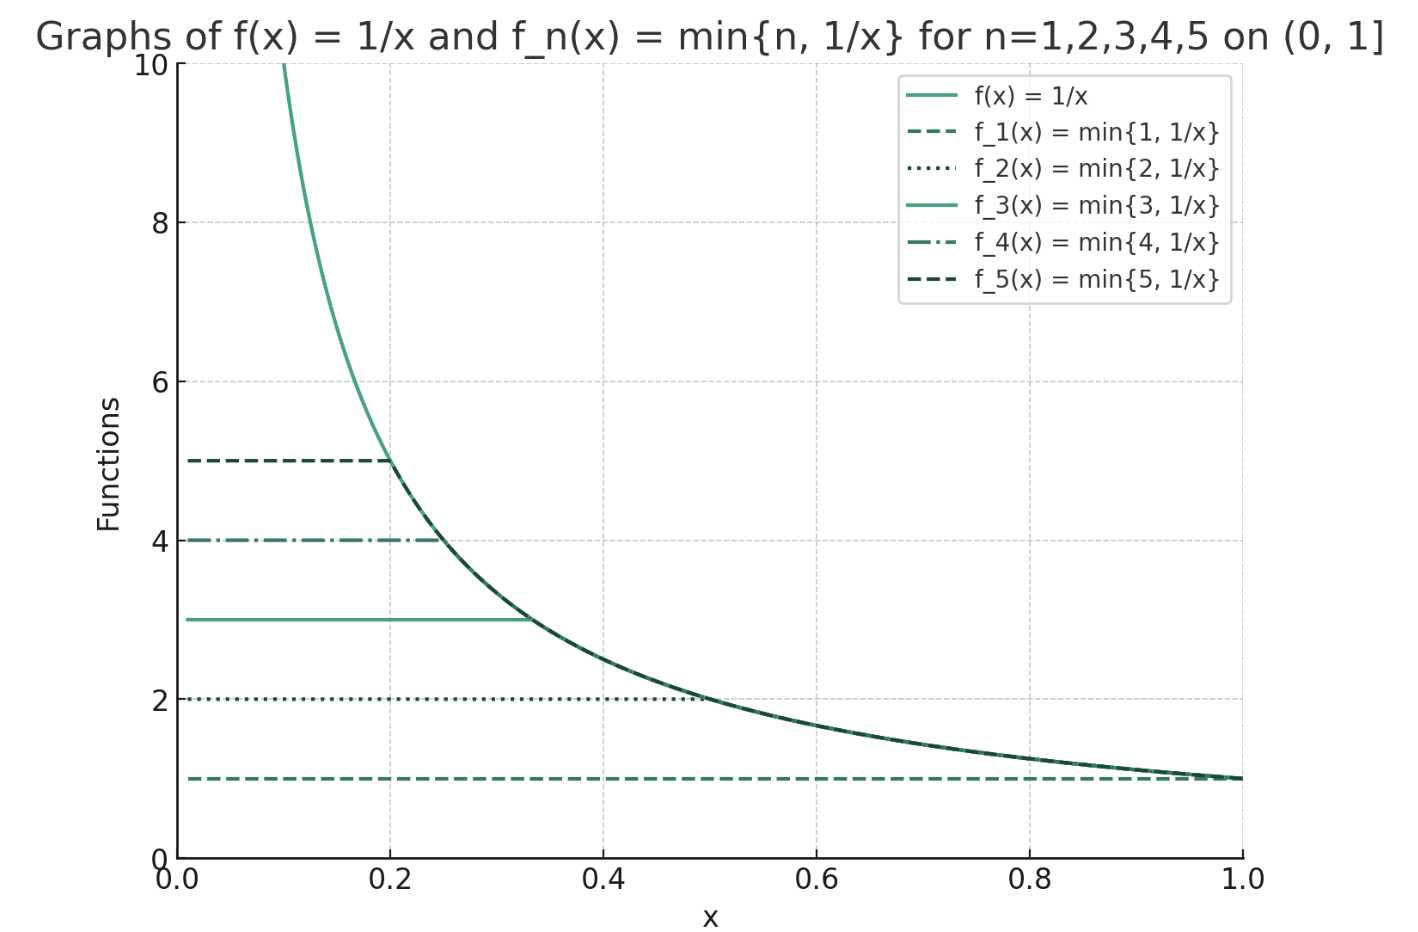
\includegraphics[height=9cm,width=15cm]{pwise converge1.png}
   \end{minipage}
\end{center}
\end{Example}
\begin{Example}{\textbf{(Unbounded functions pointwise converge to bounded function)}}{}
\begin{align*}
X=\R,f_n(x)=\frac{1}{n}x
\end{align*}
The limit function is $f(x)=0$
\begin{center}
   \begin{minipage}{0.9\linewidth}  
       \centering  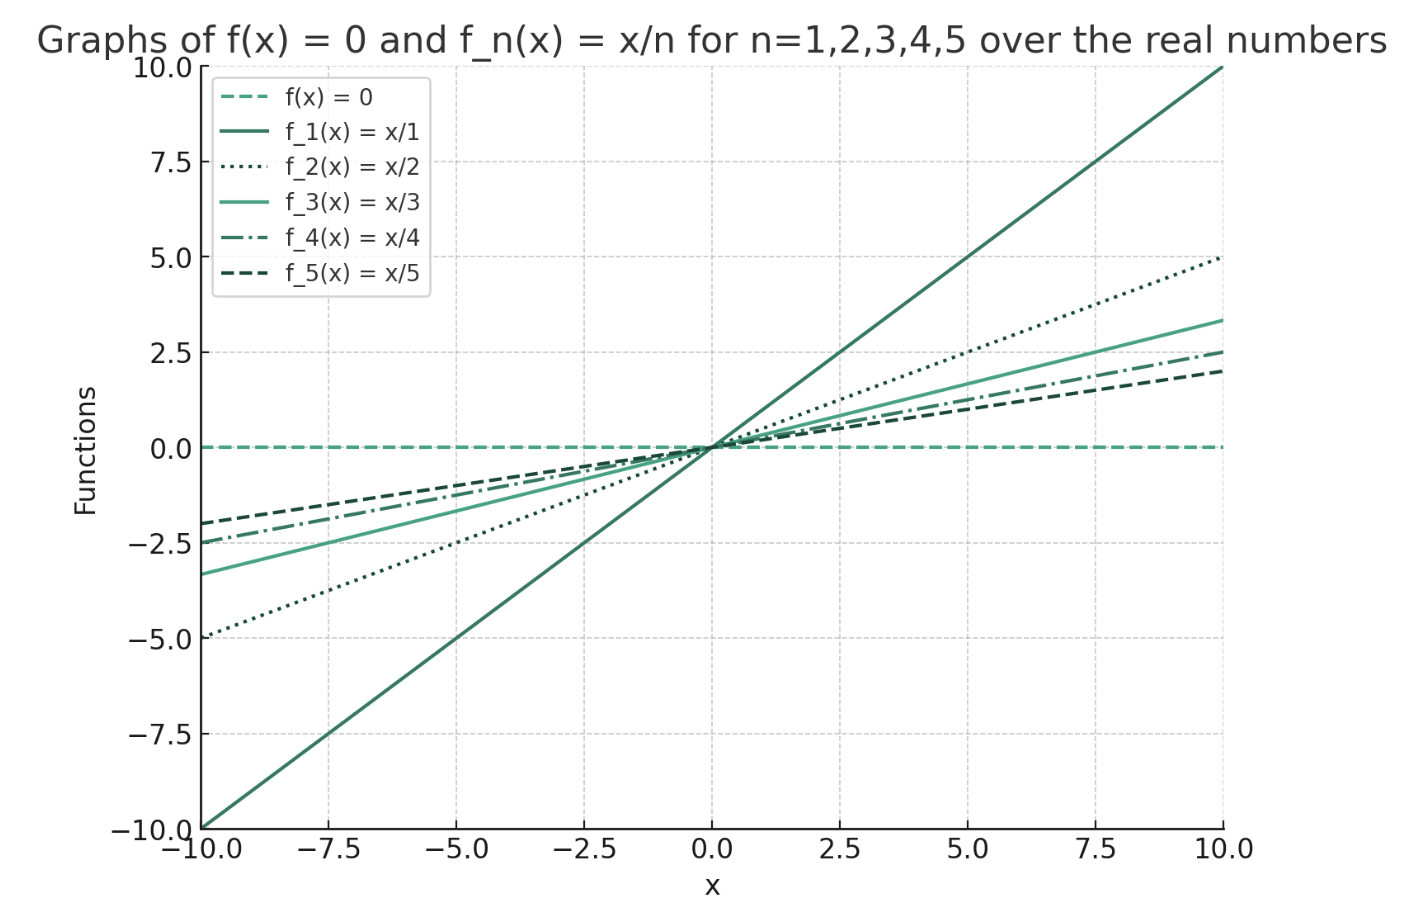
\includegraphics[height=7cm,width=15cm]{pwise converge2.png}
   \end{minipage}
\end{center}
\end{Example}
\end{mdframed} 
\begin{mdframed}
As pointed out earlier, if $f:X\rightarrow (Y,d)$ is bounded and $g:X\rightarrow (Y,d)$ is unbounded, then $d_{\infty}(f,g)=\infty$. This means that if $Y$ is unbounded, the uniform metric $d_{\infty}$ is extended on $X^Y$. For this, it is necessary to develop some basic fact concerning extended metric space.\\

Suppose $(X,d)$ is an extended metric space. If we define $\sim$ on $X$ by $x \sim y\iff  d(x,y)<\infty$, then $\sim $ is an equivalence relation. We say each equivalence class is a \textbf{galaxy} of $(X,d)$. Suppose $T$ is the collection of the galaxies of $(X,d)$. For each $\mathcal{T} \in T$, the space $(\mathcal{T},d)$ is just a metric space.\\

It is easy to see that the way we induce topology from metric space is still valid if the metric is extended. That is 
\begin{align*}
  \tau=\set{Z \in X: \forall z \in Z, \exists \epsilon ,B_\epsilon (z)\subseteq Z}
\end{align*}
is still a topology, even though $d$ is an extended metric on $X$.\\

We can verify that a set $Y$ in $X$ is open if and only if for all  $\mathcal{T} \in T$, the set $Y \cap \mathcal{T}$ is open, and the set $Y$ in $X$ is closed if and only if all convergent sequences $y_n$ in  $Y$ converge to points in $Y$. \\
\end{mdframed}
\begin{mdframed}
Now, suppose we are given an arbitrary set  $X$ and a complete metric space  $(\overline{Y},d)$, and on $X^{\overline{Y}}$, we define the uniform metric  $d_{\infty}$. We say a set $\mathcal{F}\subseteq X^{\overline{Y}}$ of functions is \textbf{closed under uniform convergence} if  for all uniform convergent sequence $f_n \subseteq \mathcal{F}$, the limit function $f$ is also in  $\mathcal{F}$. There are justified reasons for us to give the premise that $\overline{Y}$ is complete prior to the definition of the term \textbf{closed under uniform convergence}. One reason is that by \myref{Theorem}{Tsof}, if $Y$ is not complete, then the extended metric space  $(X^Y,d_{\infty})$ is also not complete, which implies the possibility a Cauchy sequence $f_n$ in  $X^Y$ converge to a function $f \in X^{\overline{Y}} \setminus X^Y$ where $\overline{Y}$ is the completion of  $Y$. For instance, if we let $Y=\R\setminus \set{1}$ where $X=\R$, and let $f_n(x)=\begin{cases}
  0& \text{ if  }x\neq 0\\
  1+\frac{1}{n}& \text{ if $x=0$ }
\end{cases}\in Y$, we see that the set $\mathcal{F}=\set{f_n:n\inn}$ is "closed under uniform convergence" in the context of $X^Y$, but when in fact $f_n$ uniformly converge to  $f(x)=\begin{cases}
  0& \text{ if  }x\neq 0\\
  1& \text{ if $x=0$ }
\end{cases}$ which is not in $\mathcal{F}$. This awkward usage of words can be solved if we define the term  \textbf{closed under uniform convergence} after the premise that $Y$ is complete.\\

Now, given a set of functions $\mathcal{F}\subseteq X^{\overline{Y}}$, one can verify that 
\begin{align*}
  \mathcal{F}\text{ is closed under uniform convergence }&\iff (\mathcal{F},d_{\infty})\text{ is complete }\\
&\iff \mathcal{F}\text{ is closed with respect to $(X^{\overline{Y}},d_{\infty})$ }
\end{align*}
Let $\mathcal{G}$ be a galaxy of $(X^{\overline{Y}},d_{\infty})$. With multiple ways, we can verify that $\mathcal{G}$ is closed with respect to $(X^{\overline{Y}},d_{\infty})$. Then, acknowledging the space of bounded functions $B(X,\overline{Y})$ is a galaxy of $X^{\overline{Y}}$, we see that $B(X,\overline{Y})$ is closed under uniform convergence. The statement that $B(X,\overline{Y})$ is closed under uniform convergence, although already "proved" before as we pointed out the limit of uniform convergent sequence of bounded functions must be bounded, is now in fact actually proved in the sense the term "closed under uniform convergence" is formally given a satisfying definition.
\end{mdframed}
\section{Arzelà–Ascoli Theorem}
\begin{mdframed}
In this section, we will give a complete proof of Arzelà–Ascoli Theorem for functions from arbitrary compact topological space to arbitrary metric space. Note that in Baby Rudin, Arzelà–Ascoli Theorem are given for functions from compact metric space to metric space. Because Arzelà–Ascoli Theorem are concerned with family of equicontinuos functions, it is crucial for us to give a definition to equicontinuity for functions from topological  space to metric space, for the sake of our generalization.\\

Let $X,Y$ be metric space. Let  $Z$ be topological space. Let  $\mathcal{F}_X$ be family of functions from $X$ to  $Y$, and let  $\mathcal{F}_Z$ be family of functions from $Z$ to  $Y$. We say  $\mathcal{F}_Z$ is \textbf{pointwise equicontinuous} if 
\begin{center}
   \begin{minipage}{0.9\linewidth}  
       \centering
       For all $\epsilon $ and for all $x$, there exists a neighborhood $U_x$ such that  $d_Y(f(x),f(y))<\epsilon $ for all $y \in U_x$   
   \end{minipage}
\end{center}
We say $\mathcal{F}_X$ is \textbf{equicontinuous} if 
\begin{center}
   \begin{minipage}{0.9\linewidth}  
       \centering
       For all $\epsilon $, there exists $\delta$ such that  $d_{Y}(f(x),f(y))<\epsilon $ for all $\delta$-close $x,y \in X$ and all  $f \in \mathcal{F}$. 
   \end{minipage}
\end{center}
It is easy to verify that if $\mathcal{F}_X$ is equicontinuous, then $\mathcal{F}_X$ is pointwise equicontinuous. The converse don't always hold true. Say, $\mathcal{F}=\set{n+x^2}_{n\inn}$, the set $\set{n+x^2}_{n\inn}$ is clearly pointwise equicontinuous on $\R$, and is not equicontinuous on $\R$, since no function $n+x^2$  is uniform continuous on $\R$. However, the same set $\mathcal{F}=\set{n+x^2}$ is equicontinous on compact domain $[a,b]$. This is a general result, as we shall prove below.
\end{mdframed}
\begin{theorem}
\textbf{(Pointwise Equicontinous is Uniform on Compact Domain)} Given two metric space $(X,d_X),(Y,d_Y)$, and a family $\mathcal{F}$ of functions from $X$ to  $Y$ such that 
 \begin{enumerate}[label=(\alph*)]
  \item $X$ is compact 
   \item $\mathcal{F}$ is pointwise equicontinuous
\end{enumerate}
Then 
\begin{align*}
\mathcal{F}\text{ is equicontinuous }
\end{align*}
\end{theorem}
\begin{proof}
Fix $\epsilon $. We wish to 
\begin{align*}
\vi{\text{ find $\delta$ such that $d_X(x,y)<\delta \implies d_Y(f(x),f(y))\leq \epsilon $ for all $f \in \mathcal{F}$ }}
\end{align*}
Because $\mathcal{F}$ is pointwise equicontinuous, we know for each $x \in X$, there exists $\delta_x$ such that 
\begin{align}
\label{PEe1}
\forall y\in B_{\delta_x}(x), d_Y\big(f(x),f(y) \big)<\frac{\epsilon}{2} \text{ for all $f\in \mathcal{F}$ }
\end{align}
It is clear that $\set{B_{\frac{\delta_x}{2}}(x):x \in X}$ form an open cover of $X$. Then because  $X$ is compact, we know  
 \begin{align*}
\text{ there exists a finite open sub-cover: }\set{B_{\frac{\delta_x}{2}}(x):x \in X_{\text{finite}}}
\end{align*}
We claim 
\begin{align*}
\vi{\delta=\min_{x \in X_{\text{finite}}}\frac{\delta_x}{2}\text{ works }}
\end{align*}
Fix $y,z \in X: d_X(y,z)<\delta$. We have to prove 
\begin{align*}
\vi{d_Y\big(f(y),f(z) \big)< \epsilon }
\end{align*}
We know $y$ must lie in some  $B_\frac{\delta_x}{2}(x)$ for some $x \in X_\text{finite}$. Because $d_X(y,z)<\frac{\delta_x}{2}$, we see that $z$ must lie in  $B_{\delta_x}(x)$. We now know $y,z$ are both in  $B_{\delta_x}(x)$. Then from \myref{(}{PEe1}), we can now deduce 
\begin{align*}
d_Y\big(f(y),f(z) \big)\leq d_Y\big(f(y),f(x) \big)+d_Y\big(f(x),f(z) \big)< \epsilon \vdone
\end{align*}
\end{proof}
\begin{mdframed}
The proof above should be a great example why in the discussion of metric space, instead of using sequential definition of compactness, which leads to the beautiful Bolzano-Weierstrass Theorem, some people prefer the open-cover definitions.\\

Now, we give proof for the Arzelà–Ascoli Theorem. 
\end{mdframed}
\begin{theorem}
\textbf{(Arzelà–Ascoli Theorem)} Given a compact topological space $(X,\tau)$, a metric space $(Y,d_Y)$, and a family $\mathcal{F}\subseteq C\big(X,Y \big)$ of continuous function  
 \begin{align*}
&\mathcal{F}\text{ is pointwise equicontinuous and $\set{f(x):f \in \mathcal{F}}$ has compact closure in $Y$ for all $x \in X$}\\
&\implies \mathcal{F}\text{ has a compact closure in $C(X,Y)$}
\end{align*}
\end{theorem}
\begin{proof}
Fix a sequence $f_n$ in $\mathcal{F}$. We wish to show
\begin{align*}
\vi{f_n\text{ has a sub-sequence $f_{n_k}$ uniformly converge to some }f:X\rightarrow Y}
\end{align*}
First, we prove 
\begin{align*}
\blue{\text{ there exists a countable set $P$ such that $P$ works like a dense set }}
\end{align*}
Because $\mathcal{F}$ is pointwise equicontinuous, we know for all $x \in X$ 
\begin{align*}
\exists U_{x,n}, \forall y \in U_{x,n},\forall f \in \mathcal{F}, d_Y\big(f(x),f(y) \big)<\frac{1}{n} \text{ for each fixed $n\inn$ }
\end{align*}
Now, because $X$ is compact, for each $n\inn$, there exists a finite subset $P_n\subseteq X$ such that $\bset{U_{x,n}:x \in P_n}$ is a cover of $X$. Let $P=\bigcup_{n\inn}P_n$. $\bdone$\\

Now, we wish to 
\begin{align*}
\olive{\text{ construct a sub-sequence $f_{n_k}$ pointwise converge on $P$ }}
\end{align*}

Express $P=\set{p_k}_{k\inn}$. By premise (pointwise image has compact closure), we know there exists a compact set that contain $\set{f_n(p_1)}_{n\inn}$, so by Bolzano-Weierstrass Theorem, there exists a sub-sequence 
\begin{align*}
\bset{f_{g_1(k)}(p_1)}_{k\inn}\text{ converge to some point in $Y$ }
\end{align*}
Now, again by premise and Bolzano-Weierstrass Theorem, there exists a sub-sequence 
\begin{align*}
\bset{f_{g_2\circ g_1(k)}(p_2)}_{k\inn}\text{ converge to some point in $Y$ }
\end{align*}
Repeatedly doing such, we have 
\begin{align*}
\begin{matrix} 
  f_{g_1(1)}(p_1) & f_{g_2\circ g_1 (1)}(p_2) & f_{g_3\circ g_2 \circ  g_1 (1)}(p_3) & \cdots \\
  f_{g_1(2)}(p_1) & f_{g_2\circ g_1 (2)}(p_2) & f_{g_3\circ g_2 \circ  g_1 (2)}(p_3) & \cdots \\
  f_{g_1(3)}(p_1) & f_{g_2\circ g_1 (3)}(p_2) & f_{g_3\circ g_2 \circ  g_1 (3)}(p_3) & \cdots \\
  \vdots &\vdots &\vdots & \ddots\\
  \downarrow & \downarrow &\downarrow &\\
  y_1 & y_2 & y_3 & \cdots 
\end{matrix}
\end{align*}
Now, let 
 \begin{align*}
n_k=g_k\circ \cdots \circ g_1(k)
\end{align*}
Then 
\begin{align*}
n_k\text{ is eventually a sub-sequence of $g_m\circ \cdots \circ g_1(k)$ for all $m$ }
\end{align*}
This then implies 
\begin{align*}
f_{n_k}(p_m)\to y_m\text{ for all $p_m \in P \odone$ }
\end{align*}
Next, we show 
\begin{align*}
\blue{\text{ To prove $f_{n_k}$ uniformly converge on $X$, it suffice to prove $f_{n_k}$ is uniformly Cauchy on $X$. }}
\end{align*}
By premise (pointwise image has compact closure), if $f_{n_k}$ is uniformly Cauchy, then we know $f_{n_k}$ pointwise converge to some $f$.\\

Fix $\epsilon $. We reduced the problem into 
\begin{align*}
\blue{\text{ finding  $N$ such that for all $k>N$, we have  $d_Y\big(f_{n_k}(x), f(x)\big)\leq \epsilon $ for all $x\in X$ }}
\end{align*}
Because $f_{n_k}$ is uniformly Cauchy, we know there exists $N$ such that for all $m,k>M$ $d_Y\big(f_{n_k}(x),f_{n_m}(x) \big)\leq \frac{\epsilon}{2}$ for all $x \in X$. We claim 
\begin{align*}
 \blue{\text{ such $N$ works }}
\end{align*}
Let $k>N$.  \As{$d_Y\big(f_{n_k}(x),f(x) \big)>\epsilon $}. We see that 
 \begin{align*}
   d_Y\big(f(x),f_{n_m}(x) \big)\geq d_Y\big(f(x),f_{n_k}(x)\big)-d_Y\big(f_{n_k}(x),f_{n_m}(x) \big)>\frac{\epsilon}{2}\text{ for all $m>N\tCaC \bdone$} 
\end{align*}
Lastly, we wish to prove 
\begin{align*}
\vi{f_{n_k}\text{ is uniformly Cauchy }}
\end{align*}
Fix $\epsilon $. We wish  
\begin{align*}
\vi{\text{ to find }N\text{ such that }\forall j,k >N,\forall x\in X, d_Y\big(f_{n_j}(x),f_{n_k}(x)\big)\leq \epsilon  }
\end{align*}
Fix $m > \frac{3}{\epsilon }$. Express $P_m=\set{p^m_1,\dots ,p^m_u}$. Because $f_{n_k}(p^m_t)$ converge for each $t \in \set{1,\dots ,u}$, we know 
\begin{align*}
\forall t , \exists N_t, d_Y\big(f_{n_j}(p_t^m),f_{n_k}(p_t^m) \big)<\frac{\epsilon}{3}\text{ for all $j,k>N_t$ }
\end{align*}
We claim 
\begin{align*}
\vi{N=\max_t N_t\text{ works }}
\end{align*}
Fix $j,k>N$ and $x \in X$. We have to show 
\begin{align*}
  \vi{d_Y\big(f_{n_j}(x),f_{n_k}(x) \big)\leq \epsilon}
\end{align*}
Because $\set{U_{p_t^m,m}}$ form an open cover of $X$, we know there exists  $t$ such that $x \in U_{p_t^m,m}$. We can now deduce 
\begin{align*}
d_Y\big(f_{n_j}(x),f_{n_k}(x) \big)\leq d_Y\big(f_{n_j}(x),f_{n_j}(p_t^m) \big)+d_Y\big(f_{n_j}(p_t^m),f_{n_k}(p_t^m) \big)+d_Y\big(f_{n_k}(p_t^m),f_{n_k}(x) \big)<\epsilon 
\end{align*}
$\vdone$\\

\end{proof}
\section{Banach Fixed Point Theorem}
\begin{mdframed}
This section give a complete statement and proof of Banach Fixed Point Theorem. The setting is 
\begin{enumerate}[label=(\alph*)]
  \item a metric space $\Big(X,d_X \Big)$ 
  \item a subset $E\subseteq X$
  \item another metric space $\Big(Y,d_Y \Big)$ 
  \item a function $f:E\rightarrow Y$ 
  \item another function $g:E\rightarrow X$
\end{enumerate}
We say $f$ is a \textbf{contraction} on $E$ if there exists $r\in [0,1)$ such that 
\begin{align*}
\hspace{3cm}d_Y(f(x),f(y))\leq rd_X(x,y)\hspace{1.5cm}(x,y \in E)
\end{align*}
or equivalently 
\begin{align*}
\sup_{x\neq y \in E} \frac{d_Y(f(x),f(y))}{d_X(x,y)}<1
\end{align*}
Note that the restriction of a contraction is again a contraction. We say $g$ admits a \textbf{fixed point} $x$ if we have 
\begin{align*}
g(x)=x
\end{align*}
\end{mdframed}
\begin{theorem}
\label{BFPT}
\textbf{(Banach Fixed Point Theorem)} If $g$ is a contraction that maps $E$ into $X$, then 
\begin{align*}
g\text{ admits at most one fixed point }
\end{align*}
Moreover, if $E$ is complete and $g(E)\subseteq E$, then 
\begin{align*}
\text{ the fixed point exists }
\end{align*}
And if we use the notation $g^n$ to denote $g\circ g^{n-1}$, then for all $x\in E$,  
\begin{align*}
  \text{ the fixed point can be written in the form }\lim_{n\to \infty}g^n(x)
\end{align*}
\end{theorem}
\begin{proof}
We first 
\begin{align*}
\vi{\text{ prove the uniqueness of the fixed point }}
\end{align*}
Suppose $x,y$ are both fixed by $g$.  We have
\begin{align*}
d(g(x),g(y))=d(x,y)
\end{align*}
Because  $g$ is a contraction mapping,  this implies $d(x,y)=0$. $\vdone$ \\

Suppose $E$ is complete and $g(E)\subseteq E$. We now 
\begin{align*}
\blue{\text{ prove the existence of the fixed point }}
\end{align*}
Fix $x \in E$. Because we have already prove the uniqueness of the fixed point, we only have to prove 
\begin{align*}
\blue{\lim_{n\to \infty}g^n(x)\text{ exists and }\lim_{n\to \infty}g^n(x)\text{ is a fixed point of $g$ }}
\end{align*}
Because $E$ is complete, to prove $\lim_{n\to \infty}g^n(x)$ exists, we only have to prove
\begin{align*}
\olive{\set{g^n(x)}_{n\inn}\text{ is Cauchy }}
\end{align*}
Observe 
\begin{align*}
  d(g^n(x),g^{n+k}(x))&\leq \sum_{i=0}^{k-1}d(g^{n+i}(x),g^{n+i+1}(x))\\
  &\leq d(x,g(x))\sum_{i=0}^{k-1}r^{n+i}\\
  &\leq \frac{r^n}{1-r}d(x,g(x))\to 0\text{ as $n\to \infty$ }\odone
\end{align*}
Note that contraction is Lipschitz thus continuous, and note that $\lim_{n\to \infty}g^n(x) \in E$. This allow us to carry the below limit process 
\begin{align*}
  g\big(\lim_{n\to \infty}g^n(x)\big)=\lim_{n\to \infty}g(g^n(x))=\lim_{n\to \infty}g^{n+1}(x)=\lim_{n\to \infty}g^n(x)\bdone
\end{align*}
\end{proof}
\begin{mdframed}
Banach Fixed Point Theorem is one of the most important Theorem in Mathematics. It will be used to prove 
\begin{enumerate}[label=(\alph*)]
  \item Inverse Function Theorem (\myref{Theorem}{IFT}) 
  \item Picard-Lindelof Theorem  
  \item Nash-Embedding Theorem
\end{enumerate}
\end{mdframed}
\chapter{Calculus}
\section{$\sigma$-algebra} 
\begin{mdframed}
In this section, we give the definition of $\sigma$-algebra, and the definition of the two important sub-structures, i.e. ring of sets and  $\sigma$-ring. We also prove some basic properties of these structures.
\end{mdframed}
\begin{definition}
\textbf{(Definition of Ring of Sets, $\sigma$-Ring and $\sigma$-Algebra)} Given a set $X$ and an non-empty set $R$ of subsets of $X$, suppose $A,B$ is arbitrary element of $R$. We say  $R$ is a  \textbf{ring of set} if 
\begin{enumerate}[label=(\alph*)]
  \item $A\cup B \in R$ (closed under finite union)
  \item $A\setminus B \in R$ (closed under relative complement)
\end{enumerate}
Moreover, we say $R$ is a  \textbf{$\sigma$-ring} if for all countable $\set{A_n} \subseteq R$, we have
\begin{align*}
\bigcup_{n} A_n \in R \text{ (closed under countable union) }
\end{align*}
Even more, we say $R$ is a  \textbf{$\sigma$-algebra} or \textbf{$\sigma$-field} if 
\begin{align*}
X \in R\text{ (universal set) }
\end{align*}
\end{definition}
\begin{mdframed}
Note that 
\begin{align*}
\varnothing = A \setminus  A
\end{align*}
This implies a ring of set $R$ must contain the empty set  $\varnothing$.
\begin{align*}
A\cap B= A\setminus (A\setminus B)
\end{align*}
This implies ring of sets $R$ is also closed under finite intersection. One may conjecture that we can give a different axioms to ring of set by changing finite union closure to finite intersection closure. This is false. See the following example. 
\end{mdframed}
\begin{Example}{\textbf{(Failure of Alternative Axioms)}}{}
\begin{align*}
X=\set{1,2,3}\text{ and }R=\set{\set{1,2},\set{2,3},\set{1},\set{2},\set{3},\varnothing}
\end{align*}
Check that $R$ is closed under finite intersection and relative complement. Observe that $\set{1,2}\cup  \set{2,3}\not\in R$. 
\end{Example}
\begin{mdframed}
Note that 
\begin{align*}
\bigcap_{n=1}^{\infty} A_n= A_1 \setminus \bigcup_{n=2}^{\infty} (A_1 \setminus A_n)
\end{align*}
This implies $\sigma$-ring is also closed under countable intersection. 
\end{mdframed}
\begin{Example}{\textbf{(Set of Elementary Sets is a  Ring of Sets that isn't a  $\sigma$-Ring)}}{}
\begin{align*}
&X=\R^n
\end{align*}
$R$ is the set of all subsets of $X$ that can be expressed as a finite union of \textbf{boxes}, sets of the form $\prod_{k=1}^n I_k$, in which $I_k\subseteq \R$ is a bounded interval. The elements of $R$ is called the  \textbf{elementary sets}. It is clear that $R$ is closed under finite union. Observe that given any two elementary sets $\bigcup_{k=1}^n A_k,\bigcup_{k=1}^m B_k$, we have 
\begin{align*}
\Big(\bigcup_{i=1}^n A_i \Big)\setminus \Big(\bigcup_{j=1}^m B_j \Big)=\bigcup_{i=1}^n \bigcap_{j=1}^m A_i \setminus  B_j
\end{align*}
Now, using the fact that $B_j^c$ is a union of (unbounded) boxes, $A_i \setminus  B_j= A_i \cap B_j^c$ and that intersection of boxes is again a box, we see $\bigcup_{i=1}^n A_i \setminus \bigcup_{j=1}^m B_j$ is an elementary set.\\

We have shown that $R$ is a ring of set. It is trivial to construct an counter-example when $X=\R$. 
\end{Example}
\begin{mdframed}
Note that given any $\sigma$-ring $R$ on $X$, one can always construct a  $\sigma$-algebra $\mathcal{A}$ by 
\begin{align*}
\mathcal{A}\triangleq \set{E \subseteq X: E\in R\text{ or }E^c \in R}
\end{align*}
Use the fact $R$ is closed under countable and De Morgan's Law, one can check that $\mathcal{A}$ is a $\sigma$-algebra.\\

Given a set $T$ of subsets of $X$, by the term \textbf{$\sigma$-algebra generated by} $T$ we mean the smallest $\sigma$-algebra $\sigma(T)$ containing $T$. Such  $\sigma(T)$ always exists, since the power set of  $X$ is a  $\sigma$-algebra containing $T$ and intersection of $\sigma$-algebra is again a $\sigma$-algebra.\\

Immediately, one can check that 
\begin{align*}
\mathcal{A}=\sigma (R)
\end{align*}
by showing every $\sigma$-algebra containing $R$ also contains  $\mathcal{A}$.
\end{mdframed}
\section{"top down" V.S. "buttom up" definition of Borel space; Borel hierarchy}
\begin{theorem}
\textbf{(Borel Hierarchy)}
\end{theorem}
\section{Property of measurable functions}
\begin{mdframed}
In this section, we give two equivalent general definition (\myref{Theorem}{EDm}) of measurable function and show
\begin{enumerate}[label=(\alph*)]
  \item Measurable $f:X\rightarrow \R\text{ or }\C$  is closed under addition and multiplication. (\myref{Theorem}{Btsa})
  \item The (superior) limit of a sequence of measurable ($\R\cup \set{\pm \infty} $ or $\C\cup \set{\infty}$)-valued functions on general $(X,\Sigma_X)$ is measurable. (\myref{Theorem}{Slm})
  \item Positive and negative part of a measurable $f:X\rightarrow [-\infty,\infty]$ are measurable. (\myref{Corollary}{PaN})
\end{enumerate}
\end{mdframed}
\begin{mdframed}
If we are given a function $f:(X,\Sigma_X)\rightarrow (Y,\Sigma_Y)$ such that for all $E\in \Sigma_Y$, we have $f^{-1}(E) \in \Sigma_X$, then we say $f$ is a  \textbf{measurable function}. Immediately, one can check that the composition of two measurable functions must be measurable. We now introduce an equivalent definition of measurable function, which makes checking if a function is measurable much easier.
\end{mdframed}
\begin{theorem}
\label{EDm}
\textbf{(Equivalent Definition of measurable function)} If a function $f:(X,\Sigma_X)\rightarrow (Y,\sigma (T))$ satisfy 
\begin{align*}
f^{-1}(E)\in \Sigma_X\text{ for all $E \in T$ }
\end{align*}
then 
\begin{align*}
f\text{ is measurable }
\end{align*}
\end{theorem}
\begin{proof}
Define 
\begin{align*}
\mathcal{A}\triangleq \set{E \subseteq Y: f^{-1}(E)\in \Sigma_X}
\end{align*}
Check that $\mathcal{A}$ is a $\sigma$-algebra on $Y$. By premise, $T \subseteq \mathcal{A}$. It then follows from definition that $\sigma (T)\subseteq \mathcal{A}$. This conclude that $f$ is  $(\Sigma_X, \sigma(T))$-measurable. 
\end{proof}
\begin{mdframed}
There are two important consequences of \myref{Theorem}{EDm}
\begin{enumerate}[label=(\alph*)]
  \item If $X,Y$ are both Borel, then a continuous function  $f:X\rightarrow Y$ must also be a measurable function. 
  \item If there exists $T$ such that  $\Sigma_Y=\sigma (T)$, then we only have to check that $f^{-1}(E)\in \Sigma_X$ for all $E \in T$ to show $f$ is measurable. In particular, if $Y=\R^n$, then  $T$ can be just the set of all open boxes.
\end{enumerate}
These two consequences give the following Lemma, which later prove \myref{Theorem}{Btsa}, Theorem that make checking if $\C\text{ or }\R$-valued function is measurable easier.
\end{mdframed}
\begin{lemma}
\label{CL}
\textbf{(Computational Lemma)} Given two measurable function $u,v:(X,\Sigma_X)\rightarrow \R$ and a continuous function $\Phi:\R^2 \rightarrow (Y,\tau_Y)$, define $h:(X,\Sigma_X)\rightarrow (Y,\mathcal{B}_Y)$ by
\begin{align*}
h(x)\triangleq \Phi(u(x),v(x))
\end{align*}
We can deduce
\begin{align*}
h:(X,\Sigma_X)\rightarrow (Y,\mathcal{B}_Y)\text{ is measurable }
\end{align*}
\end{lemma}
\begin{proof}
Define $f:X\rightarrow \R^2$ by $f(x)\triangleq (u,v)(x)$. Because $h=\Phi \circ f$, we can reduce the problem into proving
\begin{align*}
\vi{f\text{ is measurable }}
\end{align*}
Fix an open-rectangle $I_1\times I_2 \subseteq \R^2$. Because $\mathcal{B}_{\R^2}$ can be generated by the set of all open rectangles, we can reduce the problem into proving 
\begin{align*}
  \vi{f^{-1}(I_1\times I_2) \in \Sigma_X}
\end{align*}
Because $u,v$ are measurable, we know
\begin{align*}
f^{-1}(I_1\times I_2)=u^{-1}(I_1)\cap v^{-1}(I_2) \in \Sigma_X \vdone
\end{align*}
\end{proof}
\begin{theorem}
\label{Btsa}
\textbf{(Basic tools to show a real/complex-valued function is measurable)} Given a measurable set $X$, and two real-valued function $u,v:X\rightarrow \R$
\begin{enumerate}[label=(\alph*)]
  \item  $u+iv:X\rightarrow \C$ is measurable if and only if $u,v$ are measurable.
  \item If  $f,g:X\rightarrow \R\text{ or }\C$ are measurable, so are $f+g,fg\text{ and }\abso{f}$.
  \item If $f:X\rightarrow \R\text{ or }\C$ is measurable and $g:X\rightarrow \R\text{ or }\C$ isn't, then $f+g$ is not measurable.
  \item If $f:X\rightarrow \C$ is measurable, then there exists $\alpha :X\rightarrow \C$ such that $\abso{\alpha }=1$ and $f=\alpha \abso{f}$
\end{enumerate}
\end{theorem}
\begin{proof}
(a) follows from \myref{Lemma}{CL} and noting $u=\text{Re}(u+iv),v=\text{Im}(u+iv)$, since Re,Im $:\C\rightarrow \R$ are continuous.\\

(b) follows from the fact $\R,\C$ are topological field and \myref{Lemma}{CL}. \\

It is clear that the set of all function from  $X$ to $\R\text{ or }\C$ form a group under addition. (b) shows that the set of measurable functions from a subgroup, thus giving (c).\\

It remains to prove (d). Define 
\begin{align*}
E\triangleq \set{x \in X: f(x)=0}\text{ and }\phi(z)\triangleq  \frac{z}{\abso{z}}
\end{align*}
We claim 
\begin{align*}
  \vi{\alpha \triangleq \phi\circ (f+\textbf{1}_E)\text{ suffices }}
\end{align*}
Because $f$ is measurable, we know $E$ is measurable. This implies that $\textbf{1}_E:X\rightarrow \C$ is measurable. It follows that $f+\textbf{1}_E$ is $(X,\mathcal{B}_\C)$-measurable. Note that $f+\textbf{1}_E$ is never $0$ on $X$.\\


Now by \myref{Theorem}{}, we see $f+\textbf{1}_E$ is $(X,\mathcal{B}_{\C^*})$-measurable. It then follows from the fact  $\phi:\C^*\rightarrow \C$ is continuous that $\alpha $ is $(X,\mathcal{B}_\C)$ measurable.\\

Observe that $\alpha$ maps $E$ into $\set{1}$, and when $x\not\in E$, we have $\alpha (x)= \frac{f(x)}{\abso{f(x)}}$. $\vdone$
\end{proof}
\begin{mdframed}
Note that \myref{Theorem}{Btsa} does not consider function whose range include $\infty$. This will be later addressed using approximation of simple functions.
\end{mdframed}
\begin{theorem}
\label{Slm}
\textbf{(Superior limit of measurable $f_n:X\rightarrow [-\infty,\infty]$ is measurable)} Given a sequence $f_n:X\rightarrow [-\infty, \infty]$ of measurable functions
\begin{align*}
g\triangleq \sup f_n \text{ and }f\triangleq \limsup_{n\to\infty} f_n\text{ are both measurable }
\end{align*}
\end{theorem}
\begin{proof}
It is straightforward to check 
\begin{align*}
  g^{-1}(\alpha ,\infty] = \bigcup_n f_n^{-1} (\alpha ,\infty]
\end{align*}
It is straightforward to check
\begin{align*}
  \mathcal{B}_{[-\infty,\infty]}=\sigma \Big( \set{(\alpha ,\infty] \subseteq [-\infty,\infty]: \alpha \inr} \Big)
\end{align*}
These two facts and \myref{Theorem}{EDm} shows $g$ is measurable. The same arguments shows that $\inf g_k$ is measurable if $g_k$  are all measurable.\\

It is straight forward to check 
\begin{align*}
f= \inf_{n\geq 1} \sup_{k\geq n} f_k
\end{align*}
It then follows $f$ is measurable.
\end{proof}
\begin{corollary}
\label{Plm}
\textbf{(Pointwise limit of measurable $f_n:X\rightarrow [-\infty,\infty]$ is measurable)} If the sequence $f_n:X\rightarrow [-\infty,\infty]$ pointwise converge to $f:X\rightarrow [-\infty,\infty]$,  then $f$ is measurable. 
\end{corollary}
\begin{corollary}
\label{PaN}
\textbf{(Positive and Negative parts of a measurable function are measurable)} If we are given measurable $f:X\rightarrow [-\infty,\infty]$, and we define the \textbf{positive and negative part} $f^+,f^-:X\rightarrow [0,\infty]$ \textbf{of} $f$ by 
\begin{align*}
f^+\triangleq \max \set{f,0}\text{ and }f^- \triangleq -\min \set{f,0}
\end{align*}
Then 
\begin{align*}
f^+\text{ and }f^-\text{ are measurable }
\end{align*}
\end{corollary}
\begin{proof}
Define  
\begin{align*}
h_n\triangleq \begin{cases}
  f& \text{ if $n$ is odd }\\
  0& \text{ if $n$ is even }
\end{cases}
\end{align*}
then we have 
\begin{align*}
\limsup_{n\to\infty} h_n=f^+\text{ and }\liminf_{n\to\infty} h_n=-f^-
\end{align*}
Now, because $0$ is a measurable function, by \myref{Theorem}{Slm}, $f^+$ is measurable. Moreover, because $-1$ is a measurable function, by  \myref{Theorem}{Btsa}, $f^-$ is measurable.
\end{proof}
\section{Carathéodory's extension theorem}
\begin{definition}
\textbf{(Definition of pre-measure)} Given a $R$ ring of subsets of  $X$, we say  $\mu:R\rightarrow [0,\infty]$ is a \textbf{pre-measure} of $(X,R)$ if 
\begin{enumerate}[label=(\alph*)]
  \item $\mu(\varnothing)=0$ 
  \item $\mu\big(\bigcup E_n\big)=\sum \mu (E_n)$ for each countable disjoint $\set{E_n}$ such that $\bigcup E_n \in R$. (countably additive, or $\sigma$-additive)
\end{enumerate}
\end{definition}
\begin{mdframed}
It is straightforward to check 
\begin{enumerate}[label=(\alph*)]
  \item $\mu (A_1 \cup  \cdots \cup  A_n)= \mu (A_1) + \cdots + \mu (A_n)$ if each $A_i$ are disjoint.
  \item $A \subseteq B \implies \mu (A) \leq \mu (B)$
\end{enumerate}
\end{mdframed}
\begin{theorem}
\label{Bppm}
\textbf{(Basic property of pre-measure)} Given an increasing sequence of measurable set $A_n$ 
 \begin{align*}
\mu (A_n)\nearrow \mu (A)
\end{align*}
where $A=\bigcup A_n$. If $A_n$ is decreasing, then 
\begin{align*}
\mu (A_n)\searrow \mu (A)
\end{align*}
where $A=\bigcap A_n$.
\end{theorem}
\begin{proof}
If $A_n$ is increasing, fix $B_n\triangleq A_n\setminus A_{n-1}$ for each $n\geq 2$ and $B_1=A_1$. The proof then follows from checking 
\begin{align*}
\mu (A_n)= \sum_{k=1}^n \mu (B_k)\text{ and }\mu(A)=\sum_{k=1}^{\infty} \mu (B_k)
\end{align*}
The proof for another statement is similar.
\end{proof}
\begin{mdframed}
Using the same trick $B_n\triangleq A_n \setminus (A_{n-1}\cup  \cdots \cup A_1)$, we have 
\begin{align*}
\mu (\bigcup_{n\inn} A_n) \leq \sum_{n\inn} \mu (A_n)\text{ for arbitrary $A_n$ }
\end{align*}
\end{mdframed}
\begin{definition}
\textbf{(Definition of outer measure)} Given a set $X$, by an  \textbf{outer measure}, we mean a function $\mu^*:2^X\rightarrow [0,\infty]$ such that 
\begin{enumerate}[label=(\alph*)]
  \item $ \mu^* (\varnothing)=0$
  \item Given arbitrary subset $A,B_1,B_2,\dots$ such  that  $A\subseteq \bigcup_{n} B_n$, we have $ \mu^* (A)\leq  \sum_n \mu^* (B_n)$ (countably subadditive)
\end{enumerate}
\end{definition}
\begin{mdframed}
Equivalently, one can replace countably sub-additive with 
\begin{align*}
A \subseteq B \implies \mu^*(A) \leq \mu^* (B)\text{ and } \mu^* \Big(\bigcup_n B_n \Big)\leq \sum_n \mu^*(B_n)
\end{align*}
\end{mdframed}
\begin{theorem}
\textbf{(Pre-measure induces outer measure)} Given a pre-measure $\mu$ on some ring $R$ of subsets of $X$, if we define $\mu^*:2^X\rightarrow [0,\infty]$ by
\begin{align*}
\mu^*(T)\triangleq \inf \bset{\sum_n \mu (S_n):T \subseteq \bigcup _n S_n\text{ and }S_1,S_2,\dots \in R}\text{ where $\inf \varnothing= \infty$ }
\end{align*}
Then 
\begin{align*}
\mu^*\text{ is an outer measure }
\end{align*}
\end{theorem}
\begin{proof}
  It is clear $\mu^*(\varnothing)=0\text{ and }A\subseteq B \implies \mu^*(A)\leq \mu^*(B)$. It remains to prove for arbitrary $B_n$ we have 
\begin{align*}
  \vi{\mu^* \Big(\bigcup_n B_n \Big)  \leq \sum_n \mu^* (B_n)}
\end{align*}
If  $\sum_n \mu^*(B_n)=\infty$, the proof is trivial. We from now suppose $\sum_n \mu^*(B_n)< \infty$.\\

Fix $\epsilon $. We prove 
\begin{align*}
  \vi{\mu^*\Big(\bigcup _n B_n \Big)\leq \sum_n \mu^* (B_n)+\epsilon }
\end{align*}
Because $\mu^*(B_n)<\infty$ for each $n\inn$, we know for each $n\inn$ there exists an countable cover of $B_n$ consisting elements $S_{n,k}$ of  $R$ such that 
\begin{align*}
\sum_k \mu (S_{n,k}) \leq \mu^*(B_n)+\epsilon (2^{-n}) 
\end{align*}
It is clear that  $\set{S_{n,k}:n,k \inn}$ is a countable cover of $\bigcup_n B_n$, we now see 
\begin{align*}
  \mu^*\Big(\bigcup_n B_n \Big)&\leq \sum_n \sum_k \mu(S_{n,k})\\
&\leq \sum_n \mu^*(B_n)+ \epsilon (2^{-n})= \sum_n \mu^*(B_n)+ \epsilon \vdone
\end{align*}
\end{proof}
\begin{mdframed}
Note that 
\begin{align*}
\mu(A)=\mu^*(A)\text{ if $A\in R$ }
\end{align*}
\end{mdframed}
\begin{definition}
\textbf{(Definition of measure)} 
\end{definition}
\begin{theorem}
\textbf{(Outer measure induce measure)} We say a set $A\in 2^X$ is measurable if 
\begin{align*}
\mu^*(A)=\mu^* (A \cap  E)+ \mu^* (A \setminus E)\text{ for all $E \in 2^X$ }
\end{align*}
\end{theorem}
\begin{proof}

\end{proof}
\begin{theorem}
\textbf{(Measure induce complete measure)} 
\end{theorem}
\section{Lebesgue measure}
\begin{mdframed}
In this section, we develop the definition of Lebesgue measure.
\end{mdframed}
\section{Abstract integration} 
\begin{mdframed}
We say a function is a \textbf{simple function} if its range is of finite cardinality. Simple function is the cornerstone of the development of Lebesgue Integral Theory, as we shall see.\\

Suppose $s$ is a simple function defined on some measurable $E\subseteq (X,\Sigma_X)$ with range $\set{c_1,\cdots ,c_n}\subseteq [0,\infty]$. Define 
\begin{align*}
E_j\triangleq \set{x \in X: s(x)=c_j}
\end{align*}
It is clear that $\set{E_j}$ is a finite disjoint decomposition of $E$, and $s$ is measurable if and only if all $E_j$ are measurable.\\

We can write
\begin{align*}
s= \sum_{j=1}^n c_i \textbf{1}_{E_j}
\end{align*}
Then if $s$ is measurable, we can define
\begin{align*}
\int_E s d\mu \triangleq \sum_{j=1}^n c_j \mu (E_j)
\end{align*}
and if $s$ is defined on some larger domain while $s|_E$ is measurable, we can define 
\begin{align*}
\int_E s d\mu \triangleq \sum_{j=1}^n c_j\mu (E_j\cap E)
\end{align*}
Note that if $s$ is defined on some measurable $F$ containing  $E$ and  $s$ is measurable on $F$, then $s$ is surely measurable on $E$. It is straightforward to verify our definition so far is consistent.
\end{mdframed}


\begin{mdframed}
We now expand our definitions to the class of all measurable functions range in $[0,\infty]$.\\

Given a function $f$ range in $[0,\infty]$ and measurable on $E$, we define 
\begin{align*}
\int_E fd\mu \triangleq \sup_{s\leq f\text{ on }E} \int_E s d\mu
\end{align*}
If $f$ is defined on some large measurable domain $F$, we see that 
 \begin{align*}
\int_Efd\mu= \int_F f\textbf{1}_Ed\mu
\end{align*}
It is at this point one should verify our definition is so far consistent. That is, for each simple $s$, we have 
\begin{align*}
\int_Esd\mu=\sup_{s'\leq s\text{ on }E}\int_Es'd\mu
\end{align*}
The trick is to decompose each $E_j'$ into $\bigcup E_j'\cap E_i$. 
\end{mdframed}

\begin{mdframed}
We now expand our definitions to the class of all measurable functions range in $[-\infty,\infty]$, but before such, we have to first introduce the idea of \textbf{Lebesgue integrable}. For either $s$ or  $f$, range in either $[0,\infty)$ or $[0,\infty]$, it is always possible that $\int_E s\text{ or }fd\mu=\infty$.\\ 

If we have $\int_Efd\mu=\infty$, we say $f$ is \textbf{not Lebesgue integrable}, and if $\int_Efd\mu<\infty$, we say $f$ is \textbf{Lebesgue integrable on }$E$. Because $\R$ is complete in order, we know $f$ is either Lebesgue integrable or not Lebesgue integrable on $E$.\\

Given a function range in $[-\infty,\infty]$ and measurable on $E$, if both $f^+,f^-$ are Lebesgue integrable on $E$, we say  $f$ is Lebesgue integrable on $E$, and write 
\begin{align*}
\int_E fd\mu= \int_E f^+d\mu- \int_E f^-d\mu
\end{align*}
If either  $f^+$ or  $f^-$ are not Lebesgue integrable on $E$, we say $f$ is not Lebesgue integrable on $E$.\\

Notice that 
\begin{align*}
f\text{ is Lebesgue integrable on }E\iff \int_E \abso{f}d\mu<\infty
\end{align*}
It is clear that our definition is again so far consistent.
\end{mdframed}
\begin{mdframed}
We now 
\end{mdframed}

\section{Basic property of abstract integration}
\begin{mdframed}
This section prove some basic properties of Lebesgue integral over general measure space $(X,\Sigma_X,\mu)$. From now when we use the notation $X$, it shall be understood $X$ is equipped with an $\sigma$-algebra $\Sigma_X$ and a measure $\mu$. We will prove 
\begin{enumerate}[label=(\alph*)]
  \item Lebesgue Monotone Convergence Theorem (\myref{Theorem}{LMCT})
  \item Fatou's Lemma (\myref{Theorem}{Fatou})
  \item Reverse Fatou's Lemma (\myref{Theorem}{RFL}) 
  \item Dominated Convergence Theorem (\myref{Theorem}{LDCT})
\end{enumerate}
\end{mdframed}
\begin{theorem}
\label{LMCT}
\textbf{(Lebesgue Monotone Convergence Theorem)} Given a sequence of measurable $f_n:X\rightarrow [0,\infty]$ such that $\set{f_n(x)}_{n\inn}$ is an increasing sequence for each $x\in X$, then 
\begin{align*}
\int_X fd\mu = \lim_{n\to \infty}\int_X f_nd\mu
\end{align*}
\end{theorem}
\begin{proof}
$f$ is measurable by \myref{Corollary}{Plm}. Because  $f_n \nearrow f$ on $X$, we know 
\begin{align*}
 \lim_{n\to \infty}\int_X f_nd\mu = \sup_n \int_X f_nd\mu \leq \int_X fd\mu 
\end{align*}
It remains to prove 
\begin{align*}
\vi{\int_X fd\mu \leq \lim_{n\to \infty}\int_X f_nd\mu}
\end{align*}
Fix simple $0\leq s\leq f$ on $X$. We reduce the problem into proving 
\begin{align*}
  \vi{\int_X sd\mu \leq \lim_{n\to \infty}\int_X f_nd\mu}
\end{align*}
Fix $c \in (0,1)$. We reduce the problem into proving 
\begin{align*}
  \vi{c\int_X sd\mu \leq \lim_{n\to \infty}\int_X f_nd\mu}
\end{align*}
Define 
\begin{align*}
E_n \triangleq \set{x\in X: f_n(x)\geq cs(x)}
\end{align*}
$E_n$ are measurable because $f_n-cs$ are measurable. Now because $f_n$ are non-negative on  $X$, we have 
\begin{align*}
\int_X f_n d\mu \geq \int_{E_n}f_n d\mu \geq c \int_{E_n} sd\mu
\end{align*}
Taking limit, we see
\begin{align*}
\lim_{n\to \infty} \int_X f_n d\mu \geq \lim_{n\to \infty} c \int_{E_n}sd\mu 
\end{align*}
It is straightforward to check $E_n$ is increasing and $\bigcup E_n =X$. Then if we decompose $s=\sum_{j} c_j \textbf{1}_{F_j}$, by \myref{Theorem}{Bppm}, we can take limit 
\begin{align*}
\lim_{n\to \infty}\mu (F_j\cap E_n)=\mu (F_j)
\end{align*}
It then follows that 
\begin{align*}
\lim_{n\to \infty}\int_X f_nd\mu \geq \lim_{n\to \infty}c \int_{E_n}sd\mu= c\int_X sd\mu \vdone
\end{align*}
\end{proof}
\begin{mdframed}
It is worth pointing out in our proof for Lebesgue Monotone Convergence Theorem, instead of proving $\int_X sd\mu \leq \lim_{n\to \infty}\int_X f_nd\mu$, we proved $c\int_X sd\mu \leq \lim_{n\to \infty}\int_X f_nd\mu$. Multiplying $\int_X sd\mu$ with $c\in (0,1)$ is not just a random limit technique. Our action play a much more profound role. Consider the Example.
\end{mdframed}
\begin{Example}{\textbf{(Why we take $c\int_X sd\mu$ ?)}}{}
\begin{align*}
X=[0,1]\text{ and }f_n=1-\frac{1}{n}
\end{align*}
We can take $s=f$, and see $E_n=\varnothing$ for all $n$, which renders our proceeding proof invalid. 
\end{Example}
\begin{corollary}
\textbf{(Monotone Convergence Theorem for general functions)} Given a sequence of measurable $f_n:X\rightarrow [0,\infty]$ such that
\begin{enumerate}[label=(\alph*)]
  \item $\set{f_n(x)}_{n\inn}$ is an increasing sequence on $N^c$
  \item $f:X\rightarrow [0,\infty]$ is the limit of $f_n$ on $N^c$ 
  \item $\mu (N)=0$
  \item $\mu$ is complete
\end{enumerate}
We have 
\begin{align*}
\int_X fd\mu = \lim_{n\to \infty}\int_X f_nd\mu
\end{align*}
\end{corollary}
\begin{proof}
Let
\begin{align*}
g(x)\triangleq \begin{cases}
  f(x)& \text{ if $x \in N^c$ }\\
  0& \text{ if $x\in N$ }
\end{cases}
\end{align*}
Note that 



\begin{align*}
\int_X fd\mu = \int_{N^c}fd\mu = \lim_{n\to \infty}\int_{N^c} fd\mu = \lim_{n\to \infty} \int_X fd\mu
\end{align*}
\end{proof}
\begin{theorem}
\label{Fatou}
\textbf{(Fatou's Lemma)} Given measurable $f_n:X\rightarrow [0,\infty]$ 
\begin{align*}
\int_X \liminf_{n\to\infty} f_nd\mu \leq \liminf_{n\to\infty} \int_X f_n d\mu
\end{align*}
\end{theorem}
\begin{proof}
Since $\inf_{k\geq n}f_k\leq f_n$ for each $n,x$, we see 
 \begin{align*}
\int_X \inf_{k\geq n}f_k d\mu \leq \int_X f_nd\mu\text{ for all $n$ }
\end{align*}
Because $\inf_{k\geq n}f_k\nearrow  \liminf_{m\to\infty} f_m$ as $n\to \infty$, by (\myref{Theorem}{LMCT}: Lebesgue Monotone Convergence Theorem), we can take limit 
\begin{align*}
\int_X \liminf_{n\to\infty} f_n d\mu = \lim_{n\to \infty}\int_X \inf_{k\geq n}f_k d\mu\leq \liminf_{n\to\infty} \int_X f_nd\mu
\end{align*}
\end{proof}
\begin{Example}{\textbf{(Fatou's Lemma strict inequality)}}{}
\begin{align*}
f_{2k}(x)=\begin{cases}
 0& \text{ if $x\in [0,\frac{1}{2}]$ } \\
 1& \text{ if $x\in (\frac{1}{2},1]$ }
\end{cases}\text{ and }f_{2k+1}(x)=\begin{cases}
  1& \text{ if $x\in [0,\frac{1}{2})$ }\\
  0& \text{ if $x\in [\frac{1}{2},1]$ }
\end{cases}
\end{align*}
\end{Example}
\begin{mdframed}
  From now, we use $L^1(\mu)$ to denote the set of all function defined and $\mu$-Lebesgue-integrable on $X$, and we say a sequence of function  $f_n:X\rightarrow [0,\infty]$ is  \textbf{dominated} by $g$, if $g$ is a $[0,\infty]$-valued function defined on $X$ such that 
\begin{align*}
\sup_n \abso{f_n(x)} \leq g(x)\text{ for all $x\in X$ }
\end{align*}
\end{mdframed}
\begin{theorem}
\label{RFL}
\textbf{(Reverse Fatou's Lemma)} Given measurable $f_n:X\rightarrow [0,\infty]$ dominated by some $g \in L^1(\mu)$ 
\begin{align*}
\limsup_{n\to\infty} \int_X f_nd\mu \leq \int_X \limsup_{n\to\infty} f_nd\mu
\end{align*}
\end{theorem}
\begin{proof}
By (\myref{Theorem}{Fatou}: Fatou Lemma)
\begin{align*}
\int_X \liminf_{n\to\infty} (g-f_n) d\mu \leq \liminf_{n\to\infty} \int_X (g-f_n)d\mu 
\end{align*}
Multiplying both side with $-1$, we have 
\begin{align*}
\limsup_{n\to\infty} \int_X (f_n-g)d\mu \leq \int_X \limsup_{n\to\infty} (f_n-g)d\mu
\end{align*}
Then adding both side the constant $\int_X gd\mu$, we reach to the conclusion.
\end{proof}
\begin{mdframed}
Note that in our proof above, when we "pull" the negative sign out from $\liminf_{n\to\infty} $, it changed to $\limsup_{n\to\infty} $. This is a standard technique, which can be justified using the sub-sequence definition of limit superior.
\end{mdframed}
\begin{theorem}
\label{LDCT}
\textbf{(Dominate Convergence Theorem)} Given a sequence $f_n:X\rightarrow \C\cup \set{\infty}$ of measurable function such that 
\begin{align*}
f\triangleq \lim_{n\to \infty}f_n\text{ exists on $X$ }
\end{align*}
If there exists $g \in L^1(\mu)$ dominating $f_n$, then 
\begin{align*}
\lim_{n \to \infty} \int_X \abso{f_n-f}d\mu=0\text{ and }\int_X fd\mu = \lim_{n\to \infty} \int_X f_n d\mu\text{ exists in $\C\cup  \set{\infty}$ }
\end{align*}
\end{theorem}
\begin{proof}
Because $f$ is measurable by \myref{Corollary}{Plm} and  $\abso{f}\leq g$ on $X$, $f \in L^1(\mu)$.\\

We first prove 
\begin{align*}
  \vi{\lim_{n\to \infty}\int_X \abso{f_n-f}d\mu=0}
\end{align*}
We relax the problem into proving 
\begin{align*}
  \vi{\limsup_{n\to\infty} \int_X \abso{f_n-f}d\mu=0}
\end{align*}
Note that $\abso{f_n-f}\leq 2g$. We can now apply (\myref{Theorem}{Fatou}: Fatou lemma) to $2g- \abso{f_n-f}$ and see 
\begin{align*}
\int_X 2gd\mu&=   \int_X \lim_{n\to \infty}(2g- \abso{f_n-f})d\mu \\
&\leq \liminf_{n\to\infty} \int_X (2g-\abso{f_n-f})d\mu\\
&= \int_X 2gd\mu + \liminf_{n\to\infty} \Big(- \int_X \abso{f_n-f}d\mu \Big)\\
&=\int_X 2gd\mu - \limsup_{n\to\infty} \int_X \abso{f_n-f}d\mu
\end{align*}
Then because $g \in L^1(\mu)$, we can subtract it and obtain 
\begin{align*}
\limsup_{n\to\infty}\int_X  \abso{f_n-f}d\mu=0 \vdone
\end{align*}
It then follows that 
\begin{align*}
  \limsup_{n\to\infty} \abso{\int_X (f_n-f)d\mu} \leq \limsup_{n\to\infty} \int_X \abso{f_n-f}d\mu =0
\end{align*}
which implies 
\begin{align*}
\lim_{n\to \infty} \int_X (f_n-f)d\mu =0
\end{align*}
and because $f\in L^1(\mu)$, we have
\begin{align*}
\lim_{n\to \infty}\int_X f_nd\mu = \int_X fd\mu
\end{align*}
\end{proof}
\begin{Example}{\textbf{(Counterexample for Dominate Convergence Theorem)}}{}
\begin{align*}
f_n(x)=\begin{cases}
  \frac{1}{n}& \text{ if $\abso{x}<n$ }\\
  0& \text{ if $\abso{x}\geq n$ }
\end{cases}
\end{align*}
\end{Example}
\section{Riesz–Markov–Kakutani representation theorem}
\section{bounded variation}
\begin{mdframed}
This section prove some key properties of functions of bounded variations. These properties are worthy of discuss, as they make the set $BV\big([a,b] \big)$ of function of bounded variation on $[a,b]$ a natural candidate for the class of Riemann-Stieltjes integrator. The key properties include 
\begin{enumerate}[label=(\alph*)]
  \item Functions of bounded variation must be continuous almost everywhere. (\myref{Corollary}{Fmo})
  \item Functions of bounded variation can be expressed as difference of two increasing functions. (\myref{Theorem}{Fob}) 
  \item Functions of bounded variation can only have jump discontinuity. (\myref{Corollary}{Fobj})
\end{enumerate}
\end{mdframed}
\begin{definition}
\textbf{(Definition of variation and function of bounded variation)} Given a compact interval $[a,b]$, by a \textbf{partition} $P$ of $[a,b]$, we mean a finite set $\set{a=x_0<x_1 < \cdots < x_{n-1} < x_n =b}$ contain by $[a,b]$ and containing $a,b$. If  $f$ is a complex-valued function defined on $[a,b]$, we say the \textbf{total variation} $V_f(a,b)$ of $f$ on  $[a,b]$ is 
\begin{align*}
\sup_P \sum_{k=1}^n \abso{f(x_k)-f(x_{k-1})}
\end{align*}
We say $f$ is of \textbf{bounded variation} on $[a,b]$ if $V_f(a,b)<\infty$, and we denote the set of real-valued function from $[a,b]$ of bounded variation on $[a,b]$ by $BV\big([a,b] \big)$. 
\end{definition}
\begin{mdframed}
It is straightforward to check 
\begin{enumerate}[label=(\alph*)]
  \item  $f \in BV\big([a,b] \big)$ must be bounded on $[a,b]$ 
  \item real-valued $f$ monotone on $[a,b]$ is of bounded variation on $[a,b]$ 
  \item $BV\big([a,b] \big)$ form a vector space over $\R$
\end{enumerate}
In fact, $BV\big([a,b] \big)$ also form a commutative algebra, as below proved.
\end{mdframed}
\begin{theorem}
\textbf{(Bounded variation is closed under multiplication)} Given two real-valued (or more generally complex-valued) $f,g$  defined on $[a,b]$ 
\begin{align*}
V_{fg}(a,b)\leq AV_f(a,b)+BV_f(a,b)
\end{align*}
where 
\begin{align*}
A=\sup_{[a,b]}\abso{g}\text{ and }B=\sup_{[a,b]}\abso{f}
\end{align*}
\end{theorem}
\begin{proof}
For every partition $P$, we have 
 \begin{align*}
\sum_{k=1}^n \abso{fg(x_k)-fg(x_{k-1})}&= \sum_{k=1}^n \abso{(f(x_k)-f(x_{k-1}))g(x_k)+f(x_{k-1})g(x_k)-fg(x_{k-1})}\\
&\leq \sum_{k=1}^n \abso{f(x_k)-f(x_{k-1})}\abso{g(x_k)}+ \sum_{k=1}^n \abso{f(x_{k-1})} \abso{g(x_k)-g(x_{k-1})}\\
&\leq AV_f(a,b)+ BV_f(a,b)
\end{align*}
\end{proof}
\begin{mdframed}
Note that the proof above only consider when $g,f$ are both bounded on  $[a,b]$. If not, the statement hold trivially. For the brevity of the proof of the next Theorem,  if we are given a partition $P=\set{a=x_0< \cdots <x_n=b}$ of $[a,b]$, we denote $\sum_{k=1}^n \abso{f(x_k)-f(x_{k-1})}$ by $\sum  (P)$. 
\end{mdframed}
\begin{theorem}
\label{Apotv}
\textbf{(Additive property of total variation)} Given a real-valued function $f$  defined $[a,b]$, and $c \in (a,b)$  
\begin{align*}
V_f(a,b)=V_f(a,c)+V_f(c,b)
\end{align*}
\end{theorem}
\begin{proof}
We first prove 
\begin{align*}
\vi{V_f(a,b)\geq V_f(a,c)+V_f(c,b)}
\end{align*}
Note that it is possible $V_f(a,c)=\infty$. We only prove when $V_f(a,c)<\infty$, since the proof for the statement when $V_f(a,c)=\infty$ is similar. Fix $\epsilon $. We reduce the problem into proving 
\begin{align*}
  \vi{V_f(a,b)\geq V_f(a,c)+ V_f(c,b)- \epsilon }
\end{align*}
Let $Y,Z$ respectively be the set of all partitions of  $[a,c]$ and $[a,b]$. Fix $P_y \in Y$ and $P_z\in Z$ such that 
\begin{align*}
\sum (P_y) > V_f(a,c)- \frac{\epsilon }{2} \text{ and } \sum (P_z)> V_f(c,b)- \frac{\epsilon}{2}
\end{align*}
It is clear that $P_y\cup P_z$  is a partition of $[a,b]$. Observe
\begin{align*}
  V_f(a,b)\geq \sum (P_y \cup P_z) = \sum (P_y) + \sum (P_z) > V_f(a,c) + V_f(c,b)- \epsilon \vdone
\end{align*}
It remains to prove
\begin{align*}
  \blue{V_f(a,b)\leq V_f(a,c)+ V_f(c,b)}
\end{align*}
Fix a partition $P$ of $[a,b]$. We are required to prove 
\begin{align*}
\blue{\sum (P) < V_f(a,c)+ V_f(c,b)}
\end{align*}
Let $P_c = P \cup \set{c}$. Observe 
\begin{align*}
\sum (P) \leq \sum (P_c) \leq V_f(a,c) + V_f(c,b) \bdone
\end{align*}

\end{proof}
\begin{corollary}
\textbf{(Additive property of total variation)} Given a real-valued function $f$  defined $[a,b]$, and $c \in (a,b)$ 
\begin{align*}
f\in BV\big([a,b] \big)\iff f\in BV\big([a,c] \big)\text{ and }f\in BV\big([c,b] \big)
\end{align*}
\end{corollary}
\begin{mdframed}
Perhaps, the best property of bounded variation are the following.  
\end{mdframed}
\begin{theorem}
\label{Fob}
\textbf{(Function of bounded variation can be expressed as difference of two increasing functions)} Given real-valued $f$ defined on  $[a,b]$ 
\begin{align*}
f\in BV\big([a,b] \big)\iff \exists \text{ increasing }g,h:[a,b]\rightarrow \R, f=g-h
\end{align*}
\end{theorem}
\begin{proof}
From right to left is trivial. From left to right, we claim 
\begin{align*}
  \vi{g(x)\triangleq V_f(a,x)\text{ and }h(x)\triangleq V_f(a,x)-f(x)\text{ suffices }}
\end{align*}
It is clear that $V_f(a,x)$ is increasing. Fix $a\leq x\leq y\leq b$. We prove
\begin{align*}
  \vi{h(x)\leq h(y)}
\end{align*}
Use \myref{Theorem}{Apotv} 
\begin{align*}
  h(y)-h(x)&\geq V_f(a,y)-f(y) - V_f(a,x) + f(x)\\
  &= \big(V_f(a,y)-V_f(a,x) \big)- \big(f(y)-f(x) \big)\\
  &=V_f(x,y)-\big(f(y)-f(x) \big)\geq 0 \vdone
\end{align*}
\end{proof}
\begin{corollary}
\label{Fobj}
\textbf{(Function of bounded variation can only have jump discontinuity)} Given $f:[a,b]\rightarrow \R$, if $f \in BV\big([a,b] \big)$, then $f$ can only have jump discontinuity.
\end{corollary}
\begin{corollary}
\label{Fobi}
\textbf{(Function of bounded variation can be expressed as difference of two strictly increasing functions)} Given real-valued $f$ defined on  $[a,b]$ 
\begin{align*}
f\in BV\big([a,b] \big)\iff \exists \text{ strictly increasing }g,h:[a,b]\rightarrow \R, f=g-h
\end{align*}
\end{corollary}
\begin{proof}
From right to left is again trivial. If $g(x)\triangleq V_f(a,x)$ and $h(x)\triangleq V_f(a,x)-f(x)$ is not strictly increasing, define $g'\triangleq g+(x-a)\text{ and }h'\triangleq h+(x-a)$. Such $g',h'$ suffice.
\end{proof}
\begin{mdframed}
The reason we showed functions of bounded variation can be expressed as difference of two increasing functions is the following  (\myref{Theorem}{Fmo}). \myref{Theorem}{Fmo} make function of bounded variation continuous almost everywhere. This make functions of bounded variation a natural candidate of the class of Riemann-Stieltjes integrators, in the perspective of Lebesgue-Riemann Criterion. (\myref{Theorem}{})
\end{mdframed}
\begin{theorem}
\label{Fmo}
\textbf{(Function monotone on $[a,b]$ must be continuous almost everywhere on $[a,b]$)} If $f$ is monotone on $[a,b]$, then the set of discontinuities of $f$ is countable.
\end{theorem}
\begin{proof}
WOLG, suppose $f$ is increasing on  $[a,b]$. Because $f$ is increasing on $[a,b]$, we know that every discontinuities of $f$ on  $[a,b]$ is a jump discontinuity. Define 
\begin{align*}
S_n\triangleq \set{x\in [a,b]: f(x+)-f(x-)>\frac{1}{n}}
\end{align*}
Then the set of discontinuity of $f$ is exactly  $\bigcup_n S_n$. Note that each $S_n$ must be finite, otherwise $f(b)=\infty$. This conclude the proof.
\end{proof}
\begin{corollary}
\label{Fmo}
\textbf{(Function of bounded variation on $[a,b]$ must be continuous almost everywhere on $[a,b]$)} If $f$ is of bounded variation on $[a,b]$, then the set of discontinuities of $f$ on $[a,b]$ is countable.
\end{corollary}

\begin{mdframed}
If we only consider real-valued continuous function of bounded variation on $[a,b]$, the structure is even richer.
\end{mdframed}
\begin{theorem}
\label{Cfobv}
\textbf{(Continuous function of bounded variation)} Given $f:[a,b]\rightarrow \R$ such that $f\in BV\big([a,b]\big)$ . If we define $V:[a,b]\rightarrow \R$ by
\begin{align*}
V(x)\triangleq V_f(a,x)
\end{align*}
Then for each $x \in [a,b]$
\begin{align*}
V\text{ is continuous at }x\iff f\text{ is continuous at $x$ }
\end{align*}
\end{theorem}
\begin{proof}
$(\longrightarrow)$\\

\As{$f$ is discontinuous at  $x$}. WOLG, suppose that there exists $x_n\searrow x$ such that
\begin{align*}
  \lim_{n\to \infty} f(x_n)\inr\text{ and }c\triangleq \abso{\lim_{n\to \infty}f(x_n)-f(x)}>0
\end{align*}
Now, observe 
\begin{align*}
\abso{V(x_n)-V(x)}= \abso{V_f(x,x_n)}\geq \abso{f(x_n)-f(x)}
\end{align*}
This give us 
\begin{align*}
  \liminf_{n\to\infty} \abso{V(x_n)-V(x)}&\geq \liminf_{n\to\infty} \abso{f(x_n)-f(x)} \\
  &=\lim_{n\to \infty} \abso{f(x_n)-f(x)}= \abso{\lim_{n\to \infty}f(x_n)-f(x)}=c>0 \tCaC
\end{align*}

$(\longleftarrow)$\\

Fix $\epsilon $. Let $P=\set{x=x_0<x_1 <\cdots < x_n=b}$ be a partition of $[x,b]$ such that 
\begin{align*}
V_f(x,b) - \frac{\epsilon}{2} < \sum (P) 
\end{align*}
Let $\delta$ satisfy 
\begin{align*}
  \abso{f(y)-f(x)}< \frac{\epsilon}{4n}\text{ for all $y \in [x,x+\delta]$ }
\end{align*}
We claim 
\begin{align*}
\vi{\text{ such }\delta\text{ satisfy }\abso{V(y)-V(x)}\leq \epsilon\text{ for all $y\in [x,x+\delta]$ }}
\end{align*}
Let $y\triangleq x+\delta$. Because $V$ is increasing on  $[a,b]$, we only have to prove 
\begin{align*}
  \vi{\abso{V(y)-V(x)}\leq  \epsilon }
\end{align*}
\myref{Theorem}{Apotv} allow us to reduce the problem into proving  
\begin{align*}
  \vi{V_f(x,y)\leq \epsilon }
\end{align*}
Denote $P\cup \set{y}$ by $P'$ and express  $P'=\set{x=x_0' < \cdots < x_r' }$. Express $y=x_m'$. Note that $m<r\leq n+1$ and observe
\begin{align*}
  V_f(x,b)- \frac{\epsilon}{2}< \sum (P)&\leq \sum (P')\\
&= \sum_{k=1}^{m} \abso{f(x'_k)-f(x'_{k-1})} + \sum_{k=m+1}^{n} \abso{f(x'_k)-f(x'_{k-1})}\\
&\leq \frac{m\epsilon }{2n}  + V_f(y,b)\leq \frac{\epsilon }{2}+ V_f(y,b)
\end{align*}
\myref{Theorem}{Apotv} now give us 
\begin{align*}
V_f(x,y)=V_f(x,b)-V_f(y,b)\leq \epsilon  \vdone
\end{align*}
Proof for $V(x-)=V(x)$ is similar, and when $x=a\text{ or }b$, some trivial modifications are needed.
\end{proof}
\begin{mdframed}
Give very careful attention to the statement of \myref{Theorem}{Cfobv}. Note that we require to the domain of $f$ to be $[a,b]$. If the domain of $f$ contain  $a\text{ or }b$ as interior point, the statement isn't always true. 
\end{mdframed}
\begin{corollary}
\textbf{(Continuous function of bounded variation can be expressed as difference of two continuous strictly increasing functions)} Given continuous real-valued $f$ defined on $[a,b]$ 
\begin{align*}
f\in BV\big([a,b] \big) \iff  \exists \text{ continuous strictly increasing }g,h:[a,b]\rightarrow \R, f=g-h
\end{align*}
\end{corollary}
\begin{proof}
From right to left is again trivial. If $g(x)\triangleq V_f(a,x)$ and $h(x)\triangleq V_f(a,x)-f(x)$ is not strictly increasing, define $g'\triangleq g+(x-a)\text{ and }h'\triangleq h+(x-a)$. Such $g',h'$ suffice.
\end{proof}
\section{Construction of Riemann-Stieltjes integral}
\section{Cauchy-Riemann Equations}
\section{Product, Quotient and Chain Rule}
\begin{mdframed}
This section concern mostly the computation of actual value of the derivative and integral of function. With this in mind, we first prove the product and quotient rules for derivative of $\R$ to  $\R$ functions taught in most Calculus 1 classes. The proofs for the laws are easy, as it require no ingenious idea but ability to manipulate the limit symbol. However, without philosophical comments, we left an graph for geometric intuition for product rule. There are also graphs for geometric intuition for quotient rule on Internet, but we won't put it here as it require more than subtle work to understand the graph.    
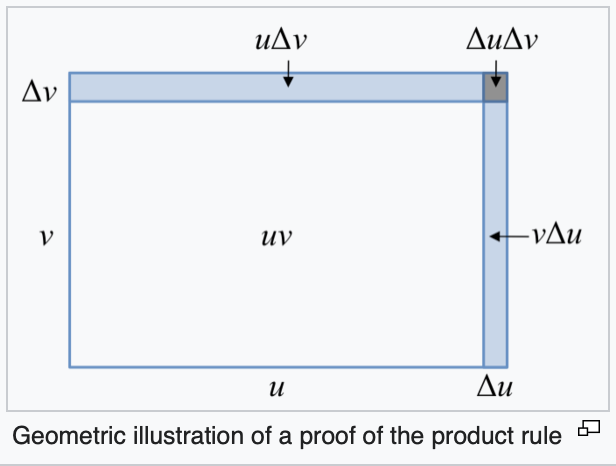
\includegraphics[height=7cm,width=10cm]{product rule.png}
\end{mdframed}
\label{11}
\begin{theorem}
\textbf{(Product Rule and Quotient Rule for Real to Real Function)} Suppose $f$ and $g$ is differentiable at  $x$, and $g'(x)\neq 0$. We have 
\label{3}
\begin{enumerate}[label=(\alph*)]
  \item $(fg)'(x)=f'(x)g(x)+f(x)g'(x)$ (Product Rule)
  \item $(\frac{f}{g})'(x)=\frac{f'(x)g(x)-f(x)g'(x)}{\big(g(x) \big)^2}$ (Quotient Rule)
\end{enumerate}
\end{theorem}
\begin{proof}
Compute 
\begin{align*}
  (fg)'(x)&=\lim_{h\to_0} \frac{f(x+h)g(x+h)-f(x)g(x)}{h}\\
          &=\lim_{h\to 0} \frac{f(x+h)g(x+h)-f(x)g(x+h)+f(x)g(x+h)-f(x)g(x)}{h}\\
          &=\lim_{h\to0} \big(g(x+h) \big) \frac{f(x+h)-f(x)}{h} + \big(f(x) \big) \frac{g(x+h)-g(x)}{h}\\
          &=g(x)f'(x)+f(x)g'(x)
\end{align*}
Compute 
\begin{align*}
  (\frac{f}{g})'(x)&=\lim_{h\to0} \frac{\frac{f(x+h)}{g(x+h)}-\frac{f(x)}{g(x)}}{h}\\
  &=\lim_{h\to0} \frac{f(x+h)g(x)-f(x)g(x+h)}{h g(x+h)g(x)}\\
  &=\lim_{h\to0}\big(\frac{1}{g(x+h)g(x)} \big)\cdot \big(\frac{f(x+h)g(x)-f(x)g(x)+f(x)g(x)-f(x)g(x+h)}{h} \big)\\
  &=\lim_{h\to 0} \Big(\frac{1}{g(x+h)g(x)} \Big) \cdot \Big(\big(g(x) \big) \frac{f(x+h)-f(x)}{h} +\big(f(x) \big) \frac{g(x)-g(x+h)}{h}\Big)\\
  &=\Big(\frac{1}{\big(g(x) \big)^2} \Big)\cdot \Big(\big(g(x)f'(x) \big)-f(x)g'(x) \Big)=\frac{f'(x)g(x)-f(x)g'(x)}{\big(g(x) \big)^2}
\end{align*}
\end{proof}
\begin{mdframed}
  Even a year has past, I can still remember what happened in the first class of Vector Analysis last year. The professor asked: "What is derivative?". A lot of answers emerge, from extremely formal and abstract like $\lim_{h\to 0}\frac{f(x+h)-f(x)}{h}$ to those following geometric intuition like tangent line. Everyone gave a correct answer, but none of them philosophically satisfy the requirement of the question from the professor. Then, he stated: "Derivative is exactly linear approximation", and stated on black board the most general definition:


\end{mdframed}
\begin{definition}
\label{4}
  \textbf{(Definition of Differential)} Given two normed space $V,W$ and an open subset $U\subseteq V$,  we say a function $f:U\rightarrow W$ is \textbf{differentiable at $x$} if there exists a bounded linear operator $A:V\rightarrow W$ such that 
\begin{align*}
\lim_{ h\to 0} \frac{\norm{f(x+h)-f(x)-A(h)}_W}{\norm{h}_V}=0
\end{align*}
and we say the bounded linear map $A$ is the \textbf{(total) derivative} of $f$ at  $x$. 
\end{definition}
\begin{mdframed}
If one put the key words "proof for chain rule" in Google search box, just like the situation in my classes, lots of rigorous proof emerge, but none of them is philosophical satisfying. For this reason, I shall give a proof of chain rule for real to real function based on the concept of linear approximation.\\

In Baby Rudin, derivative of a real to real function $f$ is defined by 
\begin{align*}
f'(a)=\lim_{h\to 0}\frac{f(a+h)-f(a)}{h}
\end{align*}
Immediately from this definition, we can derive a linear approximation $P$ of $f$ at $a$ by setting 
\begin{align*}
P(x)=f(a)+f'(a)(x-a)
\end{align*}
Then, we see if we set $R(x)=f(x)-P(x)$ as the error (or the remainder) of the approximation, then trivially we have the behavior
\begin{align*}
R(x)\to 0\text{ as $x\to a$ }
\end{align*}
what behavior of $R(x)$ that give $P$ the name approximation is 
\begin{align*}
\frac{R(x)}{x-a}\to 0\text{ as }x\to a
\end{align*}
The difference between the two behaviors is symbolically apparent, yet without geometric help, it may be difficult to precisely describe how insignificant the first behavior is compared to the second behavior. For this, observe that any function $g$ that converge to  $f(a)$ at $a$ satisfy the first behavior, yet only a few satisfy the second. One can easily verify that the only linear $\R$ to  $\R$ function that satisfy the second behavior is  $P(x)=f(a)+f'(a)(x-a)$. Geometrically, this means that $R(x)=o(f'(x)dx)$ as $x \to a$.
\label{12}
\end{mdframed}
\begin{theorem}
\textbf{(Chain Rule for $\R$ to $\R$ function)} Suppose $g$ is differentiable at  $a$ and  $f$ is differentiable at  $g(a)$. We have 
\begin{align*}
  (f\circ g)'(a)=f'(g(a))g'(a)
\end{align*}
\end{theorem}
\begin{proof}
Define the remainders $R_{f(g(a))}(x)$ and $R_{g(a)}(x)$ by 
\begin{align*}
\begin{cases}
R_{f(g(a))}(x)=f(x)-f(g(a))-f'(g(a))(x-g(a))\\
R_{g(a)}(x)=g(x)-g(a)-g'(a)(x-a)
\end{cases}
\end{align*}
Compute 
\begin{align}
\label{3.13}
  (f\circ g)'(a)&=\lim_{ x\to a}\frac{f(g(x))-f(g(a))}{x-a}\\
  &=\lim_{x\to a}\frac{R_{f(g(a))}(g(x))+f'(g(a))(g(x)-g(a))}{x-a}
\end{align}
Notice that because $x \to a \implies g(x)\to g(a)$, we have 
\begin{align}
\label{3.12}
\lim_{x\to a} \frac{R_{f(g(a))}(g(x))}{x-a}=\lim_{ x\to a} \frac{R_{f(g(a))}(g(x))}{g(x)-g(a)}\cdot \frac{g(x)-g(a)}{x-a}=0\cdot g'(x)=0
\end{align}
Notice that the above deduction (\myref{Equation}{3.12}) is quite informal for two reasons: First, it may happen that $g(x)=g(a)$ locally. Second, for some reader it may require a mini proof to verify that $\frac{R_{f(g(a))}(g(x))}{g(x)-g(a)}\to 0$ as $x\to a$. These two obstacles for advanced readers should be insignificant.\\

Getting back to \myref{Equation}{3.13}, by \myref{Equation}{3.12}, we now see 
\begin{align*}
  (f\circ g)'(a)=\lim_{x\to a}\frac{f'(g(a))(g(x)-g(a))}{x-a}=f'(g(a))g'(a)
\end{align*}
which finish the proof.
\end{proof}
\section{IVT, EVT and MVT}
\begin{mdframed}
  If one wish to understand most of the Theorems after this section, one must first know MVT, for what an important role it cast in the sections after. Logically prior to MVT is IVT. Yet, unlike MVT involve the intrinsic nature of field and limit structure of $\R$. IVT can be considered as purely topological in the sense that its proof can be stated almost in the language of topology. There are only two facts (the first are purely topological and the second is very close to purely topological) one need to know to prove IVT.\\

First, continuous functions map a connected sets to  connected set. Second, a set in $\R$ is connected if and only if it is an interval.\\

Combining the above two facts, we have the following statement:  
\label{13}
\end{mdframed}
\label{5}
\begin{theorem}
\textbf{(Continuous Real to Real Function Maps Interval to Interval)} as titled.
\end{theorem}
\begin{proof}
Consider the fact a continuous function map connected sets to connected sets and the fact a set in $\R$ is connected if and only if it is an interval.
\end{proof}
\begin{mdframed}
\label{14}
Then, given the necessary constraint (the interval considered is compact) to give the conclusion, we have the famous statement:
\label{6}
\end{mdframed}
\begin{theorem}
\textbf{(IVT)} Given a continuous function $f:[a,b]\to \R$, for each $y$ that lies between $f(a)$ and $f(b)$, there exists $x \in [a,b]$ such that $f(x)=y$.
\end{theorem}
\begin{mdframed}
Given the simplicity of the logical deduction, we shall not give a rigorous proof here. However, one can notice that the interval considered in IVT "must be" compact, otherwise the Theorem is invalid. This constraint is in some sense a showcase how the concept of compact really match  the description of "smallness (bounded) and rigidness (closed)". \\
\label{15}

\label{7}
Compared to IVT, another famous MVT is richer in both the results and the proof. Clearly for a logical and economic purpose, we shall first prove the Cauchy MVT.

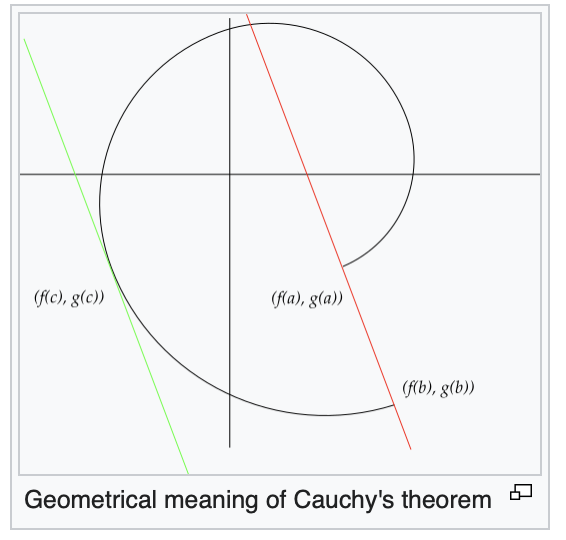
\includegraphics[height=7cm,width=10cm]{CMVT.png}
\end{mdframed}
\begin{theorem}
\label{CMVT}
\textbf{(Cauchy's MVT)} Given a function $f:[a,b]\to \R$ such that  
\begin{enumerate}[label=(\alph*)]
  \item $f,g$ are  differentiable on $(a,b)$
  \item $f,g$ are continuous on $[a,b]$
\end{enumerate}
There exists $x \in (a,b)$ such that 
 \begin{align*}
   \big[f(b)-f(a) \big]g'(x)=\big[g(b)-g(a) \big]f'(x)
\end{align*}
\end{theorem}
\begin{proof}
We wish to find $x \in (a,b)$ such that  
\begin{align*}
\vi{\big[f(b)-f(a)]g'(x)-[g(b)-g(a)]f'(x)=0}
\end{align*}
Define $h$ on  $(a,b)$ by 
\begin{align*}
h(x)=\big[f(b)-f(a)\big]g'(x)-\big[g(b)-g(a)\big]f'(x)
\end{align*}
We reduced our problem into finding $x \in (a,b)$ such that 
\begin{align*}
\vi{h(x)=0}
\end{align*}
Because $f,g$ are both differentiable on  $(a,b)$, we know there exists an anti-derivative $H$ of  $h$ on  $(a,b)$ such that
\begin{align*}
H(x)=\big[f(b) -f(a)\big]g(x)-\big[g(b)-g(a) \big]f(x)
\end{align*}
We have $h=H'$ on  $(a,b)$. This let us reduce our problem into 
\begin{align*}
  \vi{\text{ finding a local extremum of $H$ on  $(a,b)$ }}
\end{align*}
Because $f,g$ are both continuous  on  $[a,b]$, we know $H$ is continuous on $[a,b]$. Then by EVT, we know 
 \begin{align*}
\exists x \in [a,b] , H(x)=\max_{t \in [a,b]}H(t)\text{ and }\exists y \in [a,b], H(y)=\min_{t \in [a,b]}H(t)
\end{align*}
If such $x,y$ is in $(a,b)$, we are done. If not, says that $x,y$ both are on end points $a$ or  $b$. Compute that 
\begin{align*}
H(a)=f(b)g(a)-g(b)f(a)=H(b)
\end{align*}
We see $H$ is constant on  $[a,b]$. Then all points in $(a,b)$ are extremums. $\vdone$
\end{proof}
\begin{corollary}
\label{MVT}
\textbf{(Lagrange's MVT)} Given a function $f:[a,b]\rightarrow \R$ such that 
\begin{enumerate}[label=(\alph*)]
  \item $f$ is differentiable on  $(a,b)$ 
  \item $f$ is continuous on  $[a,b]$
\end{enumerate}
Then there exists $x \in (a,b)$ such that 
\begin{align*}
f'(x)=\frac{f(b)-f(a)}{b-a}
\end{align*}
\end{corollary}
\begin{proof}
Let $g(x)=x$ in Cauchy's MVT (\myref{Theorem}{CMVT}), and we are done.
\end{proof}
\begin{mdframed}
There are two hypotheses in Lagrange's MVT 
\begin{enumerate}[label=(\alph*)]
  \item $f$ is differentiable on $(a,b)$ 
  \item $f$ is continuous on $[a,b]$
\end{enumerate}
They are all necessary. The necessity of differentiablity on $(a,b)$ is clear as shown by the canonical example using absolute value. The necessity of continuity on $[a,b]$ can be shown by the example 
\begin{align*}
f(x)=\begin{cases}
  1& \text{ if $a<x\leq b$ }\\
  0& \text{ if  }x=a
\end{cases}
\end{align*}
\end{mdframed}
\begin{theorem}
\textbf{(First Mean Value Theorem for Definite Integral)} Given a function $f:[a,b]\rightarrow \R$ such that 
\begin{enumerate}[label=(\alph*)]
  \item $f$ is continuous on $(a,b)$
\end{enumerate}
There exists $\xi \in (a,b)$ such that 
\begin{align*}
\int_a^b f(x)dx = f(\xi)\cdot (b-a)
\end{align*}
\end{theorem}
\begin{proof}
We wish 
\begin{align*}
\vi{\text{ to find  }\xi \in (a,b)\text{ such that }f(\xi)=\frac{\int_a^b f(x)dx}{b-a}}
\end{align*}
Define $\tilde{f}:[a,b]\rightarrow \R$ on $[a,b]$ by 
\begin{align}
\label{M1}
\tilde{f}(x)=\begin{cases}
  f(x)& \text{ if $x \in (a,b)$ }\\
  \lim_{t\to a}f(t)& \text{ if $x=a$ }\\
  \lim_{t\to b}f(t)& \text{ if $x=b$ }
\end{cases}
\end{align}
Then, because $\int_a^b f(x)dx=\int_a^b \tilde{f}(x)dx $, we reduce our problem into  
\begin{align*}
\vi{\text{ finding $\xi\in(a,b)$ such that $\tilde{f} (\xi)= \frac{\int_a^b \tilde{f}(x)dx }{b-a}$ }}
\end{align*}
Because $\tilde{f} $ is continuous on $[a,b]$ by definition \myref{Equation}{M1}, by EVT, we know we there exists $\alpha,\beta  \in [a,b]$ such that 
\begin{align}
\label{M4}
\tilde{f} (\alpha )=\inf_{x \in [a,b]}\tilde{f}(x)\text{ and } \tilde{f}(\beta ) =\sup_{x \in[a,b]}\tilde{f}(x) 
\end{align}
WOLG, suppose $\alpha \leq \beta $. Deduce 
\begin{align*}
\tilde{f}(\alpha )= \inf_{x \in [a,b]}\tilde{f}(x)\leq \frac{\int_a^b \tilde{f}(x)dx }{b-a} \leq \sup_{x \in [a,b]}\tilde{f}(x) =\tilde{f}(\beta ) 
\end{align*}
by IVT, we then know there exists $\xi\in [\alpha ,\beta ]$ such that 
\begin{align}
\label{M3}
\exists \xi\in [\alpha ,\beta ], \tilde{f}(\xi)=\frac{\int_a^b \tilde{f}(x)dx }{b-a} 
\end{align}
If $a<\alpha $ and $\beta <b$, our proof is done.\\


If not, notice that if $\tilde{f}(\alpha )=\tilde{f}(\beta )$, then by definition of $\alpha ,\beta $ (\myref{Equation}{M4}), the proof is trivial since $\tilde{f}$ is a constant, so we only have to consider when $\tilde{f}(\alpha )<\tilde{f}(\beta )  $, and we wish to show
\begin{align*}
\vi{\xi \text{ can not happen at $a$ nor $b$ }}
\end{align*}
\As{$\xi=a $, WOLG}. Because $\xi \in [\alpha ,\beta ]$, we know $\alpha =a$. Because $\tilde{f}(\beta )>\tilde{f}(\alpha )  $, we can find $\delta $ such that 
\begin{align}
\label{M5}
\inf_{x \in [\beta  -\delta, \beta  ]}\tilde{f}(x)\geq \frac{\tilde{f}(\alpha )+2\tilde{f}(\beta )  }{3}
\end{align}
We then from \myref{Equation}{M3} see that 
\begin{align}
\label{M6}
\int_a^b \tilde{f}(x)dx=\tilde{f}(\xi)(b-a)=\tilde{f}(\alpha ) (b-a)
\end{align}
Also, we see from definition of $\alpha $ (\myref{Equation}{M4}) and \myref{Equation}{M5} that 
\begin{align}
\int_a^b \tilde{f}(x)dx&=\int_a^{\beta -\delta} \tilde{f}(x)dx + \int_{\beta -\delta}^{\beta  } \tilde{f}(x)dx+\int_{\beta }^{b}\tilde{f}(x)dx \\
&\geq (b -\delta -a) \tilde{f}(\alpha ) + \delta \cdot  \big( \frac{\tilde{f}(\alpha )+2\tilde{f}(\beta )  }{3}\big)\\
&> (b -\delta -a) \tilde{f}(\alpha ) + \delta \cdot  \big( \frac{\tilde{f}(\alpha )+\tilde{f}(\beta )  }{2}\big)\\
&=\tilde{f}(\alpha ) \big(b-a-\frac{\delta}{2} \big) + \tilde{f}(\beta ) \cdot \big( \frac{\delta}{2}\big)
 \label{M7}
\end{align}
Now, from \myref{Equation}{M6} and \myref{Equation}{M7}, we can deduce  
\begin{align*}
\tilde{f}(\alpha )(b-a)> \tilde{f}(\alpha )(b-a-\frac{\delta}{2}) +\tilde{f}(\beta ) \cdot \big(\frac{\delta}{2} \big)
\end{align*}
Then we can deduce
\begin{align*}
\tilde{f}(\alpha )\cdot \big(\frac{\delta}{2} \big)>\tilde{f}(\beta )\cdot \big(\frac{\delta}{2} \big) \tCaC \vdone
\end{align*}
\end{proof}
\begin{theorem}
\textbf{(Second Mean Value Theorem for Definite Integral)} Given functions $G,\phi :[a,b]\rightarrow \R$ such that 
\begin{enumerate}[label=(\alph*)]
  \item $G$ is monotonic
  \item $\phi$ is Riemann-Integrable
\end{enumerate}
Let $G(a^+)=\lim_{t\to a^+}G(t)$ and $G(b^-)=\lim_{t\to b^-}G(t)$. Then there exists $\xi \in (a,b)$ such that 
\begin{align*}
\int_a^b G(t)\phi (t)dt= G(a^+)\int_a^{\xi} \phi(t)dt+G(b^-)\int_\xi^{b}\phi (t)dt
\end{align*}
\end{theorem}
\begin{proof}
Define $f$ on  $[a,b]$ by 
\begin{align*}
f(x)=G(a^+)\int_a^x \phi(t)dt+G(b^-)\int_x^b \phi(t)dt
\end{align*}
We then reduce the problem into 
\begin{align*}
\vi{\text{ finding }\xi \in (a,b)\text{ such that }\int_a^b G(t)\phi (t)dt=f(\xi)}
\end{align*}
By \myref{Theorem}{FTC1}, we know $f$ is continuous on  $[a,b]$. Then by IVT, we can reduce the problem into 
\begin{align*}
\vi{\text{ finding an interval $[c,d]\subseteq (a,b)$ such that }\int_a^b G(t)\phi (t)}\text{ is between $f(c) $ and $f(d)$ }
\end{align*}


Observe that 
\begin{align*}
f(a)=G(b^-)\int_a^b \phi(t)dt\text{ and }f(b)=G(a^+)\int_a^b \phi(t)dt 
\end{align*}




\end{proof}




\section{Riemann-Stieltjes on Computation}
\begin{theorem}
\label{CoV}
\textbf{(Change of Variable)} Given two functions $g,\beta  :[A,B]\rightarrow \R$, a function $\phi: [A,B]\rightarrow [a,b]$ and two functions $f,\alpha :[a,b]\rightarrow \R$ such that 
\begin{enumerate}[label=(\alph*)]
  \item $g = f \circ  \phi $ for all $x \in [a,b]$
  \item $\beta = \alpha  \circ \phi $ for all $x \in [a,b]$ 
  \item $\alpha , \beta  $ increase respectively on $[a,b]$ and $[A,B]$ 
  \item $\phi:[A,B]\rightarrow [a,b]$ is a homeomorphism 
  \item $\int_a^b fd\alpha $ exist
\end{enumerate}
Then 
\begin{align*}
\int_A^B g d\beta  =\int_a^b fd\alpha \text{   (This implies $\int_A^B gd\beta $ exists)}
\end{align*}
\end{theorem}          
\begin{proof}
Fix $\epsilon $. We only wish 
\begin{align*}
  \vi{\text{ to find a partition $Q$ of  $[A,B]$ &such that $U(Q,g,\beta )-L(Q,g,\beta )<\epsilon  $  }}\\
  \vi{\text{ and such that $\int_a^b fd\alpha \in \Big[L(Q,g,\beta ),U(Q,g,\beta ) \Big]$  }}
\end{align*}
Because $\int_a^b fd\alpha $ exists, we know 
\begin{align}
\label{CR1}
\text{ there exists a partition $P$ of  $[a,b]$ such that }U(P,f,\alpha )-L(P,f,\alpha )<\epsilon 
\end{align}
where, of course, $\int_a^b fd\alpha  \in \Big[L(P,f,\alpha ),U(P,f,\alpha )\Big]$.\\

Let $P=\set{a=x_0,x_1,\dots ,x_n=b}$. Because $\phi$ is a homeomorphism, we can let $\phi$ be strictly increasing WOLG.\\ 

Define a partition $Q$ on  $[A,B]$ by 
\begin{align*}
Q=\phi^{-1}[P]=\set{A=\phi^{-1}(x_0),\phi^{-1}(x_1),\dots ,\phi^{-1}(x_n)=B}
\end{align*}
Now, because $\beta =\alpha \circ  \phi$ and $g=f\circ \phi$  for all $x\in [a,b]$ by premise, and because $\phi$ is a homeomorphism, we have 
\begin{align}
  U(Q,g,\beta )&=\sum_{k=1}^n \big[  \sup_{t \in [\phi^{-1}(x_{k-1}),\phi^{-1}(x_k)]} g(t)\big] \big[\beta (\phi^{-1}(x_{k})) - \beta  (\phi^{-1}(x_{k-1}))\big]\notag\\
  &=\sum_{k=1}^n  \big[  \sup_{t \in [\phi^{-1}(x_{k-1}),\phi^{-1}(x_k)]} f \circ  \phi (t)\big] \big[\alpha \circ \phi  \big(\phi^{-1}(x_{k})\big) - \alpha \circ \phi \big(\phi^{-1}(x_{k-1})\big)\big]\notag\\
  &=\sum_{k=1}^n \big[\sup_{t \in [x_{k-1},x_k]}f(t) \big] \big(\alpha (x_k)-\alpha (x_{k-1}) \big)=U(P,f,\alpha )
\label{CR2}
\end{align}
Similarly, we can deduce $L(Q,g,\beta )=L(P,f,\alpha )$. Now, from \myref{Equation}{CR2} and by definition of $P$ (\myref{Equation}{CR1}), we see 
\begin{align*}
&U(Q,g,\beta )-L(Q,g,\beta )=U(P,f,\alpha )-L(P,f,\alpha )<\epsilon \\
  \text{ and }&\int_a^b fd\alpha \in \Big[L(P,f,\alpha ),U(P,f,\alpha ) \Big]=\Big[ L(Q,g,\beta ),U(Q,g,\beta ) \Big]\vdone
\end{align*}



\end{proof}
\begin{theorem}
\label{RRSI}
\textbf{(Reduction of Riemann-Stieltjes Integral: Part 1)} Given two functions $f,\alpha :[a,b]\rightarrow \R$ such that 
\begin{enumerate}[label=(\alph*)]
  \item $\alpha $ increase on $[a,b]$ 
  \item $\alpha $ is differentiable on $(a,b)$ 
  \item $\lim_{x\to b^-}\frac{\alpha (x)-\alpha (b)}{x-b}$ exists and $\lim_{x\to a^+}\frac{\alpha (x)-\alpha (a)}{x-a}$ exists
  \item $\alpha '$ is properly Riemann-Integrable on $[a,b]$  
  \item $f$ is bounded on  $[a,b]$
\end{enumerate}
Then 
\begin{align*}
\int_a^b fd\alpha \text{ exists }\iff  \int_a^b f(x)\alpha '(x)dx\text{ exists and they equal to each other if exists}
\end{align*}
\end{theorem}
\begin{proof}
We wish to prove 
\begin{align*}  \vi{\overline{\int_a^b}fd\alpha = \overline{\int_a^b} f(x)\alpha '(x)dx}
\end{align*}
Fix $\epsilon $. We reduce the problem into proving 
\begin{align*}  \vi{\abso{\overline{\int_a^b}fd\alpha -\overline{\int_a^b}f(x)\alpha '(x)dx}<\epsilon }
\end{align*}
Then, because for all partition $P$ of  $[a,b]$, we have 
\begin{align*}  &\abso{\overline{\int_a^b}fd\alpha - \overline{\int_a^b}f(x)\alpha '(x)dx}\\
  &\leq \abso{\overline{\int_a^b} fd\alpha -U(P,f,\alpha )}-\Bigg|U(P,f,\alpha )-U(P,f\alpha' )\Bigg|-\abso{U(P,f\alpha' )- \overline{\int_a^b} f(x)\alpha '(x)dx}
\end{align*}
We only wish 
\begin{align*}
\vi{\text{  to find $P$ such that}}&\vi{\abso{\overline{\int_a^b}fd\alpha - U(P,f,\alpha )}<\frac{\epsilon}{3}}\\
\vi{\text{ and }}&\vi{\Bigg|U(P,f,\alpha )-U(P,f\alpha' )\Bigg|<\frac{\epsilon}{3}\text{ and }\abso{\overline{\int_a^b}f(x)\alpha '(x)dx- U(P,f\alpha ')}<\frac{\epsilon}{3}}
\end{align*} 
Because $f$ is bounded on  $[a,b]$, we can let $M=\sup_{x \in [a,b]} \abso{f(x)}$. Because $\int_a^b \alpha' (x)dx$ exists, we can let $P$ satisfy 
 \begin{align}
\label{CR3}
U(P,\alpha ')-L(P,\alpha ')<\frac{\epsilon }{4M}
\end{align}
By definition of Riemann Upper sum, we can further refine $P$ to let $P$ satisfy 
\begin{align*}
\abso{\overline{\int_a^b}fd\alpha -U(P,f,\alpha )}<\frac{\epsilon}{3}\text{ and }\abso{\overline{\int_a^b}f(x)\alpha '(x)dx- U(P,f\alpha ')}<\frac{\epsilon}{3}
\end{align*}
It is clear that the statement concerning $P$  (\myref{Equation}{CR3}) remain valid after refinement of $P$. Fix such $P$. We now have reduced the problem into proving 
\begin{align*}
  \vi{\abso{U(P,f,\alpha )-U(P,f\alpha ')}<\frac{\epsilon}{3}}
\end{align*}
Express $P$ in the form $P=\set{a=x_0,x_1,\dots ,x_n=b}$. By MVT (\myref{Theorem}{MVT}), we know for all $k \in \set{1,\dots ,n}$ there exists $t_k \in [x_{k-1},x_k]$ such that
\begin{align}
\label{CR4}
\Delta \alpha_k=  \alpha' (t_k)\Delta x_k
\end{align}
Then, because $U(P,\alpha ')-L(P,\alpha )'<\frac{\epsilon}{3M}$ (\myref{Equation}{CR3}), we now see 
\begin{align}
  \label{CR5}
\sum_{k=1}^n \abso{\alpha '(s_k)-\alpha '(t_k)} \Delta x_k<\frac{\epsilon}{3M} \text{ if $s_k \in [x_{k-1},x_k]$ for all $k \in \set{1,\dots , n}$ }
\end{align}
Then from \myref{Equation}{CR4}, definition of $M$ and \myref{Equation}{CR5}, we have 
\begin{align*}
\abso{\sum_{k=1}^n f(s_k)\Delta \alpha_k - \sum_{k=1}^n f(s_k)\alpha '(s_k)\Delta x_k}&=\abso{\sum_{k=1}^n f(s_k)\big(\alpha '(s_k)-\alpha '(t_k) \big)\Delta x_k}\\
&\leq \sum_{k=1}^n \abso{f(s_k)}\cdot \abso{\alpha '(s_k)-\alpha '(t_k)}\Delta x_k\\
&\leq M \sum_{k=1}^n \abso{\alpha '(s_k)-\alpha '(t_k)}\Delta x_k \\
&<\frac{\epsilon}{4}
\end{align*}
Then because $\sum_{k=1}^m f(s_k)\alpha '(s_k)\Delta x_k\leq  U(P,f\alpha ')$, we now have 
\begin{align}
\label{CR6}
\sum_{k=1}^n f(s_k)\Delta \alpha_k < U(P,f\alpha ')+\frac{\epsilon}{4}
\end{align}
Because \myref{Equation}{CR6} hold true for all choices of  $s_k$, we have 
\begin{align*}
U(P,f,\alpha )<  U(P,f\alpha ')+\frac{\epsilon}{3}
\end{align*}
Similarly, we can deduce 
\begin{align*}
U(P,f\alpha ')<U(P,f,\alpha )+\frac{\epsilon}{3}\vdone
\end{align*}
\end{proof}
\begin{theorem}
\textbf{(Substitution Law)} Given a function $\phi: [a,b]\rightarrow [A,B]$ and a function $f:[A,B]\rightarrow \R$ such that 
\begin{enumerate}[label=(\alph*)]
  \item $\phi$ is a homoeomorphism. 
  \item $\phi$ is differentiable on $(a,b)$ 
  \item $\int_a^b \phi' (x)dx$ exists.  
  \item $f$ is integrable on  $[A,B]$
\end{enumerate}
We have 
\begin{align*}
\int_a^b f\big(\phi (x) \big)\phi' (x)dx=\int_A^B f(u)du
\end{align*}
\end{theorem}
\begin{proof}
Because $f\circ \phi$ and  $\phi'$ is integrable on $[a,b]$, by reduction of Riemann-Stieljes Integral (\myref{Tehroem}{RRSI}), we know 
\begin{align*}
\int_a^b \big(f\circ \phi)(x)  \phi'(x)dx= \int_a^b \big(f\circ \phi \big)(x)d \phi
\end{align*}
Let $\alpha (x)=x$. Let $\beta = \alpha \circ  \phi$. Define $g=f \circ  \phi $. By Change of Variable (\myref{Theorem}{CoV}), we now have  
\begin{align*}
\int_a^b \big(f \circ  \phi \big)(x)d \phi =\int_a^b g(x)d\beta = \int_A^B f(x)dx
\end{align*}
\end{proof}
\section{Weierstrass approximation Theorem: $[a,b]\rightarrow \R$}
\begin{theorem}
\label{Bernoulli's Inequality}
\textbf{(Bernoulli's Inequality)} Given $r,x \in\R$, suppose 
\begin{enumerate}[label=(\alph*)]
  \item $r\geq 1$ 
  \item $x\geq -1$
\end{enumerate}
Then
\begin{align*}
  (1+x)^r\geq 1+rx
\end{align*}
\end{theorem}
\begin{proof}
Fix $r\geq 1$. We wish 
\begin{align*}
\vi{\text{ to prove }(1+x)^r\geq 1+rx\text{ for all  }x \geq -1}
\end{align*}
Define $f:[-1,\infty)\rightarrow \R$ by 
 \begin{align}
\label{Bere1}
f(x)=(1+x)^r-(1+rx)
\end{align}
We reduced the problem into  
\begin{align*}
\vi{\text{ proving }f(x)\geq 0\text{ for all } x\geq -1}
\end{align*}
Because $r\geq 1$ by premise, by definition of $f(x)$  (\myref{Equation}{Bere1}), we see that 
\begin{align*}
f(0)=0\text{, and }f(-1)=r-1\geq 0
\end{align*}
Notice that by definition of $f$  (\myref{Equation}{Bere1}),  $f(x)$ is clearly differentiable on $(-1,\infty)$.\\

Then, by MVT (\myref{Theorem}{MVT}), to prove $f(x)\geq 0$ on $(-1,\infty)$, we only wish 
\begin{align*}
\vi{\text{ to prove }f'(x)\geq 0\text{ for all }x> 0\text{ and }f'(x)\leq 0\text{ for all $x \in (-1,0)$ }}
\end{align*}
Compute $f'$
 \begin{align*}
f'(x)&=r(1+x)^{r-1}-r\\
&=r\Big((1+x)^{r-1}-1 \Big)
\end{align*}
Because $r\geq 1$, we can deduce 
\begin{align*}
x>0 \implies (1+x)^{r-1}\geq 1 \implies f'(x)=r\Big((1+x)^{r-1}-1 \Big)\geq 0
\end{align*}
and deduce 
\begin{align*}
x \in (-1,0) \implies 1+x \in (0,1) \implies (1+x)^{r-1}\leq 1 \implies f'(x)=r\Big((1+x)^{r-1}-1 \Big)\leq  0
\end{align*}
$\vdone$
\end{proof}
\begin{mdframed}
In this section, notation  $\mathcal{C}\big([a,b] \big)$ means the set of \textbf{real-valued continuous function on $[a,b]$}.
\end{mdframed}
\begin{theorem}
\textbf{(Weierstrass approximation Theorem: $[a,b]\rightarrow \R$)} Let $\R[x]\big|_{[a,b]}$ be the space of polynomials on $[a,b]$ with real coefficient. We have 
\begin{align*}
\text{ $\R[x]\big|_{[a,b]}$ is dense in $\Big(\mathcal{C}\big([a,b] \big),\norm{\cdot}_{\infty} \Big)$ }
\end{align*}
\end{theorem}
\begin{proof}
WOLG, we can let $[a,b]=[0,1]$. The reason we can assume such is explained at last. Now, let $f:[0,1]\rightarrow \R$ be a continuous function. Fix $\epsilon $. We only wish 
\begin{align*}
\vi{\text{ to find $P \in \R[x]\big|_{[0,1]}$ such that $\norm{f-P}_{\infty}<\epsilon $}}
\end{align*}
Define $\tilde{f} \in \mathcal{C}\big([0,1] \big)$ by 
\begin{align}
  \label{tse1}
\tilde{f}(x)= f(x)-f(0)-x \big[f(1)-f(0) \big] 
\end{align}
It is easy to check $\tilde{f}$ is continuous. We first prove that 
\begin{align*}
\blue{\big( \tilde{f}(x)-f(x)\big)\in \R[x]\big|_{[0,1]}  }
\end{align*}
By definition of $\tilde{f} $ (\myref{Equation}{tse1}), we see 
\begin{align*}
\tilde{f}(x)-f(x)=(f(0)-f(1))x- f(0)\in \R[x]\big|_{[0,1]}\bdone
\end{align*}
This reduce our problem into 
\begin{align*}
\vi{\text{ finding }P\in \R[x]\big|_{[0,1]}\text{ such that $\norm{\tilde{f}-P}_{\infty}<\epsilon $ }}
\end{align*}
Notice that by definition of $\tilde{f}$ (\myref{Equation}{tse1}), we have 
\begin{align*}
\tilde{f}(0)=0=\tilde{f}(1) 
\end{align*}
Then, we can expand the definition of $\tilde{f} $  by
\begin{align}
\label{tse2}  
\tilde{f}(x)=\begin{cases}
  \tilde{f} (x)& \text{ if $x\in [0,1]$ }\\
  0& \text{ if $x \not \in [0,1]$ }
\end{cases}
\end{align}
This makes $\tilde{f}$ uniformly continuous on $\R$, since  $\tilde{f}$ is uniformly continuous on $[0,1]$ and $[0,1]^c$. Now, for each $n\inn$, define $Q_n \in \R[x]$ by 
\begin{align}
\label{tse3}
Q_n=c_n(1-x^2)^n\text{ where $c_n$ is chosen to satisfy }\int_{-1}^1 Q_n(x)dx=1
\end{align}
Define $P_n:[0,1]\rightarrow \R$ by 
\begin{align*}
P_n(x)=\int_{-1}^1 \tilde{f} (x+t)Q_n(t)dt
\end{align*}
We now prove 
\begin{align*}
\olive{P_n \in \R[x]\big|_{[0,1]}}
\end{align*}
Because $\tilde{f}(x)=0$ for all $x \not \in (0,1)$ by definition of $\tilde{f} $ (\myref{Equation}{tse2}), we see that 
\begin{align}
\label{tse4}
P_n(x)=\int_{-x}^{1-x}\tilde{f}(x+t)Q_n(t)dt \text{ for all }x \in [0,1]
\end{align}
Fix $x \in [0,1]$. Now, by change of variable, we see 
\begin{align*}
P_n(x)=\int_{-x}^{1-x} \tilde{f}(x+t)Q_n(t)dt=\int_{0}^1 \tilde{f}(u)Q_n(u-x)du  
\end{align*}
Because $Q_n$ is a polynomial by definition (\myref{Equation}{tse3}), we can express $Q_n(u-x)$ by 
\begin{align*}
Q_n(u-x)=\sum_{k=0}^{m} a_k x^k\text{ for some $\set{a_0,\dots ,a_m}$ depending on $u$}
\end{align*}
Then we see 
\begin{align*}
  P_n(x)=\int_0^1 \tilde{f}(u)Q_n(u-x)du= \sum_{k=0}^m x^k \Big( 
\int_0^1 \tilde{f}(u) a_kdu
  \Big)  
\end{align*}
This shows that $P_n \inr[x]\big|_{[0,1]}$

$\odone$\\


Now, because $\tilde{f}$ is uniformly continuous on $\R$, we can fix $\delta<1$ such that 
\begin{align}
\label{tse5}
\forall x,y \inr, \abso{x-y}<\delta \implies \abso{\tilde{f}(x)-\tilde{f}(y)  }<\frac{\epsilon}{2}
\end{align}
By definition of $\tilde{f}$ (\myref{Equation}{tse2}), we know $\tilde{f} $ is a bounded function. Then we can set $M$ by 
\begin{align*}
M=\sup_{x \inr} \abso{f(x)}
\end{align*}
Let $n$ satisfy 
 \begin{align}
  \label{tse5}
4M \sqrt{n} (1-\delta^2)^n < \frac{\epsilon}{2} 
\end{align}
Such $n$ exists, because  $\delta<1 \implies  \sqrt{n}(1-\delta^2)^n \to 0 $. We claim 
\begin{align*}
\vi{\text{ $P_n$ satisfy $\norm{\tilde{f}-P_n}_{\infty}<\epsilon $}}
\end{align*}
We first prove 
\begin{align*}
\blue{c_n< \sqrt{n} }
\end{align*}
By Bernoulli's Inequality (\myref{Theorem}{Bernoulli's Inequality}). Compute 
\begin{align*}
1=\int_{-1}^1 Q_n(x)dx&=  c_n\int_{-1}^1 (1-x^2)^n dx \\
&=2c_n\int_0^1 (1-x^2)^n dx\\
&\geq 2c_n\int_0^{\frac{1}{\sqrt{n} }}(1-x^2)^n dx\\
&\geq 2c_n \int_0^{\frac{1}{\sqrt{n} }} 1-nx^2dx=c_n\big(\frac{4}{3\sqrt{n} } \big)> c_n (\frac{1}{\sqrt{n} })
\end{align*}


This implies 
\begin{align*}
\sqrt{n}>c_n \bdone
\end{align*}
Because $\sqrt{n}>c_n $, by definition of $Q_n$  (\myref{Equation}{tse3}), we have 
\begin{align*}
Q_n(x)<\sqrt{n}(1-x^2)^n \leq \sqrt{n}(1-\delta^2)^n \text{ for all $x$ such that  $\delta \leq \abso{x}\leq 1$ }
\end{align*}
Fix $x \in [0,1]$. Finally, because 
\begin{enumerate}[label=(\alph*)]
  \item $\int_{-1}^1 Q_n(x)dx=1$ by definition of  $Q_n$  (\myref{Equation}{tse3})
  \item $Q_n(x)=c_n(1-x^2)^n\geq 0$ for all $x \in [-1,1]$ 
  \item $\abso{\tilde{f}(x+t)-\tilde{f}(x)}<\frac{\epsilon}{2} $ for all $t$ such that $\abso{t}<\delta $, by definition of $\delta $ (\myref{Equation}{tse5})
  \item $Q_n(x)\leq \sqrt{n}(1-\delta^2)^n $ for all $x$ such that  $\delta\leq \abso{x}\leq 1$
  \item $4M\sqrt{n}(1-\delta^2)^n<\frac{\epsilon}{2} $ by definition of $n$  (\myref{Equation}{tse5})
\end{enumerate}
we have
\begin{align*}
\abso{P_n(x)-\tilde{f}(x)}&=\abso{\int_{-1}^1 \tilde{f}(x+t)Q_n(t)dt- \tilde{f}(x)}\\
&=\abso{\int_{-1}^1 \tilde{f}(x+t)Q_n(t)dt- \tilde{f}(x)\int_{-1}^1 Q_n(t)dt }\\
&=\abso{\int_{-1}^1 \tilde{f}(x+t)Q_n(t)dt -\int_{-1}^1 \tilde{f}(x)Q_n(t)dt}\\
&=\abso{\int_{-1}^1 \big[\tilde{f}(x+t)-\tilde{f}(x)   \big]Q_n(t)dt}\\
&\leq \int_{-1}^1 \abso{\big[ \tilde{f}(x+t)-\tilde{f}(x)\big]Q_n(t)}dt\\
&=\int_{-1}^1 \abso{\tilde{f}(x+t)-\tilde{f}(x)  }Q_n(t)dt\\
&\leq \int_{-1}^{-\delta} 2MQ_n(t)dt +\int_{-\delta}^{\delta} \abso{\tilde{f}(x+t)-\tilde{f}(x)  }Q_n(t)dt+\int_{\delta}^1 2M Q_n(t)dt\\
&\leq 2M\Big(\int_{-1}^{-\delta}Q_n(t)dt+\int_{\delta}^1 Q_n(t)dt  \Big)+ \int_{-\delta}^\delta \big(\frac{\epsilon}{2} \big)Q_n(t)dt\\
&\leq 4M(1-\delta) \sqrt{n}(1-\delta^2)^n+ \frac{\epsilon}{2} \\
&\leq 4M\sqrt{n}(1-\delta^2)^n+\frac{\epsilon}{2} <\epsilon  
\end{align*}
Because $x$ is arbitrarily picked from  $[0,1]$, we now have $\norm{P_n-\tilde{f} }_{\infty}<\epsilon \vdone$\\

Lastly, we show 
\begin{align*}
\olive{\text{ our result can be transplanted to arbitrary $\mathcal{C}\big([a,b] \big)$ }}
\end{align*}
Let $[a,b]$ be arbitrary. Fix $\epsilon $ and $f \in \mathcal{C}\big([a,b] \big)$. We wish 
\begin{align*}
\olive{\text{ to find $P \in \R[x]\big|_{[a,b]}$ such that $\norm{f-P}_\infty\leq \epsilon $ }}
\end{align*}
Define $g:[0,1]\rightarrow \R$ by 
\begin{align}
g(x)\triangleq f(a+(b-a)x)
\end{align}
We know there exists $P_n:[0,1]\rightarrow \R$ such that 
\begin{align*}
\norm{P_n-g}_{\infty}<\epsilon 
\end{align*}
Define $H_n:[a,b]\rightarrow \R$ by 
\begin{align*}
H_n(x)=P_n\big(\frac{x-a}{b-a} \big)
\end{align*}
Because $P_n$ is a real polynomial on  $[0,1]$, we know $H_n$ is a real polynomial on $[a,b]$. We now claim 
\begin{align*}
  \olive{\text{ such $H_n\text{ works }$ }}
\end{align*}
Fix $x \in [a,b]$. Observe 
\begin{align*}
\big|f(x)-H_n(x)\big|&=\abso{f(x)-P_n\big(\frac{x-a}{b-a} \big)}\\
&=\abso{g\big(\frac{x-a}{b-a} \big)-P_n\big(\frac{x-a}{b-a} \big)}< \epsilon \odone
\end{align*}
\end{proof}
\begin{mdframed}
It is at now, we will show that every real-valued continuous functions on $[a,b]$ can be approximated by polynomials with rational coefficient. This fact enable our computer to more easily approximate real-valued continuous function on $[a,b]$.\\

Note that since $\mathcal{C}\big([a,b] \big)$ is a separable metric space, we can show that $\mathcal{C}\big([a,b] \big)$ has cardinality of at most continuum $\mathfrak{c}$ . 
\end{mdframed}
\begin{theorem}
\textbf{(The space $\Q[x]|_{[a,b]}$ is dense in $\Big( \mathcal{C}\big([a,b] \big),\norm{\cdot}_{\infty}\Big)$, thus $\mathcal{C}\big([a,b] \big)$ is separable)} 
\begin{align*}
\Big( \mathcal{C}\big([a,b] \big),\norm{\cdot}_{\infty}\Big)\text{ is separable }
\end{align*}
\end{theorem}
\begin{proof}
Because $\Q[x]\big|_{[a,b]}$ is countable, to show $\mathcal{C}\big([a,b] \big)$ is separable, we only wish to show 
\begin{align*}
\vi{\Q [x]\big|_{[a,b]}\text{ is dense in }\mathcal{C}\big([a,b] \big)}
\end{align*}
Because $\R[x]\big|_{[a,b]}$ is dense in $\mathcal{C}\big([a,b] \big)$, we reduce our problem into proving 
\begin{align*}
\vi{\Q[x]\big|_{[a,b]}\text{ is dense in }\R[x]\big|_{[a,b]}}
\end{align*}
Fix $\epsilon \text{ and } P \in \R[x]\big|_{[a,b]}$. We must
\begin{align*}
\vi{\text{ find $Q \in \Q[x]\big|_{[a,b]}$ such that $\norm{Q-P}_\infty \leq \epsilon $}}
\end{align*}
Express $P(x)=\sum_{k=0}^n r_kx^k$. Let $M> \max \set{\abso{a},\abso{b}}$. Because $\Q$ is dense in $\R$, we know there exists $c_k \inq$ such that  $\abso{c_k-r_k}< \frac{\epsilon }{(n+1)M^n}$. We claim 
\begin{align*}
\vi{Q(x)=\sum_{k=0}^n c_kx^k\text{ works }}
\end{align*}
Fix $x \in [a,b]$. See
\begin{align*}
\abso{P(x)-Q(x)}&=\abso{\sum_{k=0}^n (c_k-r_k)x^k}\\
&\leq \sum_{k=0}^n \abso{c_k-r_k}\cdot \abso{x}^k\\
&\leq \sum_{k=0}^n \abso{c_k-r_k}\cdot M^k\\
&\leq (M^n)\sum_{k=0}^n \abso{c_k-r_k}\\
&< M^n (n+1)\big( \frac{\epsilon }{(n+1)M^n}\big)=\epsilon \vdone
\end{align*}
\end{proof}
\section{The Stone-Weierstrass Theorem}
\begin{mdframed}
Recall that a \textbf{vector space over a field $\F$} is a set $V$ equipped with \textbf{vector addition} $+:V\times V\to V$  and \textbf{scalar multiplication}  such that 
\begin{enumerate}[label=(\alph*)]
  \item $(V,+)$ is an abelian group. 
  \item Scalar multiplication is compatible with field multiplication:   $\Big((ab)v=a(bv) \Big)$
  \item Scalar multiplication is distributive: $\Big((a+b)v=av+bv\text{ and }a(v+w)=av+aw \Big)$
\end{enumerate}

There are many ways to define the term \textbf{algebra over a field $\F$}. One can exhaust all the laws an algebra should obey. In short, an \textbf{algebra over a field $\F$} (or \textbf{$\F$-algebra}) is a set $(A,+,\cdot )$ equipped scalar multiplication over $\F$ such that 
\begin{enumerate}[label=(\alph*)]
  \item Multiplication $\cdot $ is $\underline{\text{distributive}}$ with respect to $+$  
  \item $(A,+)$ and scalar multiplication form a vector space. 
   \item Scalar multiplication and vector multiplication $\cdot $ is compatible: $\Big((av)\cdot (bw)=ab(v\cdot w) \Big)$
\end{enumerate}
Given an arbitrary set $E$ and a field $\F$, let $A$ be the set of all functions from  $E$ to $\F$. The following is a list of some algebra 
\begin{enumerate}[label=(\alph*)]
  \item $(\R^3,\text{cross product})$  over $\R$ 
  \item $(\C,\text{complex multiplication})$ over $\C$ 
  \item $(\Q[x],\text{function multiplication})$ over $\Q$
  \item $(\text{Functions from }E\text{ to }\F,\text{function multiplication})$ over $\F$
  \item $(\text{Continuous functions from $(E,\tau)$ to $\C$ },\text{function multiplication})$ over $\C$  
  \item $(\text{Linear transformation from $V$ to $V$, composition})$ over $\F$ where  $V$ is over $\F$
  \item $\big(M_n(\F),\text{matrix multiplication}\big)$ over $\F$
\end{enumerate}
Note that $B=(\text{continuous functions from }\C\text{ to }\C,\text{composition})$ over $\C$ is not an algebra, even though $B$ is both a vector space and a ring. ($\because$ scalar multiplication and multiplication are not compatible).\\

It is at here we shall introduce some general terminologies. Given an arbitrary set $E$, a field  $\F$ and a point $x \in E$, we say a family $\mathcal{F}$ of functions  from $E$ to  $\F$  \textbf{vanish at $x$} if for all $f \in \mathcal{F}$, we have $f(x)=0$. We say $\mathcal{F}$ \textbf{separate points} in $E$ if for all  $x_2\neq x_1 \in E$, there exists $f\in \mathcal{F}$ such that $f(x_2)\neq f(x_1)$. 
\end{mdframed}

\section{FTC}
\begin{theorem}
  \label{FTC1}
\textbf{(Fundamental Theorem of Calculus: Part 1)} Suppose a function $f:[a,\infty )\rightarrow \R$ satisfy
\begin{align*}
f\text{ is $\underline{\text{proper-Riemann integrable}}$ on $[a,b]$  for all $b>a$}
\end{align*}
If we set $F:[a,\infty) \to \R$ 
\begin{align*}
F(x)=\int_a^x f(t)dt
\end{align*}
Then 
\begin{enumerate}[label=(\alph*)]
  \item $F$ is continuous on $[a,\infty )$
  \item $F$ is differentiable at  $x_0 \in [a,\infty )$  where $F'(x_0)=f(x_0)$ if $f$ is continuous at $x_0$
\end{enumerate}
\end{theorem}
\begin{proof}
Fix $\epsilon $ and $[a,b]$. We only wish  
\begin{align*}
\vi{\text{ to prove }F\text{ is continuous on $[a,b]$ }}
\end{align*}
To prove $F$ is continuous on  $[a,b]$, we only wish 
\begin{align*}
\vi{\text{ to find $\delta$ such that $\forall [x,y]\subseteq [a,b], \abso{x-y}<\delta \implies \abso{F(x)-F(y)}<\epsilon $}}
\end{align*}
Because $f $ is proper-Riemann-Integrable on $[a,b]$, we know $f$ is bounded on  $[a,b]$. Let $M$ be an upper bound of  $\abso{f}$ on $[a,b]$. We claim 
\begin{align*}
\vi{\text{ $\delta=\frac{\epsilon}{M}$ works }} 
\end{align*}
Because $y-x <\delta=\frac{\epsilon}{M}$, we have
\begin{align*}
  \abso{F(x)-F(y)}&=\abso{\int_x^y f(t)dt}\\
  &\leq \int_x^y \abso{f(t)}dt\\
  &\leq (y-x)<\epsilon \vdone
\end{align*}
Now, to prove $F'(x_0)=f(x_0)$, we wish 
\begin{align*}
  \blue{\text{ to prove $\lim_{x\to x_0} \frac{F(x)-F(x_0)}{x-x_0}= f(x_0)$ }}
\end{align*}
Fix $\epsilon $. We wish 
\begin{align*}
\blue{\text{ to find $\delta$ such that $\abso{x-x_0}<\delta \implies \abso{\frac{F(x)-F(x_0)}{x-x_0}-f(x_0)}<\epsilon $ }}
\end{align*}
Because $f$ is continuous at $x_0$, we know  
\begin{align}
\label{F1}
\exists \delta, \abso{x-x_0}<\delta \implies \abso{f(x)-f(x_0)}<\epsilon 
\end{align}
We claim 
\begin{align*}
\blue{\text{ such $\delta$ in}}\text{ \myref{Equation}{F1} }\blue{\text{works}}
\end{align*}
WOLG, let $x>x_0$. Deduce 
\begin{align*}
\abso{\frac{F(x)-F(x_0)}{x-x_0}-f(x_0)}&=\abso{\frac{\int_{x_0}^x f(t)dt}{x-x_0}-f(x_0)}\\                  &=\abso{\frac{\int_{x_0}^x \big[f(t)-f(x_0) \big]dt}{x-x_0}}\\
&\leq \frac{\int_{x_0}^x \abso{f(t)-f(x_0)}dt}{\abso{x-x_0}}\\
&\leq \frac{\int_{x_0}^x \epsilon dt}{\abso{x-x_0}}=\epsilon \bdone
\end{align*}
\end{proof}
\begin{theorem}
\label{FTC2}
\textbf{(Fundamental Theorem of Calculus: Part 2, Leibniz Rule)} Suppose two functions $f,F:[a,\infty )\rightarrow \R$ satisfy 
\begin{enumerate}[label=(\alph*)]
  \item $f$ is proper Riemann-Integrable on $[a,b]$ for all $b>a$ 
\item $F'(x)=f(x)$ for all $x \in (a, \infty)$ 
\item $F$ is continuous on  $[a,\infty)$
\end{enumerate}
Then for all $b>a$, 
\begin{align*}
\int_a^b f(x)dx=F(b)-F(a)
\end{align*}
\end{theorem}
\begin{proof}
Fix $\epsilon $. We wish 
\begin{align*}
\vi{\text{ to show that $\abso{\Big( F(b)-F(a)\Big)-\int_a^b f(x)dx}<\epsilon $ }}
\end{align*}
Because $f$ is proper Riemann-Integrable on $[a,b]$, we know there exists a partition $P=\set{a=x_0,x_1,\dots , x_n=b}$ of  $[a,b]$ such that 
\begin{align}
\label{FP}
U(P,f)-L(P,f)<\epsilon 
\end{align}
Because $f=F'$ on  $(a,b)$, for each $k \in \set{1,\dots ,n}$, by MVT (\myref{Theorem}{MVT}), we know 
\begin{align*}
\exists t_k \in (x_{k-1},x_k), \frac{F(x_k)-F(x_{k-1})}{x_k-x_{k-1}}=f(t_k)
\end{align*}
This let us deduce
\begin{align*}
F(b)-F(a)=\sum_{k=1}^n F(x_k)-F(x_{k-1})=\sum_{k=1}^n f(t_k) \Delta x_k
\end{align*}
Now, we have 
\begin{align*}
  \int_a^b f(x)dx\text{ and }F(b)-F(a)\text{ are both in }\big[ L(P,f),U(P,f) \big]
\end{align*}
Then by \myref{Equation}{FP}, we can deduce 
\begin{align*}
\abso{F(b)-F(a)- \int_a^b f(x)dx}<\epsilon \vdone
\end{align*}




\end{proof}
\begin{theorem}
\textbf{(Integral By Part)} Given four function $f,g,F,G:[a,b]\rightarrow \R$ such that 

\begin{enumerate}[label=(\alph*)]
  \item $F'(x)=f(x)\text{ and }G'(x)=g(x)$ for all $x\in (a,b)$ 
  \item $f,g$ are properly Riemann-Integrable on  $[a,b]$ 
  \item $F,G$ are continuous on  $[a,b]$
\end{enumerate}
We have
\begin{align}
\label{FI}
\int_a^b F(x)g(x)dx=FG\Big|^b_a-\int_a^b f(x)G(x)dx
\end{align}
\end{theorem}
\begin{proof}
To prove \myref{Equation}{FI}, we only with 
\begin{align*}
\vi{\text{ to prove }\int_a^b F(x)g(x)dx+\int_a^b f(x)G(x)dx=FG\Big|_a^b}
\end{align*}
We can reduce the problem 
\begin{align*}
\vi{\text{ into proving }\int_a^b \big( Fg+fG \big) dx=FG\Big|_a^b}
\end{align*}
Notice that by Chain Rule,  
\begin{align*}
\big(FG \big)'(x)=F(x)g(x)+f(x)G(x)\text{ for all $x \in (a,b)$ }
\end{align*}
Then the result follows from Part 2 of Fundamental Theorem of Calculus (\myref{Theorem}{FTC2}). $\vdone$
\end{proof}
\begin{Example}{\textbf{(Discontinuous Derivative)}}{}
\begin{align*}
f(x)=\begin{cases}
  \frac{x^2}{\sin x}& \text{ if $x\neq 0$ }\\
  0& \text{ if $x=0$ }
\end{cases}
\end{align*}
\end{Example}
\section{Uniform Convergence on Integration and Differentiation}
\begin{theorem}
\label{RIFac}
\textbf{(Riemann-Integration and Uniform Convergence)} Given a function $\alpha :[a,b]\rightarrow \R$ and a sequence of functions $f_n:[a,b]\rightarrow \R$ such that 
\begin{enumerate}[label=(\alph*)]
  \item $\alpha $ increase on $[a,b]$ 
  \item $\int_a^b f_nd\alpha $ exists for all $n\inn$ 
  \item $f_n \to f $ uniformly on $[a,b]$ 
\end{enumerate}
Then 
\begin{align*}
  \lim_{n\to \infty}\int_a^b f_n d\alpha \text{ exists and }\int_a^b fd\alpha =\lim_{n\to \infty}\int_a^b f_nd\alpha 
\end{align*}
\end{theorem}
\begin{proof}
We first prove 
\begin{align*}
\vi{\int_a^b fd\alpha \text{ exists }}
\end{align*}
Fix $\epsilon $. We wish to prove 
\begin{align*}
\vi{\overline{\int_a^b}fd\alpha - \underline{\int_a^b}fd\alpha < \epsilon }
\end{align*}
Let $\epsilon _n = \norm{f_n-f}_\infty$. Because $f_n \to f$ uniformly, we know 
\begin{align*}
\text{ there exists $n\inn$ such that $\epsilon _n=\norm{f_n-f}_\infty < \frac{\epsilon }{2\big[\alpha (b)-\alpha (a) \big]}$ }
\end{align*}
Because $\alpha $ increase, by definition of $\epsilon _n$, we see 
\begin{align*}
\int_a^b (f_n-\epsilon _n)d\alpha \leq \underline{\int_a^b}fd\alpha \leq \overline{\int_a^b}fd\alpha \leq \int_a^b (f_n+\epsilon_n) d\alpha  
\end{align*}
Because $\epsilon _n <\frac{\epsilon}{2\big[\alpha (b)-\alpha (a) \big]}$, we now see 
\begin{align*}
  \overline{\int_a^b}fd\alpha -\underline{\int_a^b}fd\alpha &\leq \int_a^b (f_n+\epsilon _n)d\alpha -\int_a^b (f_n-\epsilon _n)d\alpha \\
&=\int_a^b (2\epsilon _n)d\alpha<2 \epsilon_n \cdot \big[\alpha (b)-\alpha (a) \big] = \epsilon \vdone
\end{align*}
We now prove 
\begin{align*}
  \blue{\int_a^b f_n d\alpha \to \int_a^b fd\alpha \text{ as $n \to \infty $ }}
\end{align*}
Fix $\epsilon $. We wish 
\begin{align*}
\blue{\text{ to find $N$ such that }\forall n>N,\abso{\int_a^b f_nd\alpha-\int_a^b fd\alpha }<\epsilon  }
\end{align*}
Recall the definition $\epsilon_n= \norm{f_n-f}_\infty$. Because $\epsilon _n \to 0$, we know 
\begin{align}
\label{CuU1}
\text{ there exists $N$ such that }\forall n>N, \epsilon_n < \frac{\epsilon }{\alpha (b)-\alpha (a)}
\end{align}
We claim 
\begin{align*}
\blue{\text{ such $N$ works }}
\end{align*}
Fix $n>N$. From \myref{Equation}{CuU1}, we see
 \begin{align*}
  \abso{\int_a^b f_nd\alpha -\int_a^b fd\alpha }&=\abso{\int_a^b (f_n-f)d\alpha }\\
  &\leq \int_a^b \abso{f_n-f}d\alpha \\
  &\leq \int_a^b \epsilon_n d\alpha =\epsilon_n \big[\alpha (b)-\alpha (a) \big]<\epsilon \bdone
\end{align*}


\end{proof}
\begin{mdframed}
Before the next Theorem, let's see three examples why this time we don't (can't) use the hypothesis: $f_n \to f$ uniformly. 
\begin{Example}{\textbf{(Differentiable functions are NOT closed under uniform convergence)}}{}
\begin{align*}
X=[-1,1]\text{ and }f(x)=\abso{x}
\end{align*}
By Weierstrass approximation Theorem, there is a sequence of polynomials (differentiable) that uniformly converge to $f$, which is not differntiable at  $0$. 
\end{Example}
\begin{Example}{\textbf{(Derivative won't necessarily converge to the right place)}}{}
\begin{align*}
X=\R \text{ and }f_n(x)=\frac{\sin nx}{\sqrt{n} }
\end{align*}
Compute 
\begin{align*}
f'(x)=0 \text{ and }f'_n(x)=\sqrt{n} \cos nx
\end{align*}
\end{Example}
\begin{Example}{\textbf{(Derivative won't necessarily converge to the right place)}}{}
\begin{align*}
X=\R \text{ and }f_n(x)=\frac{x}{1+nx^2}
\end{align*}
Compute 
\begin{align*}
f=\tilde{0} \text{ and }f'_n(0)=1
\end{align*}
\end{Example}
Informally speaking, these examples together with the fact integral are closed under uniform convergence (\myref{Theorem}{RIFac}) should give you some ideas that differentiation and integration although are operations inverse to each other, are NOT symmetric. There is a certain hierarchy on continuous functions on a fixed compact interval. Thus, we have the next Theorem in its form. Note that in application, the next Theorem only require us to prove $f'_n$ uniformly converge, and doesn't require us to prove to where does it converge. 
\end{mdframed}
\begin{theorem}
\label{UCaD}
\textbf{(Uniform Convergence and Differentiation)} Given a sequence of function $f_n:[a,b]\rightarrow \R$ such that 
\begin{enumerate}[label=(\alph*)]
  \item $f'_n$ uniformly converge on  $(a,b)$
  \item $f_n$ are continuous on  $[a,b]$
  \item $f_n(x_0)\to L$ for some $x_0 \in [a,b]$
\end{enumerate}
Then 
\begin{enumerate}[label=(\alph*)]
  \item $f_n$ uniformly converge on  $[a,b]$ 
  \item and
\begin{align*}
\Big(\lim_{n\to \infty}f_n \Big)'(x_0)=\lim_{n\to \infty}f_n'(x_0)\text{ on $(a,b)$ }
\end{align*}
\end{enumerate}
\end{theorem}
\begin{proof}
We first prove 
\begin{align}
\label{fnun}
\vi{f_n\text{ uniformly converge on $[a,b]$}}
\end{align}
Fix $\epsilon $. We wish  
\begin{align*}
  \vi{\text{ to find $N$ such that $\norm{f_n-f_m}_\infty \leq \epsilon $ for all $n,m>N$}}
\end{align*}
Because $f_n(x_0)$ converge, and $f'_n$ uniformly converge, we know there exists $N$ such that 
 \begin{align}
\label{UCD1}
\begin{cases}
 \abso{f_n(x_0)-f_m(x_0)}<\frac{\epsilon}{2} \\
\norm{f_n'-f_m'}_\infty <\frac{\epsilon }{2(b-a)}
\end{cases}\text{ for all $n,m>N$ }
\end{align}
We claim 
\begin{align*}
\vi{\text{ such $N$ works }}
\end{align*}
Fix $x \in [a,b]$ and $n,m>N$. We need
\begin{align*}
  \vi{\text{ to show }\abso{f_n(x)-f_m(x)}\leq \epsilon}
\end{align*}
We first prove
\begin{align*}
\olive{\abso{f_n(x)-f_m(x)-f_n(x_0)+f_m(x_0)}\leq \frac{\epsilon}{2}}
\end{align*}
Because $(f_n-f_m)'=f_n'-f_m'$, by MVT (\myref{Theorem}{MVT}) and \myref{Equation}{UCD1}, we can deduce 
\begin{align*}
 \abso{f_n(x)-f_m(x)-f_n(x_0)+f_m(x_0)}&=\abso{(f_n-f_m)(x)-(f_n-f_m)(x_0)}\\
 &=\Big|\big[(f_n-f_m)'(t)\big](x-x_0)\Big|\text{ for some $t$ between $x,x_0$ }\\
 &< \frac{\epsilon}{2(b-a)}\cdot \abso{x-x_0}\\
 &\leq \frac{\epsilon }{2(b-a)}\cdot (b-a)=\frac{\epsilon}{2}\hspace{0.3cm}\big(\because x,x_0  \in [a,b]\big)\odone
\end{align*}
Now, by \myref{Equation}{UCD1}, we have 
\begin{align*}
  \abso{f_n(x)-f_m(x)}&\leq \abso{f_n(x)-f_m(x)-f_n(x_0)+f_m(x_0)}+\abso{f_n(x_0)-f_m(x_0)}\\
&<\frac{\epsilon}{2}+\frac{\epsilon}{2}=\epsilon \vdone
\end{align*}
We claim 
\begin{align}
\label{UCAC2}
\blue{f(x)\triangleq \lim_{n\to \infty}f_n(x)\text{ satisfy }f'(x)=\lim_{n\to \infty}f'_n(x)\text{ on $(a,b)$ }}
\end{align}
We first show 
\begin{align*}
\olive{f\text{ is differentiable on $(a,b)$ }}
\end{align*}
Fix $x \in (a,b)$. We wish to prove
\begin{align*}
  \olive{{\lim_{t\to x}\frac{f(t)-f(x)}{t-x}\text{ exists }}}
\end{align*}
Define $\phi :[a,b]\setminus x\rightarrow \R$ by 
\begin{align*}
\phi (t)\triangleq \frac{f(t)-f(x)}{t-x}
\end{align*}
We reduce our problem into proving 
\begin{align*}
  \olive{\lim_{t\to x}\phi (t)\text{ exists }}
\end{align*}
Set $\phi_n:[a,b]\setminus x\rightarrow \R$ by 
\begin{align*}
\phi_n(t)\triangleq \frac{f_n(t)-f_n(x)}{t-x}
\end{align*}
We first show  
\begin{align}
\label{UCACu}
  \vi{\phi_n\text{ uniformly converge on }[a,b]\setminus x}
\end{align}
Fix $\epsilon $. We have
\begin{align*}
  \vi{\text{ to find $N$ such that  $\abso{\phi_n(t)-\phi _m(t)}\leq \epsilon $ for all $n,m>N$ and  $t\in [a,b]\setminus x$ }}
\end{align*}
Because $f_n'$ uniformly converge on  $[a,b]$, we know there exists $N$ such that 
 \begin{align}
\label{CUaC1}
\norm{f_n'-f_m'}_\infty\leq \epsilon \text{ for all $n,m>N$ }
\end{align}
We claim 
\begin{align*}
\vi{\text{ such }N\text{ works }}
\end{align*}
Fix $n,m>N$ and $t \in [a,b]\setminus x$. We wish to prove 
\begin{align*}
\vi{\abso{\phi_n(t)-\phi_m(t)}\leq \epsilon }
\end{align*}
Because $(f_n-f_m)'=f_n'-f'_m$, by MVT (\myref{Theorem}{MVT}) and \myref{Equation}{CUaC1}, we can deduce 
\begin{align*}
  \abso{\phi_n(t)-\phi_m(t)}&\leq \abso{\frac{f_n(t)-f_n(x)}{t-x}-\frac{f_m(t)-f_m(x)}{t-x}}\\
                            &=\abso{\frac{\big(f_n-f_m\big)(t)-\big(f_n-f_m\big)(x)}{t-x}}\\
 &=\abso{\big(f'_n-f'_m\big)(t_0)}\text{ for some $t_0$ between $t,x$  }\\
&\leq \epsilon \vdone
\end{align*}
We now show 
\begin{align}
\label{UCACP}
\brown{\phi_n \to \phi\text{ pointwise on $[a,b]\setminus x$}}
\end{align}
Because $f_n \to f$ on $[a,b]$ by definition (\myref{Equation}{UCAC2}), (the convergence is in fact uniform as we have shown. This doesn't matter here tho), for each $t \in [a,b]\setminus x$, we can deduce
\begin{align*}
\lim_{n\to \infty} \phi_n(t)&=\lim_{n\to \infty}\frac{f_n(t)-f_n(x)}{t-x}=\frac{f(t)-f(x)}{t-x}=\phi (t)\bodone
\end{align*}
Now, by \myref{Equation}{UCACu} and \myref{Equation}{UCACP}, we know 
\begin{align*}
\phi_n \to \phi \text{ uniformly on $[a,b]\setminus x$ }
\end{align*}
Notice that because $f_n'(x)$ converge, we know
\begin{align*}
\lim_{n\to \infty}\lim_{t\to x}\phi_n(t)=\lim_{n\to \infty}f'_n(x)\text{ exists }
\end{align*}
Then (Notice that the second equality below hold true because we have known $\lim_{n\to \infty}\lim_{t\to x}\phi_n(t)$ exists), we can finally deduce 
\begin{align*}
\lim_{t\to x}\phi (t)&=\lim_{t\to x}\lim_{n\to \infty}\phi_n(t)\\
&=\lim_{n\to \infty}\lim_{t\to x}\phi_n(t)\\
&=\lim_{n\to \infty}f'_n(x)\text{ exists }\odone
\end{align*}
Now, notice that $f'(x)=\lim_{t\to x}\phi (t)$, so in fact, we have just proved $f'_n \to f'\odone \bdone$



\end{proof}
\begin{mdframed}
As Rudin remarked, a much shorter (and much more intuitive) proof can be given, if we require $f'$ to be continuous on  $[a,b]$. 
\end{mdframed}
\begin{theorem}
\textbf{(Uniform Convergence and Differentiation: Weaker Version)} Given a sequence of function $f_n:[a,b]\rightarrow \R$ such that 
\begin{enumerate}[label=(\alph*)]
  \item $f'_n$ uniformly converge on  $[a,b]$
  \item $f_n(x_0)\to L$ for some $x_0 \in [a,b]$
  \item $f_n$ are of class $C^1$ on $[a,b]$ 
\end{enumerate}

Then 
\begin{enumerate}[label=(\alph*)]
  \item $f_n$ uniformly converge on  $[a,b]$ 
  \item and
\begin{align*}
\frac{d}{dx}\Big(\lim_{n\to \infty}f_n(x) \Big)\Big|_{x=x_0}=\lim_{n\to \infty}f_n'(x_0)\text{ on $(a,b)$ }
\end{align*}
\end{enumerate}
\end{theorem}
\begin{proof}
We claim 
\begin{align*}
  \vi{f(x)=\lim_{n\to \infty}\int_{x_0}^x f'_n(t)dt+L\text{ works }} 
\end{align*}
Note that $\lim_{n\to \infty}\int_{x_0}^x f'_n(t)dt$ exists because $f'_n$ uniformly converge  (\myref{Theorem}{RIFac}).\\

Because $f'_n$ uniformly converge and are continuous on $[a,b]$, by ULT, we know
 \begin{align*}
\int_{x_0}^x \lim_{n\to \infty}f'_n(t)dt+L\text{ exists }
\end{align*}
and know 
\begin{align*}
f(x)=\int_{x_0}^x \lim_{n\to \infty}f'_n(t)dt + L 
\end{align*}
By FTC, we see
 \begin{align*}
f'(x)=\lim_{n\to \infty}f'_n(x)\text{ on }(a,b)
\end{align*}
Such convergence is uniform by premise. To finish the proof, we now only have to prove 
\begin{align*}
\vi{f_n\to f\text{ uniformly on }[a,b]}
\end{align*}
Fix $\epsilon $. We wish 
\begin{align*}
\vi{\text{ to find $N$ such that  $\abso{f_n(x)-f(x)}\leq \epsilon $ for all $n>N$ and  $x \in [a,b]$}}
\end{align*}
Because $f'_n \to f'$ uniformly, and $f_n(x_0) \to L=f(x_0)$ (Check $L=f(x_0)$), we know there exists $N$ such that 
 \begin{align*}
\begin{cases}
  \norm{f'_n-f'}_\infty < \frac{\epsilon }{2(b-a)}\\
  \abso{f_n(x_0)-f(x_0)}<\frac{\epsilon}{2}
\end{cases}\text{ for all $n>N$ }
\end{align*}
We claim 
\begin{align*}
\vi{\text{ such $N$ works }}
\end{align*}
Fix $n>N$ and  $x\in [a,b]$. Observe 
\begin{align*}
\abso{f(x)-f_n(x)}&= \abso{\int_{x_0}^x \big(f'(t)-f'_n(t) \big)dt+f(x_0)-f_n(x_0)}\\
&\leq \int_{x_0}^x \abso{f'(t)-f'_n(t)}dt+ \abso{f(x_0)-f_n(x_0)}\\
&\leq \frac{\epsilon}{2}+\frac{\epsilon}{2}=\epsilon \vdone
\end{align*}
\end{proof}
\section{Fundamental Tests*}
\begin{theorem}
\textbf{(LCT)}
\end{theorem}
\begin{mdframed}

\end{mdframed}
\begin{theorem}
\textbf{(Geometric Series)}
\end{theorem}
\begin{theorem}
\textbf{(p-Series)}
\end{theorem}
\begin{mdframed}

\end{mdframed}
\begin{theorem}
\textbf{(Limit Superior Lemma 1)} 
\begin{align*}
d_n \text{ converge }\implies \limsup_{n\to\infty} c_nd_n=\lim_{n\to \infty}d_n\limsup_{n\to\infty} c_n
\end{align*}
\end{theorem}
\begin{theorem}
\textbf{(Limit Superior Lemma 2)} 
\begin{align*}
\limsup_{n\to\infty} \sqrt[n]{c_n} =\limsup_{n\to\infty} \sqrt[n]{c_{n+k}} 
\end{align*}
\end{theorem}
\begin{mdframed}

\end{mdframed}
\begin{theorem}
\textbf{(Ratio Test)}
\end{theorem}
\begin{theorem}
\textbf{(Root Test)}
\end{theorem}
\begin{theorem}
\textbf{(Root Test is Stronger Than Ratio Test)}
\end{theorem}
\begin{mdframed}

\end{mdframed}
\begin{theorem}
\textbf{(Absolute Convergent Series Converge)}
\end{theorem}
\begin{theorem}
\textbf{(Absolute Convergent Series Unconditionally Converge)}
\end{theorem}
\begin{theorem}
\textbf{(Fubini's Theorem for Infinite Series)}
\end{theorem}
\begin{mdframed}

\end{mdframed}
\begin{theorem}
\textbf{(Summation by Part)}
\end{theorem}
\begin{mdframed}

\end{mdframed}
\begin{theorem}
\textbf{(Alternating Series Test)}
\end{theorem}
\begin{theorem}
\textbf{(Abel's Test)}
\end{theorem}
\begin{theorem}
\textbf{(Dirichlet's Test)}
\end{theorem}
\begin{mdframed}

\end{mdframed}
\begin{theorem}
\label{Merten Cau}
\textbf{(Merten's Theorem for Cauchy Product)} Suppose 
\begin{enumerate}[label=(\alph*)]
  \item $\sum_{n=0}^\infty a_n$ converge absolutely 
  \item $\sum_{n=0}^\infty a_n=A$
  \item $\sum_{n=0}^\infty b_n=B$ 
  \item $c_n=\sum_{k=0}^n a_kb_{n-k}$
\end{enumerate}
Then we have 
\begin{align*}
\sum_{n=0}^{\infty}c_n=AB
\end{align*}
\end{theorem}
\begin{mdframed}

\end{mdframed}
\begin{theorem}
\textbf{(Special Sequence)} $(n!)^{\frac{1}{n}}$
\end{theorem}
\begin{theorem}
\label{WM-t}
\textbf{(Weierstrass M-test)} Given sequences $f_n:X\rightarrow \C$, and suppose 
\begin{align}
\label{K9}
\forall n\inn,\forall x\in X, \abso{f_n(x)}\leq M_n
\end{align}
Then 
\begin{align*}
\sum_{n=1}^\infty M_n\text{ converge }\implies \sum_{n=1}^\infty f_n\text{ uniformly converge }
\end{align*} 
\end{theorem}
\begin{proof}
Because $(\C,\norm{\cdot }_2)$  is complete, by \myref{Corollary}{SoB}, we only wish to prove 
\begin{align*}
\vi{ \bset{\sum_{k=1}^n f_k}_{n\inn}\text{ is uniformly Cauchy }} 
\end{align*}
Fix $\epsilon $. We wish 
 \begin{align*}
   \vi{\text{ to find $N$ such that  }\forall n,m>N, \forall  x\in X, \abso{\sum_{k=n}^m f_k(x)}< \epsilon}
\end{align*}
Because $\sum_{n=1}^\infty M_n$ converge, we know there exists $N$ such that 
\begin{align*}
\forall n,m>N, \sum_{k=n}^m M_k<\epsilon 
\end{align*}
We claim
\begin{align*}
\text{ such $N$ works }
\end{align*}
By \myref{Premise}{K9}, we have 
\begin{align*}
  \forall n,m>N, \forall x \in X, \abso{\sum_{k=n}^m f_k(x)}\leq \sum_{k=n}^m \abso{f_k(x)}\leq \sum_{k=n}^m M_k <\epsilon 
\end{align*}
\end{proof}
\section{Analytic Functions}
\begin{mdframed}
In this section, by a  \textbf{real power series}, we mean a pair $(a,c_n)$ where $a \inr$ is called the \textbf{center} of power series, and $c_n\inr$ are the coefficients sequence. By \textbf{radius of convergence}, we mean a unique  $R \in \R^+_0 \cup  \infty$ such that 
 \begin{align*}
\sum_{n=0}^\infty c_n(x-a)^n
\begin{cases}
  \text{ converge absolutely }& \text{ if  }\abso{x-a}<R\\
  \text{ diverge }& \text{ if  }\abso{x-a}>R\\
\end{cases}
\end{align*}
Such $R$ always exist (and is unique, this fact can be checked without computing the actual value of $R$) and is exactly 
\begin{align}
\label{Cauchy-Hadamard}
R=\frac{1}{\limsup_{n\to\infty} \sqrt[n]{c_n} }
\end{align}
This result is called \textbf{Cauchy-Hadamard Theorem}. It can be directly proved by applying Root Test to $\sum c_n(z-a)^n$. For this, we say $(a-R,a+R)$ is the \textbf{interval of convergence}. Note that Cauchy-Hadamard Theorem does not tell us whether a power series converges at points of boundary of disk of convergence. It require extra works to determine if the power series converge at endpoints. Following is an example of such discussion.   
\begin{Example}{\textbf{(Discussion of Convergence on Boundary)}}{}
\begin{align*}
f_q(z)=\sum_{n=0}^\infty n^q z^n \text{ provided $q\inr$ }
\end{align*}
It is clear that  $f_q$ has convergence radius  $1$ for all  $q\inr$. For boundary, we have
\begin{align*}
\begin{cases}
  q<-1 \implies f_q\text{ converge on $S^1$ }\\
  -1\leq q<0 \implies f_q\text{ converge on }S^1\setminus \set{1}\\
  0 \leq q \implies f_q \text{ diverge on }S^1
\end{cases}
\end{align*}
At $z=1$, the discussion is just p-series. On $S^1\setminus \set{1}$, the discussion use Dirichlet's Test, where boundedness of $\sum^n_{k=0} z^k$ is proved by geometric formula.  
\begin{align*}
\abso{\sum_{k=1}^n z^k}&=\abso{\sum_{k=1}^n e^{ik\theta}}=\frac{\abso{e^{i\theta}-e^{i(n+1)\theta}}}{\abso{1-e^{i\theta}}}\leq \frac{2}{\abso{1-e^{i\theta}}}
\end{align*}
\end{Example}
Notice that the fact $\sum c_n(z-a)^n$ absolutely converge in $(a-R,a+R)$ implies the convergence is uniform on all $[a-R+\epsilon ,a+R-\epsilon ]$ by M-Test. However, on $(a-R,a+R)$, the convergence is not always uniform. 
\begin{Example}{\textbf{(Failure of Uniform Convergence on $(a-R,a+R)$)}}{}
\begin{align*}
f(z)=\sum_{n=0}^\infty z^n
\end{align*}
Note $R=1$. Use Geometric Series Formula to show $f(x)=\frac{1}{1-x}$ on $(-1,1)$. It is then clear that $f$ is unbounded on  $(-1,1)$ while all partial sums $\sum_{k=0}^n z^k$ is bounded on $(-1,1)$. 
\end{Example}
We now introduce some terminologies. We say a real function $f$ is \textbf{real analytic at} $a\inr$ if there exists a power series $(a,c_n)$ such that $f$ agrees with $\sum_{n=0}^\infty c_n(z-a)^n$ on $(a-R,a+R)$ for some $R$  (of course, such $R$ must not be strictly greater than the radius of convergence of $(a,c_n)$).\\

It shall be quite clear that if $f,g$ are both analytic at  $a\inr$ with radius $R_f\leq R_g$, then $f+g$ and $fg$ are both analytic at  $a$ with radius at least $R_f$. (the fact $fg$ is analytic at $a$ with radius at least $R_f$ is an immediate consequence of  Merten's Theorem)\\

We now investigate deeper into real analytic functions. We first prove that real analytic functions are smooth, that is,  $C^{\omega}(I)\subseteq C^{\infty}(I)$ on open $I\subseteq \R$. 
\end{mdframed}
\begin{theorem}
\label{AfaS}
\textbf{(Analytic functions are Smooth)} Given a power series $(a,c_n)$ of convergence radius $R$, if we define $f:D_R(a)\rightarrow \C$ by
\begin{align*}
f(z)=\sum _{n=0}^{\infty}c_n(z-a)^n 
\end{align*}
Then 
\begin{enumerate}[label=(\alph*)]
  \item $f$ is of class $C^{\infty}$ on $D_R(a)$ 
  \item $f^{(k)}(z)=\sum_{n=k}^{\infty}\frac{n!}{(n-k)!}c_n(z-a)^{n-k}$
\end{enumerate}
\end{theorem}
\begin{proof}
We prove by induction. Base case $k=0$ is trivial. Fix $k\geq 0$. Suppose we have 
\begin{align*}
f^{(k)}(z)=\sum_{n=k}^{\infty} \frac{n!}{(n-k)!}c_n(z-a)^{n-k}\text{ on $D_R(a)$ }
\end{align*}
We are required to prove 
\begin{align*}
\vi{f^{(k+1)}(z)=\sum_{n=k+1}^\infty \frac{n!}{(n-k-1)!}c_n(z-a)^{n-k-1}\text{ on }D_R(a)}
\end{align*} 
Set $f_m$ 
 \begin{align*}
f_m(z)\triangleq \sum_{n=k}^{k+m} \frac{n!}{(n-k)!}c_n(z-a)^{n-k}
\end{align*}
We have 
\begin{align}
\label{PS1}
f_m \to f^{(k)}\text{ pointwise on $D_R(a)$ and }f'_m (z)= \sum_{n=k+1}^{k+m}\frac{n!}{(n-k-1)!}c_n(z-a)^{n-k-1}
\end{align}
We abstract our problem into proving 
\begin{align*}
  \vi{f'_m \to f^{(k+1)}\text{ pointwise on $D_R(a)$ }}
\end{align*}
Fix $z_0 \in D_R(a)$. We only wish to prove 
\begin{align*}
\vi{(f^{(k)})'(z_0)=\lim_{m\to \infty}f'_m(z_0)}
\end{align*}
Fix $\epsilon $ such that $\abso{z_0-a}< R-\epsilon $. By \myref{Equation}{PS1}, using \myref{Theorem}{UCaD} (Uniform Convergence and Differentiaiton). We only have to prove 
\begin{align*}
  \vi{f'_m\text{ uniformly converge on $\overline{D}_{R-\epsilon }$ }}
\end{align*}
Note that 
\begin{align*}
f'_m(z)=\sum_{n=0}^{m-1} \frac{(n+k+1)!}{n!}c_{n+k+1}(z-a)^n
\end{align*}
so we can compute the radius of convergence for $f'_m$
\begin{align*}
\limsup_{n\to\infty} \sqrt[n]{\frac{(n+k+1)!}{n!}\abso{c_{n+k+1}}}&=\limsup_{n\to\infty} \sqrt[n]{\abso{c_{n+k+1}}} \\
&=\limsup_{n\to\infty} \sqrt[n]{\abso{c_n}}=R 
\end{align*}
Together by Cauchy-Hadamrd (absolute convergent on $a+R-\epsilon $) and M-test show that 
\begin{align*}
\sum_{n=0}^\infty \frac{(n+k+1)!}{n!}c_{n+k+1}(z-a)^n \text{ uniformly converge on $\overline{D}_{R-\epsilon }(a)$ }\vdone
\end{align*}
\end{proof}
\begin{mdframed}
Now by \myref{Theorem}{AfaS}, if we are given a real function $f$ analytic at $a$, the power series representation $(a,c_n):\sum_{n=0}^\infty c_n(z-a)^n=f$ must be unique, since $f$ is proved to be infinitely differentiable at $a$ and proved to satisfy $c_k=\frac{f^{(k)}(a)}{k!}$.\\

Notice that the arguments above are all based on the hypothesis that $f$ is analytic, and that smoothness does not imply analytic. See the following examples.
\end{mdframed}
\begin{mdframed}
\begin{Example}{\textbf{(Smooth but not Analytic Function)}}{}
\begin{align*}
f(x)=\begin{cases}
  e^{\frac{-1}{x^2}}& \text{ if $x\neq 0$ }\\
  0& \text{ if $x=0$ }
\end{cases}
\end{align*}
Use induction to show that 
\begin{align*}
f^{(k)}(x)=P_k(\frac{1}{x})e^{-(\frac{1}{x})^2}\hspace{0.5cm}\exists P_k\inr[x^{-1}],\forall k\inz^+_0,\forall x\inr^*
\end{align*}
and again use induction to show that  
\begin{align*}
f^{(k)}(0)=0\hspace{0.5cm}\forall k\inz_0^+
\end{align*}
The trick to show $f^{(k)}(0)=0$ is let $u=\frac{1}{x}$.\\

Now, with \myref{Theorem}{AfaS}, we see that $f$ is not analytic at $0$. 
\end{Example}
\begin{Example}{\textbf{(Bump Function)}}{}
\begin{align*}
f(x)=\begin{cases}
  e^{\frac{-1}{1-x^2}}& \text{ if $\abso{x}<1$ }\\
  0& \text{ otherwise }
\end{cases}
\end{align*}
Use the same trick (but more advanced) to show $f$ is smooth, and note that $f$ is not analytic at $\pm 1$. 
\end{Example}
\end{mdframed}
\begin{mdframed}
Now, it comes an interesting question. Given a real function $f$ analytic at $a$ with radius  $R$, and suppose $b \in (a-R,a+R)$.
\begin{enumerate}[label=(\alph*)]
  \item Is $f$ also analytic at $b$?
   \item What do we know about the radius of convergence of $f$ at $b$?
   \item Suppose $f$ is indeed analytic at $b$. It is trivial to see that the power series $(a,c_{a;n})$ and $(b,c_{b;n})$ must agree on the common convergence interval, and because $f$ is given, we by \myref{Theorem}{AfaS}, have already known the value of $c_{b;n}$. Can we verify that the power series  $(a,c_{a;n})$ and $(a,c_{b;n})$ do indeed agree with each other on the common convergence interval?
\end{enumerate}
\myref{Theorem}{TT} (Taylor's Theorem) give satisfying answers to these problems. 
\end{mdframed}
\begin{theorem}
\label{TT}
  \textbf{(Taylor's Theorem)} Given a real function $f$ analytic at $a$ with radius $R$, and suppose $b\in (a-R,a+R)$. Then 
\begin{align*}
f(x)=\sum_{k=0}^\infty \frac{f^{(k)}(b)}{k!}(x-b)^k\text{ on $\abso{x-b}<R-\abso{b-a}$ }
\end{align*}
\end{theorem}
\begin{proof}
WOLG, let $a=0$. Suppose $x$ satisfy $\abso{x-b}<R-\abso{b}$. Compute 
 \begin{align*}
f(x)&=\sum_{k=0}^{\infty}\frac{f^{(k)}(a)}{k!}x^k\\
&=\sum_{k=0}^{\infty}\frac{f^{(k)}(a)}{k!}(x-b+b)^k\\
&=\sum_{k=0}^{\infty}\frac{f^{(k)}(a)}{k!}\sum_{n=0}^k \binom{k}{n} (x-b)^n b^{k-n}\\
&=\sum_{k=0}^\infty \sum_{n=0}^k \frac{f^{(k)}(a)}{k!}\binom{k}{n}(x-b)^n b^{k-n}
\end{align*}
Note that 
\begin{align*}
  \sum_{k=0}^\infty \abso{\sum_{n=0}^\infty \frac{f^{(k)}(a)}{k!}\binom{k}{n}(x-b)^n b^{k-n}}&\leq \sum_{k=0}^\infty \sum_{n=0}^\infty \abso{\frac{f^{(k)}(a)}{k!}}\binom{k}{n}\abso{x-b}^n \cdot \abso{b}^{k-n}\\
  &=\sum_{k=0}^{\infty} \abso{\frac{f^{(k)}(a)}{k!}}\sum_{n=0}^{\infty}\binom{k}{n}\abso{x-b}^{n}\cdot \abso{b}^{k-n}\\
  &=\sum_{k=0}^\infty \abso{\frac{f^{(k)}(a)}{k!}} \big(\abso{x-b}+\abso{b} \big)^k
\end{align*}
converge, by Cauchy-Hadamard Theorem and $\abso{x-b}+\abso{b}<R$.\\

Now, using Fubini's Theorem for Infinite Series, we have 
\begin{align*}
\sum_{k=0}^\infty \sum_{n=0}^{k} \frac{f^{(k)}(a)}{k!}\binom{k}{n}(x-b)^{n}b^{k-n}&=\sum_{k=0}^\infty \sum_{n=0}^{\infty} \frac{f^{(k)}(a)}{k!} \binom{k}{n}(x-b)^n b^{k-n}\\
&=\sum_{n=0}^\infty \sum_{k=0}^\infty \frac{f^{(k)}(a)}{k!} \binom{k}{n}(x-b)^n b^{k-n}\\
&=\sum_{n=0}^\infty \sum_{k=n}^\infty \frac{f^{(k)}(a)}{k!} \binom{k}{n}(x-b)^n b^{k-n}\\
&=\sum_{n=0}^\infty \Big[ \sum_{k=n}^\infty \frac{f^{(k)}(a)}{k!} \binom{k}{n}b^{k-n}\Big] (x-b)^n\\
\end{align*}
We have reduced the problem into proving 
\begin{align*}
\vi{\sum_{k=n}^\infty \frac{f^{(k)}(a)}{k!} \binom{k}{n}b^{k-n}=\frac{f^{(n)}(b)}{n!}}
\end{align*}
Using the formula in \myref{Theorem}{AfaS}, because $b$ is in $(a-R,a+R)$, we can compute 
\begin{align*}
f^{(n)}(b)&=\sum_{k=n}^{\infty}\frac{k!}{(k-n)!}c_{a;k}(b)^{k-n}\\
&=\sum_{k=n}^\infty \frac{k!}{(k-n)!} \cdot \frac{f^{(k)}(a)}{k!} \cdot b^{k-n}\\
&=\sum _{k=n}^{\infty}\frac{f^{(k)}(a)}{(k-n)!}b^{k-n}
\end{align*}
This now implies 
\begin{align*}
\frac{f^{(n)}(b)}{n!}&=\sum_{k=n}^\infty \frac{f^{(k)}(a)}{n!(k-n)!}b^{k-n}\\
&=\sum_{k=n}^\infty \frac{f^{(k)}(a)}{k!}\binom{k}{n}b^{k-n}\vdone
\end{align*}

\end{proof}
\section{Abel's Theorem and its application}
\begin{mdframed}
In this section, we use the notation $\mathbb{S}_M(R)$ to denote \textbf{stolz region}
\begin{align*}
\mathbb{S}_M(R)\triangleq \set{z\inc: \frac{\abso{R-z}}{R-\abso{z}}\in (0,M)}
\end{align*}
\end{mdframed}
\begin{theorem}
\textbf{(Abel's Theorem for Power Series)} Given a complex Maclaurin series $f(z)=\sum_{n=0}^{\infty} c_nz^n$ of convergence radius $R$ such that  
\begin{align*}
\sum_{n=0}^{\infty}c_nR^n\text{ converge }
\end{align*}
Then for all $M>1$, we have  
\begin{align*}
f|_{\mathbb{S}_M(R)}(z)\to \sum_{n=0}^{\infty}c_nR^n=f(R)\text{ as }z\to R 
\end{align*}
\end{theorem}
\begin{proof}
We first 
\begin{align*}
\vi{\text{ prove when }R=1}
\end{align*}
Fix $\epsilon $. We wish  
\begin{align*}
\vi{\text{ to find $\delta$ such that }\abso{\sum_{n=0}^{\infty}c_nz^n-c_n}<\epsilon \text{ for all }z \in \mathbb{S}_M(1)\cap D_\delta(1)}
\end{align*}
To use summation by part, we first fix 
\begin{align*}
s_n\triangleq \sum_{k=0}^{n}c_k\text{ and }s\triangleq \lim_{n\to \infty}s_n
\end{align*}
Now Use summation by part 
\begin{align*}
\sum_{n=0}^k c_nz^n&=\sum_{n=0}^{k}(s_n-s_{n-1})z^n\\
&=\sum_{n=0}^k s_nz^n - \sum_{n=0}^{k-1} s_nz^{n+1}\\
&=s_kz^k+(1-z)\sum_{n=0}^{k-1} s_nz^n
\end{align*}
Note that 
\begin{align*}
  \hspace{1cm}(1-z)\sum_{n=0}^{\infty}z^n=1\hspace{0.5cm}(\abso{z}<1)
\end{align*}
This give us 
\begin{align*}
\lim_{z\to 1^-}\Big( \sum_{n=0}^{\infty}c_nz^n- \sum_{n=0}^\infty c_n \Big)&= \lim_{z\to 1^-} \Big( \lim_{k\to \infty} s_kz^k  + (1-z)\sum_{n=0}^{k-1} s_nz^n - s\Big)\\
&=\lim_{z\to 1^-}  (1-z)\sum_{n=0}^{\infty} (s_n-s)z^n\hspace{0.5cm}(\because \forall z\inc:\abso{z}<1, \lim_{k\to \infty}s_kz^k=0)
\end{align*}
We reduce the problem into 
\begin{align*}
  \vi{\text{ finding }\delta\text{ such that }\abso{(1-z)\sum_{n=0}^{\infty}(s_n-s)z^n}\leq \epsilon \text{ for all }z \in \mathbb{S}_M(1)\cap D_\delta(1)}
\end{align*}
Because $s_n \to s$, we know there exists $N$ such that $\abso{s_n-s}<\frac{1}{2M}$ for all $n>N$. We claim 
\begin{align*}
\vi{\delta= \frac{\epsilon }{2\sum_{n=0}^N \abso{s_n-s}}\text{ suffices }}
\end{align*}
Note that $\sum_{n=0}^{\infty}(s_n-s)z^n$ absolutely converges by direct comparison test. Then we can deduce
\begin{align*}
  \abso{(1-z)\sum_{n=0}^{\infty}(s_n-s)z^n}&=  \abso{1-z}\cdot \abso{\sum_{n=0}^{N}(s_n-s)z^n+\sum_{n=N+1}^{\infty}(s_n-s)z^n}\\
 &\leq \abso{1-z}\Big(\sum_{n=0}^N \abso{s_n-s}+ \frac{\epsilon }{2M} \sum_{n=N+1}^\infty \abso{z}^n \Big)\\
 &\leq  \frac{\epsilon}{2}+ \frac{\epsilon }{2M} \cdot \frac{\abso{1-z}}{1-\abso{z}} \cdot \abso{z}^{N+1}\leq \epsilon \hspace{0.5cm}(\because \abso{z}<1\text{ and }\frac{\abso{1-z}}{1-\abso{z}}<M)\vdone
\end{align*}
We now prove 
\begin{align*}
\blue{\text{ when $R\inr^+$ }}
\end{align*}
Fix $\epsilon $. We wish 
 \begin{align*}
   \blue{\text{ to find }\delta\text{ such that }\abso{\sum_{n=0}^{\infty}c_nz^n-c_nR^n}<\epsilon \text{ for all }z \in \mathbb{S}_M(R)\cap D_\delta(R)}
\end{align*}
Fix  
\begin{align*}
a_n=c_nR^n\text{ and }g(z)\triangleq \sum_{n=0}^{\infty}a_n z^n=\sum_{n=0}^{\infty}c_nR^nz^n\hspace{0.5cm}(\abso{z}<1)
\end{align*}
By premise and \vi{our result}, we know 
\begin{align*}
g(1)\text{ exists and there exists $\delta'$ such that }\abso{g(z)-g(1)}<\epsilon \text{ for all $z \in\mathbb{S}_M(1)\cap D_{\delta'}(1)$ }
\end{align*}
We claim 
\begin{align*}
  \blue{\delta=R\delta'\text{ suffices }}
\end{align*}
First note that 
\begin{align*}
\frac{\abso{R-z}}{R-\abso{z}}\in (0,M)\implies \frac{\abso{1-\frac{z}{R}}}{1-\abso{\frac{z}{R}}}\in (0,M)
\end{align*}
This tell us 
\begin{align*}
z\in \mathbb{S}_M(R) \implies \frac{z}{R}\in \mathbb{S}_M(1)
\end{align*}
Fix $z\in \mathbb{S}_M(R)\cap D_\delta(R)$. We now have
\begin{align*}
\frac{z}{R}\in \mathbb{S}_M(1)\cap D_{\delta'}(1)
\end{align*}
This then let us conclude
\begin{align*}
\abso{\sum_{n=0}^{\infty}c_nz^n-c_nR^n}&=\abso{g(\frac{z}{R})-g(1)}<\epsilon \bdone
\end{align*}
\end{proof}
\begin{mdframed}
\begin{Example}{\textbf{(Identity of $\ln$ derived from Abel's Theorem)}}{}
\begin{align*}
  \ln (1+x)=\sum_{n=1}^{\infty} (-1)^{n-1} \frac{x^n}{n}\text{ for all $x \in (-1,1]$ }
\end{align*}
Check that both side satisfy $y'=\frac{1}{1+x}$, and $y(0)=0$. This tell us that two sides equal on  $(-1,1)$. Now using Abel's Theorem and the continuity of $\ln$, we have 
\begin{align*}
\ln 2= \sum_{n=1}^{\infty} (-1)^{n-1} \frac{1}{n}
\end{align*}
\end{Example}
\begin{Example}{\textbf{($1-1+1-1+\cdots=\frac{1}{2}$)}}{}
\begin{align*}
1-1+1-1+\cdots = \frac{1}{2}\text{ is WRONG!!! }
\end{align*}
When people say: "$1-1+1-1+\cdots =\frac{1}{2}$", they mean the sum of the series in the sense of Abel. Compute the Macularin series of $\frac{1}{1+r}$
\begin{align*}
\frac{1}{1+r}=\sum_{n=0}^{\infty}(-1)^nr^n
\end{align*}
Check both side do equal on $(-1,1)$ by direct computation. Apply Abel's Theorem to see the magic. 
\end{Example}
\end{mdframed}

\chapter{Calculus in Euclidean Space}
\section{Operator Norm}
\begin{mdframed}
In this section, and particularly in functional analysis, we say a function $T$ between two metric space is a  \textbf{bounded operator} if $T$ always map bounded set to bounded set. In particular, if $T$ is a linear transformation between two normed space, we say $T$ is a \textbf{bounded linear operator}.\\

Suppose $\mathcal{X},\mathcal{Y}$ are two normed space over $\R\text{ or }\C$. In space $L(\mathcal{X},\mathcal{Y})$, alternatively, we can define the boundedness for each linear transformation $T$ by 
\begin{align*}
T\text{ is bounded } \overset{\triangle}{\iff} \exists M\inr,\forall x\in \mathcal{X}, \norm{Tx}\leq M\norm{x}
\end{align*}
The proof of equivalency is simple. For $(\longrightarrow )$, let $E\triangleq \set{y \in \mathcal{X}: \norm{y}=1}$ is non-empty. Clearly, $E$ is bounded. Let $M=\sup_{y\in E} \norm{Ty}$. We now have 
\begin{align*}
\norm{Tx}= \norm{x}\cdot\norm{T \frac{x}{\norm{x}}}\leq M\norm{x}
\end{align*}
For $(\longleftarrow)$, use $\norm{Tx-Ty}=\norm{T(x-y)}\leq M\norm{x-y}$.\\


We first show that a linear transformation is continuous if and only if it is bounded. (\myref{Theorem}{LOB}) 
\end{mdframed}
\begin{theorem}
\label{LOB}
\textbf{(Liner Operator is Bounded if and only if it is Continuous)} Given two normed space $\mathcal{X},\mathcal{Y}$ over $\R\text{ or }\C$ and  $T\in L(\mathcal{X},\mathcal{Y})$, we have 
\begin{align*}
T\text{ is a bounded operator }\iff T\text{ is continuous on $\mathcal{X}$}
\end{align*}
\end{theorem}
\begin{proof}
$(\longrightarrow)$ We show 
\begin{align*}
\vi{T\text{ is Lipschitz continuous on }V}
\end{align*}
Because $T$ is bounded, we can let $M\inr^+$ satisfy $\norm{Tx}\leq M\norm{x}$. We see 
\begin{align*}
\norm{Tx-Ty}\leq \norm{T(x-y)}\leq M \norm{x-y}\vdone
\end{align*}
$(\longleftarrow)$\\

Because $T$ is linear and continuous at $0$, we know there exists  $\epsilon $ such that 
\begin{align*}
\sup_{\norm{y}\leq \epsilon } \norm{Ty} \leq 1
\end{align*}
We claim 
\begin{align*}
\blue{\hspace{3cm}\norm{Tx}\leq \frac{1}{\epsilon }\norm{x}\hspace{1.5cm}(x\in \mathcal{X})}
\end{align*}
Fix $x\in V$. Compute 
\begin{align*}
\norm{Tx}= \frac{\norm{x}}{\epsilon } \bnorm{T \frac{\epsilon x}{\norm{x}}}\leq \frac{\norm{x}}{\epsilon}\bdone
\end{align*}
\end{proof}
\begin{mdframed}
Here, we introduce a new terminology, which shall later show its value. Given a set $X$, we say two metrics $d_1,d_2$ on $X$ are \textbf{equivalent}, and write $d_1\sim d_2$, if we have 
\begin{align*}
\exists m,M \inr^+, \forall x ,y\in X, md_1(x,y)\leq d_2(x,y) \leq Md_1(x,y)
\end{align*}
Now, given a fixed vector space $V$, naturally, we say two norms $\norm{\cdot}_1,\norm{\cdot}_2$ on $V$ are \textbf{equivalent} if 
\begin{align*}
\exists m,M \inr^+, \forall x\in X, m \norm{x}_1\leq \norm{x}_2 \leq M\norm{x}_1
\end{align*}
We say two metric $d_1,d_2$ on  $X$ are  \textbf{topologically equivalent} if the topology they induce on $X$ are identical.\\

A few properties can be immediately spotted.  
\begin{enumerate}[label=(\alph*)]
  \item Our definition of $\sim$ between metrics of a fixed $X$ is an equivalence relation.
  \item Our definition of $\sim$ between norms on a fixed $V$ is an equivalence relation.
  \item Equivalent norms induce equivalent metrics.
  \item Equivalent metrics are topologically equivalent. 
\end{enumerate}

We now prove that if $V$ is finite-dimensional, then all norms on  $V$ are equivalent (\myref{Theorem}{ANoF}). This property will later show its value, as used to prove that linear map of finite-dimensional domain is alwasy continuous (\myref{Theorem}{LmoF})
\end{mdframed}
\begin{theorem}
\label{ANoF}
\textbf{(All Norms on Finite-dimensional space are Equivalent)} Suppose $V$ is a finite-dimensional vector space over $\R\text{ or }\C$. Then 
\begin{align*}
\text{ all norms on $V$ are equivalent }
\end{align*}
\end{theorem}
\begin{proof}
Let $\set{e_1,\dots ,e_n}$ be a basis of $V$. Define $\infty$-norm $\norm{\cdot}_\infty$ on $V$ by 
\begin{align*}
\bnorm{\sum \alpha_i e_i}_{\infty}\triangleq  \max \abso{\alpha_i} 
\end{align*}
It is easily checked that $\norm{\cdot}_\infty$ is indeed a norm. Fix a norm $\norm{\cdot}$ on $V$. We reduce the problem into  
\begin{align*}
  \vi{\text{ finding $m,M\inr^+$ such that }m\norm{x}_\infty \leq \norm{x}\leq M\norm{x}_\infty}
\end{align*}
We first claim 
\begin{align*}
\blue{M=\sum \norm{e_i}\text{ suffices }}
\end{align*}
Compute 
\begin{align*}
\norm{x}= \bnorm{\sum \alpha_ie_i} \leq \sum \abso{\alpha _i} \norm{e_i} \leq \norm{x}_\infty \sum \norm{e_i}= M \norm{x}_\infty \bdone
\end{align*}
Reverse triangle inequality give us 
\begin{align*}
\Big|\norm{x}-\norm{y}\Big|\leq \norm{x-y} \leq M \norm{x}_\infty
\end{align*}
This implies that $\norm{\cdot}:\Big(V,\norm{\cdot}_\infty \Big)\rightarrow \R$ is Lipschitz continuous.\\


 
Note that $S\triangleq \set{y \in V: \norm{y}_\infty =1}$ is non-empty. Check that $S$ is compact in $\norm{\cdot}_\infty$ by checking  $S$ is sequentially compact using the fact $\R^{n-1}$ is locally compact.\\


Now, by EVT, we know $\min _{y \in S}\norm{y}$ exists. Note that $\min_{y \in S}\norm{y}>0$, since $0 \not\in S$.\\ 

We claim 
\begin{align*}
  \olive{m= \min_{y \in S}\norm{y}\text{ suffices }}
\end{align*}
Fix $x \in V$. Compute 
\begin{align*}
m\norm{x}_\infty = \norm{x}_\infty (\min_{y \in S} \norm{y})\leq \norm{x}_\infty \cdot  \bnorm{ \frac{x}{\norm{x}_\infty}}=\norm{x}\odone \vdone
\end{align*}






\end{proof}
\begin{theorem}
\label{LmoF}
\textbf{(Linear map of Finite-dimensional Domain is always Continuous)} Given a finite-dimensional normed space $\mathcal{X}$ over $\R\text{ or }\C$, an arbitrary normed space  $\mathcal{Y}$ over $\R\text{ or }\C$ and a linear transformation  $T:\mathcal{X}\rightarrow \mathcal{Y}$, we have 
\begin{align*}
T\text{ is continuous }
\end{align*}
\end{theorem}
\begin{proof}
Fix $x\in \mathcal{X},\epsilon $. We wish 
\begin{align*}
\vi{\text{ to find $\delta$ such that }\forall h\in \mathcal{X}: \norm{h}\leq \delta, \norm{T(x+h)-Tx}\leq \epsilon }
\end{align*}
Let $\set{e_1,\dots ,e_n}$ be a basis of $\mathcal{X}$. Note that $ \norm{ \sum \alpha_i e_i }_1: = \sum \abso{\alpha _i}$ is a norm. By \myref{Theorem}{ANoF}, we know $\norm{\cdot}$ and $\norm{\cdot}_1$ are equivalent. Then, we can fix $M\inr^+$ such that 
\begin{align*}
\hspace{2cm}\norm{x}_1 \leq M\norm{x}\hspace{0.5cm}(x \in V)
\end{align*}
We claim 
\begin{align*}
\vi{\delta= \frac{\epsilon }{M(\max \norm{Te_i} )}\text{ suffices }} 
\end{align*}
Fix $\norm{h}\leq \delta$ and express $h=\sum \alpha_i e_i$. Compute using linearity of $T$
\begin{align*}
  \norm{T(x+h)-Tx}&=\norm{\sum \alpha_i T e_i}\\
  &\leq \sum \abso{\alpha _i} \norm{Te_i}\\
  &\leq  \norm{h}_1 (\max \norm{Te_i} )\\
  &\leq M \norm{h}(\max \norm{Te_i})\leq \epsilon \vdone
\end{align*}
\end{proof}
\begin{mdframed}
As a corollary of \myref{Theorem}{LOB} and \myref{Theorem}{LmoF}, we now see that, if $\mathcal{X}$ is finite-dimensional, then all linear map of domain $\mathcal{X}$ are bounded. A counter example to the generalization of this statement is followed. 
\begin{Example}{\textbf{(Differentiation is an Unbounded Linear Operator)}}{}
\begin{align*}
\mathcal{X}=\Big(\R[x]|_{[0,1]}, \norm{\cdot}_\infty \Big), D(P)\triangleq P'
\end{align*}
Note that $\set{x^n}_{n\inn}$ is bounded in $\mathcal{X}$ and $\set{D(x^n)}_{n\inn}$ is not.   
\end{Example}
Now, suppose $\mathcal{X},\mathcal{Y}$ are two fixed normed spaces over $\R$ or $\C$. We can easily check that the set $BL(\mathcal{X},\mathcal{Y})$ of bounded linear operators from $\mathcal{X}$ to $\mathcal{Y}$ form a vector space over whichever field $\mathcal{Y}$ is over.\\

Naturally, our definition of boundedness of linear operator derive us a norm on $BL(\mathcal{X},\mathcal{Y})$, as followed 
\begin{align}
\label{tnop}
\norm{T}_{\text{op}}\triangleq \inf \set{M\inr^+ :\forall x \in \mathcal{X}, \norm{Tx}\leq M\norm{x}}
\end{align}
Before we show that our definition is indeed a norm, we first give some equivalent definitions and prove their equivalency. 
\end{mdframed}
\begin{theorem}
\textbf{(Equivalent Definitions of Operator Norm)} Given two fixed normed space $\mathcal{X},\mathcal{Y}$ over $\R$ or  $\C$, a bounded linear operator  $T:\mathcal{X}\rightarrow \mathcal{Y}$, and define $\norm{T}_{\text{op}}$ as in (\myref{}{tnop}), we have 
\begin{align*}
\norm{T}_{\text{op}}=\sup_{x\in \mathcal{X},x\neq 0} \frac{\norm{Tx}}{\norm{x}}
\end{align*}
\end{theorem}
\begin{proof}
Define $J=\set{M\inr^+:\forall x \in \mathcal{X},\norm{Tx}\leq M\norm{x}}$, so that we have $\norm{T}_{\text{op}}=\inf J$. Now, observe 
\begin{align*}
J&=\set{M\inr^+:M\geq \frac{\norm{Tx}}{\norm{x}},\forall x\neq 0\in \mathcal{X}}\\
&=\bset{M\inr^+ : M \geq \sup_{x \in \mathcal{X},x\neq 0} \frac{\norm{Tx}}{\norm{x}}}
\end{align*}
This let us conclude 
\begin{align*}
\norm{T}_\text{op}=\inf J=\sup_{x \in \mathcal{X},x\neq 0} \frac{\norm{Tx}}{\norm{x}}
\end{align*}
\end{proof}
\begin{mdframed}
It is now easy to see 
\begin{align}
  \norm{T}_{\text{op}}&=\sup_{x \in \mathcal{X},x\neq 0} \frac{\norm{Tx}}{\norm{x}}\label{equivdefopnorm1}\\
&=\sup_{x\in \mathcal{X},\norm{x}=1} \norm{Tx}\label{equivdefopnorm}
\end{align}
It is not all in vain to introduce the equivalent definitions. See that the verification of  $\norm{\cdot}_{\text{op}}$ being a norm on $BL(\mathcal{X},\mathcal{Y})$ become simple by utilizing the equivalent definitions. 
\begin{enumerate}[label=(\alph*)]
  \item For positive-definiteness, fix non-trivial $T$ and fix $x\in \mathcal{X}\setminus N(T)$. Use (\myref{}{equivdefopnorm1}) to show $\norm{T}_{\text{op}}\geq \frac{\norm{Tx}}{\norm{x}}>0$. 
  \item For absolute homogenity, use (\myref{}{equivdefopnorm}) and $\norm{Tcx}=\abso{c}\cdot \norm{Tx}$.
  \item For triangle inequality, use (\myref{}{equivdefopnorm}) and $\norm{(T_1+T_2)x}\leq \norm{T_1x}+\norm{T_2x}$. 
\end{enumerate}
Naturally, and very very importantly, (\myref{}{equivdefopnorm1}) give us 
\begin{align*}
\hspace{3cm}\norm{Tx}\leq \norm{T}_\text{op}\cdot \norm{x}\hspace{1.5cm}(x\in \mathcal{X})
\end{align*}
This inequality will later be the best tool to help analyze the derivatives of functions between Euclidean spaces, and perhaps better, it immediately give us 
\begin{align*}
 \frac{\norm{T_1T_2x}}{\norm{x}}\leq \frac{\norm{T_1}_\text{op}\cdot \norm{T_2}_\text{op}\cdot \norm{x}}{\norm{x}}=\norm{T_1}_\text{op}\cdot \norm{T_2}_{\text{op}}
\end{align*}
Then (\myref{}{equivdefopnorm1}) give us  
\begin{align*}
\norm{T_1T_2}_\text{op}\leq \norm{T_1}_\text{op}\cdot \norm{T_2}_\text{op}
\end{align*}
\end{mdframed}
\section{$\partial_u f$ and $\nabla f$ of general $f:\R^n\rightarrow \R$}
\begin{mdframed}
Given two normed space $\mathcal{X},\mathcal{Y}$, suppose $f$ maps an open neighborhood $O$ around $x$ in $\mathcal{X}$ into $\mathcal{Y}$. We say $f$ is \textbf{differentiable at} $x$ if there exists a bounded linear transformation $A_x:\mathcal{X}\rightarrow \mathcal{Y}$ (from now, $A_x$ will be denoted $df_x$) such that  
\begin{align}
\label{defdi}
  \lim_{h\to 0} \frac{\norm{f(x+h)-f(x)-df_x(h)}_\mathcal{Y}}{\norm{h}_\mathcal{X}}=0 
\end{align}
Immediately, we should check that the linear approximation is unique. Suppose $df_x$ and  $df_x'$ both satisfy (\myref{}{defdi}). We are required to show $(df_x-df_x')h=0$ for all $\norm{h}_\mathcal{X}=1$. Fix $h\in \mathcal{X}$ such that $\norm{h}_\mathcal{X}=1$. Note that 
\begin{align*}
 \frac{(df_x-df'_x)th}{t}\text{ is a constant in $t$ for $t\neq 0$ }
\end{align*}
This then reduced the problem into showing 
\begin{align}
\label{goaldib}
\frac{(df_x-df'_x)th}{t\norm{h}_{\mathcal{X}}}\to 0\text{ as $t\to 0$ }
\end{align}
Observe 
\begin{align*}
  (df_x-df'_x)th&= \Big( f(x+th)-f(x)-df'_x(th)\Big) - \Big(f(x+th)-f(x)-df_x(th) \Big)
\end{align*}
which implies 
\begin{align*}
\norm{(df_x-df_x')th}_\mathcal{Y}\leq \norm{f(x+th)-f(x)-df'_x(th)}_{\mathcal{Y}}+ \norm{f(x+th)-f(x)-df_x(th)}_\mathcal{Y}
\end{align*}
and thus implies (\myref{}{goaldib}).\\

It shall be quite clear that a function $f$ differentiable at $x$ must be continuous at $x$, by noting the nominator of (\myref{}{defdi}) must tend to $0$.\\

For clarity, we here specify the notation. By $\R$, we mean a field equipped with the usual norm $\norm{x}\triangleq \abso{x}$. By  $\R^n$ we mean the set of functions from $\set{1,\dots ,n}$ to $\R$ equipped with the usual vector addition, scalar multiplication, dot product and induced norm. 
\end{mdframed}
\begin{definition}
\label{DoDDoS}
\textbf{(Definition of Directional Derivative of Scalar function)} Given a normal vector $v \inr^n$ and a function $f$ that maps an open-neighborhood $E$ around  $x \inr^n$ into $\R$, by the \textbf{directional derivative} $\partial _v f(x)$ of $f$ with respect to $v$ at $x$, we mean
\begin{align*}
\partial_v f(x)\triangleq \lim_{t\to 0} \frac{f(x+tv)-f(x)}{t}\text{ if exists }
\end{align*}
\end{definition}
\begin{mdframed}
Something to note in our definition for directional derivative (\myref{Definition}{DoDDoS})
\begin{enumerate}[label=(\alph*)]
  \item The limit on the right hand side is done in $\Big(\R ,\abso{\cdot}\Big)$ 
  \item If $f$ is differntiable at  $x$, then we have
    \begin{align}
    \label{pavfx}
    \partial_v f(x)=df_x(v)
    \end{align}
  regardless if $v$ is normal or not, as long as $v\neq 0$. 
  \item In our definition of directional derivative, we required $v$ to be normal, even though the definition remain well-defined if the hypothesis that $v$ is normal is dropped. A reason to require $v$ to be normal in our definition is to preserve the spirit of the term "directional". Suppose $\partial_v f(x)$ exists, we have 
\begin{align}
\label{pa2v}
\partial_{2v}f(x)=2\partial_v f(x)
\end{align}
In (\myref{}{pa2v}), we see that the value of directional derivative vary if the magnitude of $v$ change.
\end{enumerate}
Of course, one can "fix" the  (\myref{}{pa2v}) by defining $\partial_vf(x)$ to be $\lim_{t\to 0}\frac{f(x+tv)-f(x)}{t \abso{v}}$. This definition is not desired, because we will no longer have (\myref{}{pavfx}). With what we observed, one can immediately see that if a function $f$ is differentiable at $x$, then $f$ has directional derivative with respect to any direction at $x$. The converse is not true. It is possible that  $f$ has directional derivative with respect to all directions, and yet $f$ is still not differentaible. Consider 
\begin{Example}{\textbf{(Discontinuous function such that all directional derivatives exist)}}{}
\begin{align*}
f:\R^2 \rightarrow \R, f(x,y)=\begin{cases}
 \frac{x^2y}{x^4+y^2} & \text{ if $x^2+y^2\neq 0$ }\\
 0& \text{ if $x=y=0$ }
\end{cases}
\end{align*}
\end{Example}
\end{mdframed}
\begin{definition}
\textbf{(Definition of Gradient of $\R^n\rightarrow \R$ function)} Given a point $x\inr^n$ with open neighborhood $E$, a function $f:E\rightarrow \R$ differentiable at $x$, we define the \textbf{gradient} $\nabla f(x)\inr^n$ of $f$ at $x$ to be the unique vector that satisfy
\begin{align*}
\nabla f(x)\cdot v=df_x(v)\text{ for all $v\inr^n$ }
\end{align*}
\end{definition}
\begin{mdframed}
We should immediately discuss whether our definition of gradient is well-defined. The proof of existence and uniqueness follows from generating an orthogonal basis $\set{v_1,\dots ,v_n}$ and noting $\nabla f(x)$ must equal to $\sum_{i=1}^n df_x(v_i)v_i$.\\

A few things you must know about gradient is as followed
\begin{enumerate}[label=(\alph*)]
  \item $\nabla f(x)$ is only defined when $f$ is differentiable at  $x$.
  \item gradient $\nabla f(x)$ "points toward" the direction at which $f:\R^n\rightarrow \R$ grow the fastest. Suppose $v$ is normal. See 
\begin{align*}
\nabla f(x)\cdot v = df_x(v)=\partial_v f(x)
\end{align*}
Using Cauchy-Schwarz Inequality, we see that $\partial_v f(x)$ is of largest value when $v=\frac{\nabla f(x)}{\abso{\nabla f(x)}}$. If $v=\frac{\nabla f(x)}{\abso{\nabla f(x)}}$, then 
\begin{align*}
\partial_v f(x)=\abso{\nabla f(x)}
\end{align*}
\item It is possible $\nabla f(x)=0$. This is true if and only if $df_x$ maps  $\R^n$ into $0$. This fact echos with the fact gradient points toward the fastest growing direction. See (b).  
\item Given an orthogonal basis $\set{v_1,\dots ,v_n}$, we have
  \begin{align*}
  \nabla f(x)=\sum_{i=1}^n df_x (v_i)v_i=\sum_{i=1}^n \partial_{v_i}f(x)v_i
  \end{align*}
This is how you compute $\nabla f(x)$ when you have to.
\item Given an open set $E\subseteq \R^n$, differentaible $f:E\subseteq \R^n\rightarrow \R$, a value $y\inr$ such that $S\triangleq f^{-1}[y]$ has non-empty interior and $\nabla f(p)\neq 0$ for all $p\in  S$, we have 
  \begin{align*}
 \nabla f(p)\perp S\text{ for all $p \in S$ } 
  \end{align*}
More precisely this means that all differentiable curves $\alpha:(-\epsilon  ,\epsilon )\rightarrow S$ that lies in $S$ satisfy 
 \begin{align*}
\alpha '(0)\cdot \nabla f(\alpha (0))=0
\end{align*}
This can be easily proved after we learn how to use the Chain Rule. Note that at here, we utilize the set-theoretic nature of $\R^n$ to present the statement. By $\alpha '(0)$, we mean $(\alpha_1'(0),\dots ,\alpha_n'(0))$, where $\alpha (t)$ is in fact a function from $\set{1,\dots ,n}$ to $\R$, and $\alpha_1(t)=(\alpha (t))(1)$ for all $t$.
\end{enumerate}
\end{mdframed}
\section{Differentiability Theorem}
\begin{mdframed}
We shall now include functions between $\R^n$ and  $\R^m$ into our discussion. The goal of this section is to prove 
\begin{enumerate}[label=(\alph*)]
  \item If $f:\R^n\rightarrow \R^m$ is differentiable at $x$, then all partial derivatives exists and the total derivative  $df_x$ is a linear combination of the partial derivatives. (\myref{Theorem}{DiJ})
  \item $\partial_i f_j$ all exist and continuous around $x$  if and only if $f$ is continuously differentiable at $x$. (\myref{Theorem}{DT})
\end{enumerate}
The proof of the latter in continuously differentiable part use the fact that all norms on $\R^{k}$ are equivalent (\myref{Theorem}{ANoF}), where $k=nm$, and utilize the Frobenius norm. 
\end{mdframed}
\begin{mdframed}

Given an orthonormal basis  $\set{q_1,\dots ,q_m}$ of $\R^m$ and a function $f:\R^n \rightarrow \R^m$, we let $f_j(x)$ be a real number
\begin{align*}
f_j(x)=f(x)\cdot q_j
\end{align*}
It shall be clear that 
\begin{align*}
f(x)=\sum_{j=1}^m f_j(x)q_j
\end{align*}
which explain why we require $\set{q_1,\dots ,q_m}$ to be orthonormal in the first place.\\

For brevity of the statement of the next theorem (\myref{Theorem}{DiJ}), we introduce more a notation. If we are provided a basis $\set{e_1,\dots ,e_n}$ of $\R^n$, we denote $\partial_{e_i} f_j(x)$ by $\partial_i f_j(x)$
\end{mdframed}
\begin{theorem}
\label{DiJ}
\textbf{(Derivative is Jacobian)} Suppose  $\alpha =\set{e_1,\dots ,e_n}$ is a basis of $\R^n$, and $\beta =\set{q_1,\dots ,q_m}$ is an orthonormal basis of  $\R^m$. Suppose  $f$ maps an open neighborhood $O$ around $x\inr^n$ to $\R^m$.  Then 
\begin{align*}
  f\text{ is differentiable at }x\implies \begin{cases}
    \partial_{i}f_j(x)\text{ exists for all }i,j\\
    [df_x]_{\alpha }^{\beta }=\begin{bmatrix}
      \partial_1f_1(x)&\cdots & \partial_nf_1(x)\\
      \vdots & \ddots & \vdots\\
      \partial_1f_m(x) & \cdots & \partial_nf_m(x)
    \end{bmatrix}
  \end{cases}
\end{align*}
\end{theorem}
\begin{proof}
Suppose $e_1,\dots ,e_n$ are all normal. Fix $i,j$. We wish to show 
 \begin{align*}
\vi{\partial_i f_j(x) \text{ exists }}
\end{align*}
Because $f$ is differentiable at $x$, by definition of $df_x$, we have
\begin{align*}
\lim_{t\to 0} \frac{\abso{f(x+te_i)-f(x)-df_x(te_i)}}{\abso{te_i}}=0
\end{align*}
Set $R_i:\R\rightarrow \R^m$ by $R_i(t)\triangleq f(x+te_i)-f(x)-df_x(te_i)$. We have 
\begin{align}
\label{Dij1}
  \lim_{t\to 0}\frac{\abso{R_i(t)}}{\abso{t}}=0
\end{align}
Compute
\begin{align*}
f_j(x+te_i)-f_j(x)&=\big(f(x+te_i)-f(x) \big)\cdot q_j\\
&=\big(R_i(t)+df_x(te_i) \big) \cdot q_j\\
&= R_i(t)\cdot q_j+ tdf_x(e_i)\cdot q_j
\end{align*}
This then give us 
\begin{align*}
\frac{f_j(x+te_i)-f_j(x)}{t}=\frac{R_i(t)\cdot q_j}{t}+ df_x(e_i)\cdot q_j
\end{align*}
and 
\begin{align*}
  df_x(e_i)\cdot q_j - \frac{\abso{R_i(t)\cdot q_j}}{\abso{t}} \leq \frac{f_j(x+te_i)-f_j(x)}{t}\leq df_x(e_i)\cdot q_j + \frac{\abso{R_i(t)\cdot q_j}}{\abso{t}}
\end{align*}
By Cauchy-Schwarz Inequality, we now have 
\begin{align*}
  df_x(e_i)\cdot q_j - \frac{\abso{R_i(t)}}{\abso{t}} \leq \frac{f_j(x+te_i)-f_j(x)}{t}\leq df_x(e_i)\cdot q_j + \frac{\abso{R_i(t)}}{\abso{t}}
\end{align*}
Now applying Squeeze Theorem and \myref{Equation}{Dij1}, we have  
\begin{align*}
\partial_i f_j(x)=\lim_{t\to 0} \frac{f_j(x+te_i)-f_j(x)}{t}=df_x(e_i)\cdot q_j \vdone
\end{align*}
Using the fact $\beta $ is orthonormal, we now have 
\begin{align*}
df_x(e_i)=\sum_{j=1}^m \Big(df_x(e_i)\cdot q_j \Big)q_j=\sum_{j=1}^m \partial_if_j(x)q_j
\end{align*}
and suggest the matrix representation. Now use \myref{Equation}{pa2v} on $f_j$ to prove the case when $e_1,\dots, e_n$ are not all normal.
\end{proof}
\begin{mdframed}
Note that the converse is not always true. It is possible that a function $f$ has all partial derivatives with respect to a given basis, or even all directions, and yet $f$ is still discontinuous. We have given an example already. Consider a less trivial one. 

\end{mdframed}
\begin{mdframed}

\begin{Example}{\textbf{(Non-differentiable Continuous Funciton with Partial Derivative)}}{}
\begin{align*}
f:\R^2 \rightarrow \R\text{ and }f(x,y)=\begin{cases}
  \frac{x\abso{y}}{\sqrt{x^2+y^2} }& \text{ if $(x,y)\neq 0$ }\\
  0& \text{ if $(x,y)=0$ }
\end{cases}
\end{align*}
We have 
\begin{align*}
\partial_xf(0)=\partial_yf(0)=0
\end{align*}
By \myref{Theorem}{DiJ} (Derivative is Jacobian), if $f$ is differentiable at $0$, then  $df_0$ must be trivial. Yet  
\begin{align*}
\frac{\abso{f(h,h)-f(0)-df_0(h,h)}}{\abso{(h,h)}}=\frac{h }{2\abso{h} }\not\to 0 
\end{align*}
Note that $f$ is continuous at  $0$, by observing 
\begin{align*}
  x^2+y^2- 2\abso{xy}=\big(\abso{x}-\abso{y} \big)^2\geq 0 \implies \frac{x^2+y^2}{2}\geq \abso{xy}
\end{align*}
which implies 
\begin{align*}
\abso{f}\leq \frac{\sqrt{x^2+y^2} }{2}
\end{align*}
\end{Example}
\end{mdframed}
\begin{mdframed}
We now introduce a property of function between normed space that are stronger than differentiablity.\\

Given two normed space $\mathcal{X},\mathcal{Y}$, and an open $E\subseteq \mathcal{X}$, we say $f:E\rightarrow \mathcal{Y}$ is \textbf{continuously differentiable } on $\mathcal{Y}$ if the map $D:(E,\norm{\cdot}_\mathcal{X})\rightarrow \Big(BL(\mathcal{X},\mathcal{Y}), \norm{\cdot}_\text{op} \Big)$ defined by 
\begin{align*}
D(x)=df_x
\end{align*}
is continuous. Note that the definition of the term "continuously differentiable" coincide when $\mathcal{X}=\mathcal{Y}=\R$ and $df_x$ is just $h\mapsto f'(x)h$.\\

Before we prove the differentiability Theorem (\myref{Theorem}{DT}), we first prove a small lemma. 
\end{mdframed}
\begin{lemma}
\label{CfiS}
\textbf{(Concave functions is Subaddivity if  $f(0)\geq 0$)} If $f$ is concave on  $[0,\infty)$ and $f(0)\geq 0$, then we have 
\begin{align*}
f(a)+f(b)\geq f(a+b)\text{ for all $a,b \inr^+$ }
\end{align*}
\end{lemma}
\begin{proof}
Let $t \in [0,1]$. We see 
\begin{align*}
f(tx)=f(tx+(1-t)0)\geq tf(x)+(1-t)f(0)\geq t f(x)
\end{align*}
This give us 
\begin{align*}
f(a)+f(b)=f\big( (a+b) \frac{a}{a+b} \big)+f\big((a+b) \frac{b}{a+b} \big)\geq \frac{a}{a+b}f(a+b)+\frac{b}{a+b}f(a+b)=f(a+b)
\end{align*}
\end{proof}
\begin{theorem}
\label{DT}
\textbf{(Differentiability Theorem)} Suppose  $\alpha =\set{e_1,\dots ,e_n}$ is an orthonormal basis of $\R^n$, and $\beta =\set{q_1,\dots ,q_m}$ is an orthonormal basis of  $\R^m$. Suppose  $f$ maps an open set $E\subseteq\R^n$ to $\R^m$.  Then  
\begin{align*}
f\text{ is continuously differentiable on $E$ }\iff \partial_if_j\text{ exists and is continuous on $E$ for all $i,j$ }
\end{align*}
\end{theorem}
\begin{proof}
$(\longrightarrow)$\\

Fix $i,j$. We wish to show 
 \begin{align*}
\vi{\text{ $\partial_if_j$ exists and is continuous on $E$ }}
\end{align*}
Because $f$ is differentiable on $E$, we know  $\partial_i f_j$ exists on $E$. (\myref{Theorem}{DiJ}). Fix $x \in E$. We only have to show 
\begin{align*}
  \vi{\partial_i f_j\text{ is continuous at $x$ }}
\end{align*}
Fix $\epsilon $. We wish 
\begin{align*}
\vi{\text{ to find }\delta\text{ such that } \abso{\partial_i f_j(y)-\partial_i f_j(x)}\leq \epsilon \text{ for all $\abso{y-x}<\delta$ }}
\end{align*}
Because $f$ is continuously differentaible at $x$, we know there exists  $\delta$ such that 
\begin{align*}
\norm{df_y-df_x}_\text{op}< \epsilon \text{ for all $\abso{y-x}\leq \delta$ }
\end{align*}
We claim 
\begin{align*}
\vi{\text{ such $\delta$ suffices }}
\end{align*}
By \myref{Theorem}{DiJ} (Derivative is Jacobian), we know
\begin{align*}
\partial_i f_j(y)-\partial_i f_j(x)=(df_y-df_x)e_i \cdot q_j
\end{align*}
By Cauchy-Inequality, we then have 
\begin{align*}
  \abso{\partial_i f_j(y)-\partial_if_j(x)}&\leq \abso{(df_y-df_x)e_i}\\
  &\leq \norm{df_y-df_x}_\text{op}<\epsilon \vdone
\end{align*}

$(\longleftarrow)$\\

We first show 
\begin{align*}
\vi{f\text{ is differentiable on $E$ }}
\end{align*}
We first prove 
\begin{align*}
\olive{\forall j\in \set{1,\dots, m}, f_j:\R^n\rightarrow \R\text{ is differentiable on $E$ }\implies f\text{ is differentiable on $E$ }}
\end{align*}
Fix $x\in E$. We wish to prove 
\begin{align*}
\olive{\text{ $f$ is differentiable at $x$ }}
\end{align*}
Define $A:E\rightarrow \R^m$ by 
\begin{align*}
A(h)\triangleq \sum_{j=1}^m  (df_j)_x (h)q_j
\end{align*}
We claim 
\begin{align*}
\olive{A\text{ suffices to be the $df_x$ }}
\end{align*}
Using the fact $q_j$ are orthonormal, we have
\begin{align*}
f(x+h)-f(x)-A(h)=\sum_{j=1}^m \big(f_j(x+h)-f_j(x)-(df_j)_x(h)  \big)q_j
\end{align*}
This give us 
\begin{align*}
\lim_{h\to 0} \frac{\abso{f(x+h)-f(x)-A(h)}}{\abso{h}}&=\lim_{h\to 0} \frac{\abso{\sum_{j=1}^m \big(f_j(x+h)-f_j(x)-(df_j)_x (h) \big)q_j}}{\abso{h}}\\
&=\lim_{h\to 0} \frac{\sum_{j=1}^m \abso{f_j(x+h)-f_j(x)-(df_j)_x(h)}}{\abso{h}}=0 \odone
\end{align*}
Fix $j \in \set{1,\dots ,m}$. We can now reduce the problem into 
\begin{align*}
  \vi{f_j:\R^n\rightarrow \R\text{ is differentiable on $E$ }}
\end{align*}
Fix $x \in E$. We wish to prove 
\begin{align*}
\vi{f_j\text{ is differentiable at $x$ }}
\end{align*}
Express $h=\sum_{i=1}^n h_ie_i$. Define $B:E\rightarrow \R$ by
\begin{align*}
B(h)=\sum_{i=1}^n \partial_i f_j(x)h_i
\end{align*}
We claim 
\begin{align*}
\vi{B\text{ suffices to be $(df_j)_x$ }}
\end{align*}
By continuity of each $\partial_i f_j$ on $E$, we can let  $\delta$ satisfy 
\begin{align*}
\abso{\partial_i f_j(y)-\partial_i f_j(x)}< \epsilon  \text{ for all $y\in B_\delta(x)$  }
\end{align*}
We claim 
\begin{align*}
  \vi{\frac{\abso{f_j(y)-f_j(x)-B(y-x)}}{\abso{y-x}}\leq \epsilon \text{ for all }y \in B_\epsilon (x)}
\end{align*}
Express $y-x=\sum_{k=1}^n h_ke_k$. Define $v_0,\dots,v_n\inr^n$ by
\begin{align*}
v_0\triangleq 0\text{ and }v_k\triangleq \sum_{i=1}^k h_ie_i\text{ for all $k\in \set{1,\dots ,n}$ }
\end{align*}
Note that the squared-root $x\mapsto \sqrt{x}  $ is a concave function on $[0,\infty)$. Then \myref{Lemma}{CfiS} give us 
\begin{align*}
  \sum_{k=1}^n \abso{h_k}\leq \sqrt{\sum_{k=1}^n h_k^2}=\abso{y-x}  
\end{align*}
Now observe
\begin{align*}
\frac{\abso{f_j(y)-f_j(x)-B(y-x)}}{\abso{y-x}}&=\frac{\abso{f_j(x+v_n)-f_j(x)-B(\sum_{k=1}^n h_ke_k)}}{\abso{y-x}}\\
&=\frac{\abso{\big(\sum_{k=1}^nf_j(x+v_k)-f_j(x+v_{k-1}) \big)- \sum_{k=1}^n \partial_k f_j(x)h_k   }}{\abso{y-x}}\\
&=\frac{\abso{\sum_{k=1}^n f_j(x+v_k)-f_j(x+v_{k-1})-\partial_k f_j(x)h_k}}{\abso{y-x}}\\
&=\frac{\abso{\sum_{k=1}^n f_j(x+v_{k-1}+h_ke_k)-f_j(x+v_{k-1})-\partial_k f_j(x)h_k}}{\abso{y-x}}\\
&=\frac{\abso{\sum_{k=1}^n \partial_k f_j(x+v_{k-1}+t_ke_k)h_k-\partial_k f_j(x)h_k}}{\abso{y-x}}\\
&\leq \frac{\sum_{k=1}^n \abso{\big(\partial_k f_j(x+v_{k-1}+t_ke_k)-\partial_k f_j(x) \big)h_k}}{\abso{y-x}}\\
&< \frac{\sum_{k=1}^n \epsilon \abso{h_k}}{\abso{y-x}}\leq \epsilon \vdone
\end{align*}
We now prove
\begin{align*}
\blue{f\text{ is continuously differentiable on $E$ }}
\end{align*}
Fix $\epsilon $ and $x\in E$. We are required 
\begin{align*}
\blue{\text{ to find $\delta$ such that $\norm{df_y-df_x}_\text{op}\leq \epsilon $ for all $y\in B_\delta (x)$ }}
\end{align*}
Note that one can define a norm $\norm{\cdot}_F$ called "Forbenius Norm" on $BL(\R^n,\R^n)$ by 
\begin{align*}
\norm{A}_F\triangleq \sqrt{\sum_{i=1}^n \sum_{j=1}^n a_{i,j}^2}  \text{ where }[A]_\alpha ^\beta = \begin{bmatrix}
  a_{1,1}& \cdots & a_{n,1}\\
  \vdots & \ddots & \vdots \\
  a_{1,n} & \cdots & a_{n,n}  
\end{bmatrix}
\end{align*}
Because all norms on finite-dimensional real vector spaces are equivalent (\myref{Theorem}{ANoF}), we know there exists $M$ such that for all $x\in E$, we have 
\begin{align*}
\norm{df_x}_\text{op}\leq  M\norm{df_x}_F
\end{align*}
Because the partial derivatives are all continuous by definition, we can let $\delta$ satisfy 
\begin{align*}
  \big(\partial_i f_j(x+h)\big)^2-\big(\partial_i f_j(x)\big)^2< \frac{\epsilon^2 }{M^2n^2}\text{ for all $h \in B_\delta (0)$ }
\end{align*}
We claim 
\begin{align*}
\blue{\text{ such }\delta\text{ suffices }}
\end{align*}
Let $\abso{y-x}<\delta$. We see 
\begin{align*}
\norm{df_y-df_x}_\text{op}\leq M\norm{df_y -df_x}_F< M \sqrt{\sum_{i=1}^n \sum_{j=1}^n\frac{\epsilon^2 }{M^2n^2}}=\epsilon 
\end{align*}












\end{proof}
\section{Smoothness of $f:\R^n\rightarrow \R^m$}
\begin{mdframed}
Given the set of all real-valued functions on an open set $E$ of $\R^n$, we can define the differentaible class by saying a function $f:E\rightarrow \R$ is of class $C^k$ if 
\begin{align*}
\frac{\partial^kf}{(\partial x_1)^{\alpha_1}\cdots (\partial x_n)^{\alpha_n}}\text{ is continuous on $E$ for all $\alpha_1+\cdots + \alpha_n=k$  }
\end{align*}
Alternatively, we can say a function $f:E\rightarrow \R$ is of $C^2$ if the function $D:E\rightarrow \big(L(\R^n,\R),\norm{\cdot}_\text{op} \big)$ defined by 
 \begin{align*}
D(x)=df_x
\end{align*}
is again differentaible on $E$. 
\end{mdframed}
\begin{theorem}
\label{SoMPD}
\textbf{(Structure of Mixed Partial Derivative)} Given an open set $E\subseteq \R^2$, a point $p\in  E$, a basis $\set{e_1,e_2}$ of $\R^2$, a function $f:E\rightarrow \R$ such that 
\begin{enumerate}[label=(\alph*)]
  \item $\partial_1 f$ exists on $E$
   \item $\partial_2 f$ exists on $E$
     \item $\partial_{21} f$ exists on $E$ and is continuous at $p$
\end{enumerate}
Then 
\begin{align*}
\partial_{12} f(p)=\partial_{21}f(p)
\end{align*}
\end{theorem}
\begin{proof}
Express elements of $E$ in the basis $\set{e_1,e_2}$, and express $p=(a,b)$. We are required to prove 
\begin{align*}
  \vi{\lim_{h\to 0}\frac{\partial_2f(a+h,b)-\partial_2 f(a,b)}{h}=\partial_{21}f(a,b)}
\end{align*}
Define $\Delta(h,k)$ on $E\setminus p$ by 
\begin{align*}
\Delta(h,k)\triangleq f(a+h,b+k)-f(a,b+k)-f(a+h,b)+f(a,b)
\end{align*}
Note that because $\partial_2f$ exists on $E$, for all $h\neq 0$, we have 
 \begin{align*}
\lim_{k\to 0} \frac{\Delta (h,k)}{hk}=\frac{\partial_2 f(a+h,b)-\partial_2 f(a,b)}{h}
\end{align*}
This let us reduce the problem into proving 
\begin{align*}
  \vi{\lim_{h\to 0}\lim_{k\to 0} \frac{\Delta (h,k)}{hk}=\partial_{21}f(a,b)}
\end{align*}
We first show 
\begin{align}
\label{oea}
  \olive{\frac{\Delta (h,k)}{hk}=\partial_{21}f(x,y)\text{ for some $(x,y):\abso{x-a}<h\text{ and }\abso{y-b}<k$ }}
\end{align}
Define $u(t)$ by 
\begin{align*}
u(t)\triangleq f(t,b+k)-f(t,b)
\end{align*}
Compute 
\begin{align*}
u'(t)=\partial_1 f(t,b+k)-\partial_1 f(t,b)
\end{align*}
Then we have
\begin{align*}
\Delta (h,k)&=u(a+h)-u(a)\\
&=hu'(x)\text{ for some $x\in (a,a+h)$ by MVT (\myref{Corollary}{MVT}) }\\
&=h\big(\partial_1 f(x,b+k)-\partial_1 f(x,b) \big)
\end{align*}
Define $v(t)$ by 
\begin{align*}
v(t)\triangleq \partial_1 f(x,t)
\end{align*}
Compute 
\begin{align*}
v'(t)=\lim_{h\to 0}\frac{\partial_1 f(xe_1+(t+h)e_2)-\partial_1 f(xe_1+te_2)}{h}=\partial_{21}f(x,t)
\end{align*}
Then we have 
\begin{align*}
\Delta (h,k)&=h(\partial_1 f(x,b+k)-f(x,b))\\
&=h\big(v(b+k)-v(b)\big)\\
&=hk v'(y)\text{ for some $y\in (b,b+k)$ }\\
&=hk\partial_{21}f(x,y)\odone
\end{align*}
Fix $\epsilon $. We wish 
\begin{align*}
  \vi{\text{ to find some $\delta$ such that for all }h \in (-\delta,\delta)\setminus 0, \abso{\lim_{k\to 0}\frac{\Delta (h,k)}{hk}-\partial_{21}f(x,y)}\leq \epsilon }
\end{align*}
Because of \olive{\myref{Equation}{oea}} and $\partial_{21}f$ is continuous at $p$, we know there exists $\delta$ such that for all $h,k\in (-\delta,\delta)\setminus 0$ , we have 
\begin{align*}
  \abso{\frac{\Delta ( h,k)}{hk}-\partial_{21}f(a,b)}<\frac{\epsilon }{2} 
\end{align*}
We claim 
\begin{align*}
\vi{\text{ such }\delta\text{ works }}
\end{align*}
Fix $h\in (-\delta,\delta)\setminus 0$. Note that $\lim_{k\to 0}\frac{\Delta (h,k)}{hk}=\frac{\partial_2 f(a+h,b)-\partial_2 f(a,b)}{h}$ exists, so we can find small enough $k'$ such that
\begin{align*}
  0<\abso{k'}<\delta \text{ and } \abso{\lim_{k\to 0} \frac{\Delta (h,k)}{hk}- \frac{\Delta (h,k')}{hk'}}<\frac{\epsilon}{2}
\end{align*}
Now observe 
\begin{align*}
\abso{\lim_{k\to 0}\frac{\Delta (h,k)}{hk}-\partial_{21}f(x,y)}\leq \abso{\lim_{k\to 0}\frac{\Delta (h,k)}{hk}-\frac{\Delta (h,k')}{hk'}}+ \abso{\frac{\Delta (h,k')}{hk'}-\partial_{21}f(a,b)}\leq \epsilon \vdone
\end{align*}





\end{proof}
\begin{corollary}
\textbf{(Clairaut's Theorem on equality of mixed partial)} Given a basis $\set{e_1,\dots ,e_n}$ of $\R^n$, an open set $E\subseteq \R^n$, a function $f:E\rightarrow \R$ such that 
\begin{align*}
\partial_{ij}f\text{ exist and is continuous on }E\text{ for all }i,j \in \set{1,\dots ,n}
\end{align*}
Then 
\begin{align*}
\partial_{ij}f=\partial_{ji}f\text{ on $E$ for all }i,j\in \set{1,\dots ,n}
\end{align*}
\end{corollary}
\begin{proof}
Fix $p\in E$, and fix $i,j \in \set{1,\dots ,n}$. We are required to prove 
\begin{align*}
\vi{\partial_{ij}f(p)=\partial_{ji}f(p)}
\end{align*}
Express $p$ in the form  $p=x_0e_i+y_0e_j+v$ where $v\in\text{span}\Big(\set{e_1,\dots ,e_n}\setminus \set{e_i,e_j}\Big)$.\\

Because $E$ is open, we can let $B_\epsilon (p)\subseteq \R^n$ be contained by $E$. Define $U\subseteq \R^2$ by   
\begin{align*}
U= B_{\epsilon }(x_0,y_0)
\end{align*}
Check that 
\begin{align*}
\set{xe_i+ye_j+v \inr^n :(x,y)\in U}\subseteq E
\end{align*}
Define $g:U\rightarrow \R$ by 
\begin{align*}
g(x,y)\triangleq f(xe_i+ye_j+v)
\end{align*}
Check that 
\begin{align*}
\partial_1 g(x,y)=\partial_i f(xe_i+ye_j+v)\text{ and }\partial_2g(x,y)=\partial_j f(xe_i+ye_j+v)
\end{align*}
We can now apply \myref{Theorem}{SoMPD} to $g$ and have 
 \begin{align*}
\partial_{ij}f(p)=\partial_{12}g(x_0,y_0)=\partial_{21}g(x_0,y_0)=\partial_{ji}f(p)\vdone
\end{align*}
\end{proof}


\section{Product Rule and Chain Rule}
\begin{mdframed}
We now prove the Chain Rule for function between normed space. 
\end{mdframed}
\begin{theorem}
\label{CR}
\textbf{(Chain Rule)} Given three normed space $\mathcal{X},\mathcal{Y},\mathcal{Z}$, a point $x \in \mathcal{X}$, a function $g$ that map an open set $U\subseteq \mathcal{Y}$ containing $f(x)$ into $\mathcal{Z}$, a function $f$ that map an open-neighborhood around $x$ into $U$ such that 
\begin{enumerate}[label=(\alph*)]
  \item $f$ is differentiable at $x$
   \item $g$ is differentiable at $f(x)$
\end{enumerate}
we have 
\begin{align*}
d(g\circ f)_x=dg_{f(x)}\circ df_{x}
\end{align*}
\end{theorem}
\begin{proof}
For brevity, we use $F\triangleq g\circ f$. We wish to prove 
\begin{align*}
\vi{\lim_{h\to 0}\frac{\norm{F(x+h)-F(x)-dg_{f(x)}df_x(h)}_\mathcal{Z}}{\norm{h}_\mathcal{X}}=0}
\end{align*}
Fix $k\triangleq f(x+h)-f(x)$. Observe 
\begin{align*}
 F(x+h)-F(x)-dg_{f(x)}df_x(h)=\Big(g\big(f(x)+k\big)-g\big(f(x)\big)- dg_{f(x)}(k) \Big) + dg_{f(x)}\big(k-df_x(h)\big)
\end{align*}
This now implies 
\begin{align*}
&\frac{\norm{F(x+h)-F(x)-dg_{f(x)}df_x(h)}_\mathcal{Z}}{\norm{h}_\mathcal{X}}\text{ is smaller than }
\end{align*}
\begin{align*}
\frac{\norm{g\big(f(x)+k\big)-g\big(f(x)\big)- dg_{f(x)}(k) }_Z+ \norm{dg_{f(x)}\big(k-df_x(h)\big)}_\mathcal{Z}}{\norm{h}_\mathcal{X}} 
\end{align*}
This let us reduce the problem into proving 
\begin{align*}
  &\olive{ \lim_{h\to 0}\frac{\norm{g\big(f(x)+k\big)-g\big(f(x)\big)- dg_{f(x)}(k) }_Z }{\norm{h}_\mathcal{X}} =0}\\
  \text{ and }&\blue{\lim_{h\to 0} \frac{\norm{dg_{f(x)}\big(k-df_x(h) \big)}_\mathcal{Z}}{\norm{h}_\mathcal{X}}=0}
\end{align*}
We first prove 
\begin{align*}
\olive{ \lim_{h\to 0}\frac{\norm{g\big(f(x)+k\big)-g\big(f(x)\big)- dg_{f(x)}(k) }_Z }{\norm{h}_\mathcal{X}} =0}
\end{align*}
Note that if $\norm{k}_\mathcal{Y}=0$, we have 
\begin{align*}
\frac{\norm{g\big(f(x)+k\big)-g\big(f(x)\big)- dg_{f(x)}(k) }_Z }{\norm{h}_\mathcal{X}} =0
\end{align*}
Now, observe that 
\begin{align*}
\frac{\norm{g\big(f(x)+k\big)-g\big(f(x)\big)- dg_{f(x)}(k) }_Z }{\norm{h}_\mathcal{X}} = \frac{\norm{g\big(f(x)+k\big)-g\big(f(x)\big)- dg_{f(x)}(k) }_Z }{\norm{k}_\mathcal{Y}}\cdot \frac{\norm{k}_\mathcal{Y}}{\norm{h}_\mathcal{X}} 
\end{align*}
Because $h \to 0 \implies k\to 0$, we can now reduce the problem into proving 
\begin{align*}
\olive{\limsup_{h\to 0} \frac{\norm{k}_\mathcal{Y}}{\norm{h}_\mathcal{X}}\text{ exists }}
\end{align*}
Observe 
\begin{align*}
\frac{\norm{k}_\mathcal{Y}}{\norm{h}_\mathcal{X}}&= \frac{\norm{f(x+h)-f(x)-df_x(h)+df_x(h)}_\mathcal{X}}{\norm{h}_\mathcal{X}}\\
&\leq \frac{\norm{f(x+h)-f(x)-df_x(h)}_\mathcal{Y}}{\norm{h}_\mathcal{X}}+\frac{\norm{df_x(h)}_\mathcal{Y}}{\norm{h}_\mathcal{X}}\\
&\leq \frac{\norm{f(x+h)-f(x)-df_x(h)}_\mathcal{Y}}{\norm{h}_\mathcal{X}} + \norm{df_x}_\text{op} \odone
\end{align*}
We now prove 
\begin{align*}
\blue{\lim_{h\to 0} \frac{\norm{dg_{f(x)}\big(k-df_x(h) \big)}_\mathcal{Z}}{\norm{h}_\mathcal{X}}=0}
\end{align*}
Note that if $f(x+h)-f(x)-df_x(h)=0$, then $\norm{dg_{f(x)}\big(k-df_x(h) \big)}_\mathcal{Z}=0$. Now, observe 
\begin{align*}
\frac{\norm{dg_{f(x)}\big(k-df_x(h) \big)}_\mathcal{Z}}{\norm{h}_\mathcal{X}}&= \frac{\norm{dg_{f(x)}\big(f(x+h)-f(x)-df_x(h) \big)}_\mathcal{Z}}{\norm{f(x+h)-f(x)-df_x(h)}_\mathcal{Y}}\cdot \frac{\norm{f(x+h)-f(x)-df_x(h)}_\mathcal{Y}}{\norm{h}_\mathcal{X}}\\
&\leq \norm{dg_{f(x)}}_\text{op}\cdot \frac{\norm{f(x+h)-f(x)-df_x(h)}_\mathcal{Y}}{\norm{h}_\mathcal{X}}\to 0 \bdone
\end{align*}
\end{proof}
\begin{mdframed}
Interestingly, if $f:\Big(\R,\norm{\cdot}_2 \Big)\rightarrow \Big(\R^n , \norm{\cdot}_2\Big)$ is a curve in $\R^n$ 
\begin{align*}
f(t)=(f_1(t),\cdots , f_n(t))
\end{align*}
and we define 
\begin{align*}
f'(t)\triangleq (f_1'(t),\cdots ,f_n'(t))
\end{align*}
We have 
\begin{align*}
\abso{f'(t)}= \norm{df_t}_{\text{op}}
\end{align*}
This give us the following expected result (\myref{Corollary}{BPoD}). 
\end{mdframed}
\begin{theorem}
\label{BPoDB}
\textbf{(Basic Property of Derivative)} Suppose $f$ maps a convex open set $E\subseteq \Big(\R^n,\norm{\cdot}_2 \Big)$ into $\Big(\R^m,\norm{\cdot}_2 \Big)$,  $f$ is differentiable on $E$, and there exists $M\inr$ such that 
\begin{align*}
\hspace{2.5cm}\norm{df_x}_\text{op}\leq M\hspace{1.5cm}(x \in E)
\end{align*}
Then for all $a,b \in E$, we have
\begin{align*}
\abso{f(b)-f(a)}\leq M \abso{b-a}
\end{align*}
\end{theorem}
\begin{proof}
Define $\gamma:[0,1]\rightarrow E$ by 
\begin{align*}
\gamma (t)\triangleq a+(b-a)t
\end{align*}
Now, note that 
\begin{align*}
\abso{f(b)-f(a)}&= \abso{(f\circ \gamma )(1)-(f\circ \gamma )(0)}\\
&= \abso{\int_0^ 1(f\circ \gamma )'(t)dt}\\
&\leq \int_0^1 \abso{(f\circ \gamma )'(t)}dt\\
&=\int_0^1 \norm{d(f\circ \gamma )_t}_\text{op}dt\\
&\leq \int_0^1 \norm{df_{\gamma (t)}}_\text{op}\cdot \norm{d\gamma_t}_\text{op}dt\\
&\leq \int_0^1 M\cdot \abso{b-a}dt=M\abso{b-a}
\end{align*}
\end{proof}
\begin{corollary}
\label{BPoD}
\textbf{(Basic Property of Derivative)} Suppose $f$ maps a convex open set $E\subseteq \Big(\R^n,\norm{\cdot}_2 \Big)$ into $\Big(\R^m,\norm{\cdot}_2 \Big)$, $f$ is differentiable on $E$, and $df_x=0$ for all $x\in E$, then
\begin{align*}
f\text{ stay constant on $E$ }
\end{align*}
\end{corollary}







\section{Inverse Function Theorem}
\begin{mdframed}
In this section, we will give a local statement and the proof for Inverse Function Theorem in  $\R^n$ (\myref{Theorem}{IFT}).  Let $L(\R^n)$ be the set of linear transformation that maps $\R^n$ into itself, and let $\Omega$ be the set of all invertibles in $L(\R^n)$. We will first prove that  $\Omega$ is open (\myref{Theorem}{SCftI}). 
\end{mdframed}
\begin{theorem}
\label{SCftI}
\textbf{($\Omega$ is Open)} Suppose $A\in \Omega$. If we define $\epsilon \triangleq \frac{1}{\norm{A^{-1}}_\text{op}}$, then  
\begin{align*}
B_\epsilon (A) \overset{\text{def}}{=}\set{T \in L(\R^n): \norm{T-A}_\text{op}< \epsilon }\subseteq \Omega
\end{align*}
\end{theorem}
\begin{proof}
Fix $T \in B_\epsilon (A)$ and $x\neq 0\inr^n$. We are required to show 
\begin{align*}
\vi{\abso{Tx}>0}
\end{align*}
If $T=A$, then the proof is trivial. We therefore suppose $T\neq A$. Define 
\begin{align*}
\beta \triangleq \norm{T-A}_\text{op}
\end{align*}
Note that $T\neq A\in B_\epsilon (A)$ implies $0<\beta < \epsilon  $. We claim 
\begin{align*}
  \vi{(\epsilon  -\beta )\abso{x}\leq \abso{Tx}}
\end{align*}
Observe 
\begin{align}
\label{Obe1}
\epsilon  \abso{x}= \epsilon  \abso{A^{-1}Ax}\leq \abso{Ax}
\end{align}
Observe 
\begin{align}
\label{Obe2}
\abso{Ax}\leq \abso{(A-T)x}+\abso{Tx}\leq \beta \abso{x}+ \abso{Tx}
\end{align}
\myref{Equation}{Obe1} and \myref{Equation}{Obe2} implies 
\begin{align*}
\epsilon  \abso{x}\leq \beta \abso{x}+ \abso{Tx}
\end{align*}
which implies 
\begin{align*}
  (\epsilon  -\beta  )\abso{x}\leq \abso{Tx} \vdone
\end{align*}
\end{proof}
\begin{mdframed}
\myref{Theorem}{SCftI} is essential for proving Inverse Function Theorem (\myref{Theorem}{IFT}). Think about what happen if $f$ is linear. If $f$ is linear, then $f^{-1}$ is linear, and we will have 
\begin{align*}
df^{-1}=f^{-1}=(f)^{-1}=(df)^{-1}
\end{align*}
Because derivative is unique, it is reasonable to guess that if $f$ is not linear and $f^{-1}$ is differentiable, we would have 
\begin{align*}
df^{-1}=(df)^{-1}
\end{align*}
Now, if we wish $df^{-1}$ to exists everywhere on $f(U)$, we must guarantee that $df$ is invertible on  $U$, and this is when \myref{Theorem}{SCftI} kick in. Note that in our proof of Inverse Function Theorem (\myref{Theorem}{IFT}), our selection of $U$ guarantee  $df_x$ is invertible for all $x \in U$, by \myref{Theorem}{SCftI}.\\

The rest of the proof boiled down to a fixed point argument  (\myref{Theorem}{BFPT}) to show $f$ is one-to-one in $U$ and $f(U)$ is open. 
\end{mdframed}
\begin{theorem}
\label{IFT}
\textbf{(Inverse Function Theorem)} Given a function $f$ that maps an open neighborhood $E\subseteq \R^n$ around $a$  into $\R^n$ such that 
\begin{enumerate}[label=(\alph*)]
  \item $f$ is differentiable on $E$  
  \item $df_a$ is invertible 
   \item $f$ is continuously differentiable at  $a$
\end{enumerate}
Then there exists open $U \subseteq E$ containing $a$ such that
\begin{enumerate}[label=(\alph*)]
  \item $f$ is one-to-one in $U$
   \item $f(U)$ is open 
    \item The inverse of $f|_U$ is differentaible at $f(a)$. 
\end{enumerate}
\end{theorem}
\begin{proof}
Fix 
 \begin{align}
\label{ldteq}
\ld   \triangleq  \frac{1}{2\norm{(df_a)^{-1}}_\text{op}}
\end{align}
Because $f$ is continuously differentaible at  $a$, we know there exists  $\delta$ such that
\begin{align}
\label{fcond}
\hspace{3cm}\norm{df_x-df_a}_\text{op}< \ld  \hspace{1.5cm}(x\in B_\delta (a))
\end{align}
We claim 
\begin{align*}
  \vi{U\triangleq B_\delta(a)\text{ suffices }}
\end{align*}
For each $y\inr^n$, define $\phi_y:U\rightarrow \R^n$ by 
\begin{align*}
\phi_y(x)\triangleq x+ (df_a)^{-1}(y-f(x))
\end{align*}
Before anything, we first prove
\begin{align*}
  \olive{\text{ for all }y\inr^n, \phi_y:U\rightarrow \R^n\text{ is a contraction of $U$}}
\end{align*}
Fix $y \inr^n$, and $x_1,x_2 \in U$. We claim 
\begin{align}
\label{phiy12}
\olive{\abso{\phi_y(x_1)-\phi_y (x_2)}\leq \frac{1}{2}\abso{x_1-x_2}}
\end{align}
Because $U$ is convex, \myref{Theorem}{BPoDB} allow us to reduce the problem into proving 
\begin{align*}
\olive{\norm{d(\phi_y)_x}_\text{op}\leq \frac{1}{2}\text{ for all $x \in U$ }}
\end{align*}
Fix $x \in U$. Using Chain Rule (\myref{Theorem}{CR}) and the fact that the derivative of a bounded linear transformation is itself, we can compute $d(\phi_y)_x$ 
\begin{align*}
d(\phi_y)_x&=I+(df_a)^{-1}(-df_x)\\
&=(df_a)^{-1}(df_a-df_x)
\end{align*}

This together with \myref{Equation}{ldteq} and \myref{Equation}{fcond} give us 
\begin{align*}
\norm{d(\phi_y)_x}_\text{op}\leq \norm{(df_a)^{-1}}_\text{op}\norm{df_a-df_x}_\text{op}<\frac{1}{2}\odone
\end{align*}

We now prove 
\begin{align*}
\blue{f\text{ is one-to-one in $U$ }}
\end{align*}
Fix $y$ in $f(U)$. We wish to show 
\begin{align*}
\blue{\text{ there exists at most one $x\in U$ such that }f(x)=y}
\end{align*}
Because $f(x)=y \iff x\text{ is a fixed point of }\phi_y$, we can reduce the problem into
\begin{align*}
  \blue{\phi_y\text{ has at most one fixed point }}
\end{align*}
Because $\phi_y$ \olive{is a contraction of $U$}, Banach Fixed Point Theorem  (\myref{Theorem}{BFPT}) tell us $\phi_y$ has at most one fixed point. $\bdone$\\  

We now prove 
\begin{align*}
\brown{f(U)\text{ is open in $\R^n$ }}
\end{align*}
Fix $y_0 \in f(U)$. Let $x_0= f^{-1}(y_0)$. Because $U$ is open, we know there exists $r$ such that 
\begin{align*}
  \overline{B_r(x_0)}\subseteq U
\end{align*}
We claim 
\begin{align*}
  \brown{B_{\ld r}(y_0)\subseteq f(U)}
\end{align*}
Fix $y\in B_{\ld r}(y_0)$. We are required to prove 
\begin{align*}
  \brown{y\in f(U)}
\end{align*}
Because 
\begin{align*}
y=f(x)\iff  x\text{ is a fixed point of }\phi_y
\end{align*}
We then can use Banach Fixed Point Theorem (\myref{Theorem}{BFPT}) to reduce the problem into proving 
\begin{align*}
\brown{\phi_y\text{ is a contraction that maps some complete subset of $U$ into  itself}}
\end{align*}
We claim 
\begin{align*}
\brown{\overline{B_r(x_0)}\text{ suffices }}
\end{align*}
We have already known $\phi_y$ is a contraction on $U$, and it is clear that $\overline{B_r(x_0)}$ is complete. We reduce the problem into proving 
\begin{align*}
\brown{\phi_y\big(\overline{B_r(x_0)} \big)\subseteq \overline{B_r(x_0)}}
\end{align*}
Using
\begin{enumerate}[label=(\alph*)]
  \item definition of $\phi_y$
  \item $\abso{y-y_0}<\ld r$ 
  \item $\norm{(df_a)^{-1}}_\text{op}=\frac{1}{2\ld }$
\end{enumerate}
We can deduce 
\begin{align*}
\abso{\phi_y (x_0)-x_0}&= \abso{(df_a)^{-1}(y-f(x_0))}\\
&\leq \norm{(df_a)^{-1}}_\text{op} \abso{y-y_0}<\frac{r}{2}
\end{align*}
Fix $x\in \overline{B_r(x_0)}$. We can now deduce 
\begin{align*}
  \abso{\phi_y (x)-x_0}&\leq \abso{\phi_y (x_0)-\phi_y (x)}+\abso{x_0-\phi_y (x_0)}\\
&\leq \frac{1}{2}\abso{x_0-x}+\frac{r}{2}\leq r \bodone
\end{align*}
We now prove 
\begin{align*}
\blue{df_x\text{ is invertible for all }x \in U}
\end{align*}
Fix $x\in U$.  
\begin{align*}
\norm{df_x-df_a}_\text{op}\cdot \norm{(df_a)^{-1}}_\text{op}<\frac{1}{2}
\end{align*}
\myref{Theorem}{SCftI} now implies $df_x$ is invertible. $\bdone$\\

Lastly, it remains to prove 
\begin{align*}
  \vi{f^{-1}:f(U)\rightarrow U\text{ is differentiable on $f(U)$}}
\end{align*}
Fix $y\in f(U)$, and $x\triangleq f^{-1}(y)$. We are required to prove 
\begin{align*}
  \vi{\lim_{k\to 0} \frac{\abso{f^{-1}(y+k)-x-(df_x)^{-1}k}}{\abso{k}}=0}
\end{align*}
Fix $h(k)\triangleq f^{-1}(y+k)-f(x)$. In other words, $h\inr^n$ is fixed to be the unique vector such that 
\begin{align*}
f(x+h)=y+k
\end{align*}
We now see 
\begin{align*}
f^{-1}(y+k)-x-(df_x)^{-1}k&= h-(df_x)^{-1}k\\
&=-(df_x^{-1})(f(x+h)-f(x)-df_xh)
\end{align*}
and see 
\begin{align*}
\abso{f^{-1}(y+k)-x-(df_x)^{-1}k}\leq \norm{(df_x)^{-1}}_\text{op} \abso{f(x+h)-f(x)-df_xh}
\end{align*}
which give us 
\begin{align*}
\frac{\abso{f^{-1}(y+k)-x-(df_x)^{-1}k}}{\abso{k}}\leq \norm{(df_x)^{-1}}_\text{op} \frac{\abso{f(x+h)-f(x)-df_xh}}{\abso{h}} \cdot \frac{\abso{h}}{\abso{k}}
\end{align*}
This allow us to reduce the problem into proving 
\begin{align*}
\vi{\limsup_{k\to 0} \frac{\abso{h}}{\abso{k}}\inr}
\end{align*}
We claim 
\begin{align*}
  \vi{\frac{\abso{h}}{\abso{k}}\leq \ld ^{-1}\text{ for all $k$ such that $y+k \in f(U)$ }}
\end{align*}
Compute 
\begin{align*}
\phi_y (x+h)-\phi_y (x)=h- (df_a)^{-1}k
\end{align*}
\olive{\myref{Equation}{phiy12}} let us deduce 
\begin{align*}
\abso{h-(df_a)^{-1}k}= \abso{\phi_y (x+h)-\phi_y (x)}\leq \frac{\abso{h}}{2}
\end{align*}
This with triangle inequality implies  
\begin{align*}
 \norm{(df_a)^{-1}}_\text{op} \abso{k} \geq \abso{(df_a)^{-1}k}\geq  \frac{\abso{h}}{2} \vdone
\end{align*}
\end{proof}
\begin{mdframed}
The following is a technical recap of our proof for the Inverse Function Theorem (\myref{Theorem}{IFT}). 
\begin{enumerate}[label=\arabic*:]
  \item Let $\ld \triangleq \frac{1}{2 \norm{(df_a)^{-1}}_{\text{op}}}$ 
  \item Claim $B_\delta(a)$ suffices to be $U$, where $\norm{df_x-df_a}_\text{op}<\ld $ 
  \item For each $y\inr^n$, define $\phi_y:U\rightarrow \R^n$ by $\phi_y(x)\triangleq x+(df_a)^{-1}(y)$. 
  \item Prove that $\phi_y$ is a contraction of $U$ by taking derivative and utilize step 1 and 2.
  \item Prove that $\phi_y$ fix $x\iff f(x)=y$ 
  \item Prove $f$ is one-to-one in $U$ using step 4,5.
  \item Prove $f(U)$ is open by proving $B_{\ld r}(y_0)\subseteq f(U)$, while $\overline{B_r(x_0)}\subseteq U$. The proof use step 4,5, some computation and ultimately claim that $\phi_y$ admits a fixed point as $\phi_y$ maps $\overline{B_r(x_0)}$ into itself. 
  \item Prove $df_x$ is invertible in $U$ by \myref{Theorem}{SCftI}
  \item Algebraically prove $df^{-1}=(df)^{-1}$, using $\abso{h-(df_a)^{-1}k}=\abso{\phi_y (x+h)-\phi_y (x)}\leq \frac{\abso{h}}{2}$
\end{enumerate}
\end{mdframed}
\begin{theorem}
\textbf{(Inversion is Continuous)} 
\begin{align*}
\text{ The mapping }A \to A^{-1}\text{ is continuous on $\Omega$ }
\end{align*}
\end{theorem}
\begin{proof}
Fix $A\in \Omega$ and let $T \in \Omega$. We are required to prove 
\begin{align*}
  \vi{\lim_{T\to A} \norm{T^{-1}-A^{-1}}_\text{op}=0}
\end{align*}
We know 
\begin{align*}
T^{-1}-A^{-1}=T^{-1}(A-T)A^{-1}
\end{align*}
This implies 
\begin{align*}
\norm{T^{-1}-A^{-1}}_\text{op}\leq \norm{T^{-1}}_\text{op} \norm{A-T}_\text{op} \norm{A^{-1}}_\text{op}
\end{align*}
This allow us to reduce the problem into proving 
\begin{align*}
  \vi{\limsup_{T\to A} \norm{T^{-1}}_\text{op}\inr}
\end{align*}
Fix  $\epsilon \triangleq \frac{1}{\norm{A^{-1}}_\text{op}}$, $T \in B_\epsilon (A)$ and $\beta \triangleq \norm{T-A}_\text{op}< \epsilon $. We claim 
\begin{align*}
  \vi{\norm{T^{-1}}_\text{op} \leq  (\epsilon -\beta )^{-1}}
\end{align*}
Following the proof of \myref{Theorem}{SCftI}, we have 
\begin{align*}
  (\epsilon - \beta )\abso{x}\leq \abso{Tx}\text{ for all $x\inr^n$ }
\end{align*}
This implies 
\begin{align*}
  \frac{\abso{T^{-1}x}}{\abso{x}}\leq (\epsilon -\beta )^{-1}\text{ for all $x\neq 0 \inr^n$ }\vdone
\end{align*}
\end{proof}
\begin{corollary}
\textbf{(Continuously Differentaible Version of Inverse Function Theorem)} Given a function $f$ that maps open $E\subseteq \R^n$ containing $a$  into $\R^n$ such that 
\begin{enumerate}[label=(\alph*)]
  \item $f$ is differentiable on $E$  
  \item $df_a$ is invertible 
   \item $f$ is continuously differentiable on $E$
\end{enumerate}
Then there exists open $U\subseteq E$ containing $a$ such that 
\begin{align*}
f(U)\text{ is open and }f|_U:U\to f(U)\text{ is a diffeomorphism }
\end{align*}
\end{corollary}

\section{Implicit Function Theorem}
\begin{mdframed}
Some notations first. If $A \in L(\R^{n+m}, \R^k)$. We define $A|_{\R^n}:L(\R^n,\R^k)$ by
\begin{align*}
A|_{\R^n}(x)\triangleq A(x,0)
\end{align*}
\end{mdframed}
\begin{theorem}
\label{IpFT}
\textbf{(Implicit Function Theorem)} Suppose a function $f$ that maps open $E\subseteq \R^n \times \R^m$ containing $(a,b)$ into $\R^n$ satisfy 
\begin{enumerate}[label=(\alph*)]
  \item $f(a,b)=0$ 
  \item $(df_{(a,b)})|_{\R^n}$ is invertible 
  \item $f$ is continuously differentiable on $E$
\end{enumerate}
Then there exists open $U \subseteq E$ containing $(a,b)$ and open $W\subseteq \R^m$ containing $b$ such that there exists a unique function $g$ from $W$ to  $\R^n$ such that
\begin{enumerate}[label=(\alph*)]
  \item $\big(g(y),y \big) \in U$ for all $y \in W$
  \item $f(g(y),y)=0$ for all $y \in W$  
\end{enumerate}
Moreover, $g$ satisfy 
\begin{enumerate}[label=(\alph*)]
  \item $g$ is continuously differentiable on $W$
   \item $g$ satisfy $dg_b=-(df_{(a,b)}|_{\R^n})^{-1}\circ df_{(a,b)}|_{\R^m}$
\end{enumerate}
\end{theorem}
\begin{proof}
Define $F:E\rightarrow \R^n \times \R^m$ by 
\begin{align*}
F(x,y)\triangleq \Big(f(x,y),y \Big)
\end{align*}
Because $f$ is continuously differentiable on $E$, using Differentaibility Theorem (\myref{Theorem}{DT}), we can deduce 
\begin{align*}
F\text{ is continuously differentiable on $E$ }
\end{align*}
Again using Differentiability Theorem  (\myref{Theorem}{DiJ}), we can write down $dF_{(a,b)}$ in the matrix form with respect to standard basis
\begin{align*}
[dF_{(a,b)}]= \begin{bmatrix}
  df_{(a,b)}|_{\R^n} & O \\
  df_{(a,b)}|_{\R^m} & I
\end{bmatrix}
\end{align*}
Now, because $df_{(a,b)}|_{\R^n}$ is invertible, we know $dF_{(a,b)}$ is invertible.\\

We can now apply Inverse Function Theorem (\myref{Theorem}{IFT}) to $F:E\rightarrow \R^n \times \R^m$. This give us 
\begin{enumerate}[label=(\alph*)]
  \item an open $U\subseteq E\subseteq \R^n \times \R^m$ containing $(a,b)$
  \item open $V\triangleq F(U)\subseteq \R^n \times \R^m$ containing $(0,b)$
  \item $F|_U:U\rightarrow V$ is a diffeomorphism.
\end{enumerate}
Define $W$ by 
\begin{align*}
W\triangleq \set{y\inr^m : (0,y)\in V}
\end{align*}
We claim 
\begin{align*}
\vi{\text{ such }U,W\text{ suffices }}
\end{align*}
Note that it is easy to check $W$ is open, utilizing $V$ is open and the same $\epsilon $.\\

Now, because $F|_U:U\rightarrow V$ is bijective, we know for each $y\in W$, there exists unique $(x,y)\in U$ such that 
\begin{align*}
F(x,y)=(0,y)
\end{align*}
We can now well define a function $g:W\rightarrow \R^n$ such that 
\begin{align*}
\Big(g(y),y \Big)\in U\text{ and }f(g(y),y)=0\text{ for all $y \in W$ }
\end{align*}
It remains to show 
\begin{enumerate}[label=(\alph*)]
  \item \blue{$g$ is continuously differnetiable on  $W$}
  \item  \olive{$dg_b=-(df_{(a,b)})|_{\R^n}^{-1}(df_{(a,b)})|_{\R^m}$}
\end{enumerate}
Fix $i \in \set{1,\dots ,n}$ and $j \in \set{1,\dots ,m}$. We wish to prove 
\begin{align*}
\blue{\partial_i g_j\text{ exists and is continuous on $W$ }}
\end{align*}
Express 
\begin{align*}
g(y_1,\dots ,y_m)=\Big(g_1(y_1,\dots ,y_m),\dots , g_n(y_1,\dots ,y_m) \Big)
\end{align*}
Express 
\begin{align*}
F^{-1}(z_1,\dots ,z_{n+m})= \Big(F^{-1}_1(z_1,\dots ,z_{n+m}), \dots , F^{-1}_{n+m}(z_1,\dots ,z_{n+m}) \Big)
\end{align*}
Because $F^{-1}$ is continuously differentiable on $V$, we reduce the problem into proving 
\begin{align*}
  \blue{\partial_i g_j (y)=\partial_{n+i} F^{-1}_j (0,y)\text{ for all $y\in W$ }}
\end{align*}
Because $F^{-1}(0,y)=(g(y),y)$ for all $y \in W$, we know  
\begin{align}
\label{F-1g}
F^{-1}_j (0,\dots , 0 ,y_1,\dots ,y_m)=g_j(y_1, \dots ,y_m) \text{ for all $y \in W$ }
\end{align}
Fix arbitrary $y=(y_1,\dots ,y_m)\in W$. Because $W$ is open, we can see from \myref{Equation}{F-1g} that 
\begin{align*}
\partial_i g_j(y)&=\lim_{t\to 0} \frac{g_j(y_1,\dots ,y_i +t, \dots ,y_m)}{t}\\
&=\lim_{t\to 0} \frac{F^{-1}_j(0,\dots ,0, y_1,\dots, y_i+t,\dots ,y_m)}{t}\\
&=\partial_{n+i}F_j^{-1}(y) \bdone
\end{align*}
Define $\Phi: W \rightarrow U$ by 
\begin{align*}
\Phi (y)=\Big(g(y),y \Big)
\end{align*}
By definition of $g$, we have 
 \begin{align*}
f\circ \Phi =0 \text{ on $W$ }
\end{align*}
This by Chain Rule give us 
\begin{align*}
df_{\Phi(y)}\circ d\Phi_y=0\text{ on $W$ }
\end{align*}
In particular 
\begin{align*}
df_{(a,b)}\circ d\Phi_b=0
\end{align*}
Now, compute 
\begin{align*}
d\Phi_b= \begin{bmatrix}
  dg_b \\
  I
\end{bmatrix}\text{ and }df_{(a,b)}=\begin{bmatrix}
df_{(a,b)}|_{\R^n} & df_{(a,b)}|_{\R^m}
\end{bmatrix}
\end{align*}
This then give us 
\begin{align*}
df_{(a,b)}|_{\R^n} \circ dg_b+ df_{(a,b)}|_{\R^m}=0
\end{align*}
and of course 
\begin{align*}
dg_b= - \big(df_{(a,b)}|_{\R^n} \big)^{-1} \circ df_{(a,b)}|_{\R^m} \odone \vdone
\end{align*}
\end{proof}
\begin{Example}{\textbf{(Unit Circle Example)}}{}
\begin{align*}
f(x,y)\triangleq x^2+y^2-1 \text{ and }(a,b)\triangleq (1,1)
\end{align*}
We have 
\begin{align*}
g(y)=\sqrt{2-y^2}\text{ on } y \in (1-\epsilon ,1+\epsilon )
\end{align*}
Compute 
\begin{align*}
df_{(a,b)}=\begin{bmatrix}
  2 & 2
\end{bmatrix}\text{ and }dg_1 =\begin{bmatrix}
-1
\end{bmatrix}
\end{align*}
This established 
\begin{align*}
dg_a= -(df_{(a,b)}|_{\R^1})^{-1}\circ df_{(a,b)}|_{\R^1}
\end{align*}
\end{Example}
\begin{Example}{\textbf{(Implicit Function Theorem Implies Inverse Function Theorem)}}{}
\begin{align*}
\text{ Given continuously differentaible }h:E\overset{\text{open}}{\subseteq}\R^n\ni a\rightarrow \R^n\text{ such that }dh_a\text{ is invertible }
\end{align*}
Define $f:E\times \R^n\rightarrow \R^n$ by 
\begin{align*}
f(x,y)\triangleq h(x)-y
\end{align*}
It is easily checked that $f(x,h(x))=0$  and the rest of the condition is satisfied. Now by Implicit Function Theorem (\myref{Theorem}{IpFT}), we see that there exists $g:W\overset{\text{open}}{\subseteq}\R^n \rightarrow E$ such that 
\begin{align*}
f(g(y),y)=0\text{ for all $y\in W$ }
\end{align*}
In other words, 
\begin{align*}
h(g(y))=y\text{ for all $y \in W$ }
\end{align*}
\end{Example}
\section{Feynman's Trick}
\begin{mdframed}
In this section
\end{mdframed}
\begin{theorem}
\textbf{(Feynman's Trick)} Given a real-valued function $f (x,t)$ defined on $[a,b]\times [c,d]$, and an real-valued function $\alpha $ of bounded variation on $[a,b]$, such that 
\begin{enumerate}[label=(\alph*)]
  \item $\partial_2f(x,t)$ exists on $[a,b]\times [c,d]$
  \item For all $t\in [c,d]$, the integral $\int_a^b f (x,t)d \alpha (x)$ exists. 
  \item For all $s \in [c,d]$ and $\epsilon $, there exists $\delta$ such that 
    \begin{align*}
    \abso{\partial_2f (x,t)- \partial_2f(x,s)} <\epsilon \text{ for all $x\in [a,b]$ and all $t \in (s-\delta, s+\delta)$ }
    \end{align*}

\end{enumerate}
Then we have 
\begin{align*}
\frac{d}{dt}\int_a^b f(x,t)d\alpha (x)= \int_a^b \frac{\partial }{\partial t}f(x,t)d\alpha (x)
\end{align*}
In other words, if we define $g(t)\triangleq \int_a^b f(x,t)d\alpha (x)$, then we have
\begin{align*}
g'(t)=\int_a^b \partial_2 f(x,t)d\alpha (x)
\end{align*}
\end{theorem}
\begin{proof}
Fix $s \in [c,d]$. We are required to prove 
\begin{align*}
\vi{g'(s)=\int_a^b \partial_2 f(x,s)dx}
\end{align*}
Note that, for all $t \neq s \in [c,d]$, we have
\begin{align*}
  \frac{g(t)-g(s)}{t-s}=\int_a^b \frac{f(x,t)-f(x,s)}{t-s}d\alpha (x)
\end{align*}
This allow us to reduce the problem into proving 
\begin{align*}
  \vi{\frac{f(x,t)-f(x,s)}{t-s}\to \partial_2 f(x,s)\text{ uniformly for all $x \in [a,b]$ as }t\to s}
\end{align*}
By MVT (\myref{Corollary}{MVT}), we know for all $t\neq s \in [c,d]$, there exists  $u_t$ between $t$ and $s$ such that 
\begin{align*}
\frac{f(x,t)-f(x,s)}{t-s}= \partial_2 f(x,u_t)
\end{align*}
The proof now follows from (c). $\vdone$
\end{proof}
\begin{Example}{\textbf{(Introductive application of Feynman's Trick)}}{}
\begin{align*}
  \text{ What is the value of }\int_0^1 \frac{x-1}{\ln x}dx\text{ ? }
\end{align*}
Define $f(x,t)\triangleq \frac{x^t-1}{\ln x}$ on $[0,1]\times [0,1]$. Observe $\partial_2 f(x,t)=x^t$, and observe 
\begin{align*}
\int_0^1 f(x,0)dx=0\text{ and }\int_0^1 \partial_2 f(x,t)dx= \frac{1}{t}
\end{align*}
We can con compute 
\begin{align*}
\int_0^1 \frac{x-1}{\ln x}dx&= \int_0^1 f(x,1)dx\\
&=\int_0^1 f(x,0)dx+\int_0^1 \Big(\int_0^1 \partial_2 f(x,t)dx \Big) dt=0
\end{align*}
\end{Example}
\begin{Example}{\textbf{(Dirichlet's Integral)}}{}
\begin{align*}
\text{ What is the value of }\int_0^{\infty} \frac{\sin t}{t}dt\text{ ? }
\end{align*}
Define the Laplace transformation 
\begin{align*}
f(s,t)\triangleq e^{-st} \frac{\sin t}{t}\text{ on $\R_0^+\times\R^+$ }
\end{align*}
Observe  
\begin{align*}
\partial_1 f(s,t)=-e^{-st}\sin t
\end{align*}
Now compute 
\begin{align*}
  \int_0^{\infty} -e^{-st}\sin tdt &= \frac{1}{-2i}\int_0^{\infty}e^{-st}(e^{it}-e^{-it})dt\\
  &=\frac{1}{-2i} \Big( \frac{e^{t(i-s)}}{i-s}- \frac{e^{t(-i-s)}}{-i-s} \Big) \Big|_{t=0}^{\infty}\\
  &= \frac{-1}{1+s^2}= \frac{d}{ds}(-\arctan s)
\end{align*}
It is clear that 
\begin{align*}
\lim_{s\to \infty} \int_0^{\infty}f(s,t)dt=0
\end{align*}
We now have 
\begin{align*}
\int_0^{\infty}\frac{\sin t}{t}dt&= \int_0^{\infty} f(0,t)dt\\
&=\lim_{s\to \infty}\int_0^{\infty}f(s,t)dt- \int_0^{\infty} \int_0^{\infty} \partial_1 f(s,t)dt ds\\
&=\int_0^{\infty} \frac{1}{1+s^2}ds= \frac{\pi}{2}
\end{align*}
\end{Example}


\section{Appendix: Linear Algebra}
\begin{mdframed}
This section contains
\begin{enumerate}[label=(\alph*)]
  \item definition and basic properties of the term \textbf{norm}
  \item definition and basic properties of the term \textbf{inner product}
  \item definition and basic properties of the term \textbf{positive semi-definite Hermitian form}
  \item full statement and proof of \textbf{Cauchy Schwarz Inequality} for both inner product space and positive semi-definite Hermitian form  
  \item statement and proof of \textbf{SVD} (singular value decomposition). 
\end{enumerate}
\end{mdframed}
\textbf{(Norm Axiom Part)}
\begin{mdframed}
Recall that by a \textbf{normed space} $V$, we mean a vector space over a sub-field $\F$ of $\C$ equipped with  $\norm{\cdot}:V\to \R_0^+$ satisfying the following $\underline{\text{axioms}}$: 
\begin{enumerate}[label=(\alph*)]
  \item $\norm{x}=0 \implies x=0$ (positive-definiteness)
  \item $\norm{sx}=\abso{s}\cdot \norm{x}$ for all $s \in \F$ and $x\in V$ (absolute-homogenity)
  \item $\norm{x+y}\leq \norm{x}+\norm{y}$ for all $x,y \in V$ (triangle inequality)
\end{enumerate}
Observe
\begin{align*}
\norm{0}=\norm{0+x}\leq \norm{0}+\norm{x}\text{ for all $x\in V$ }
\end{align*}
This shows that $\norm{x}\geq 0$ for all $x\in V$. Also observe 
\begin{align*}
\norm{0}=\norm{0(x)}=\abso{0}\cdot \norm{x}=0
\end{align*}

We can now rewrite the normed space axioms into
\begin{enumerate}[label=(\alph*)]
  \item $\norm{x}=0\iff x=0$ (positive-definiteness)
  \item $\norm{sx}=\abso{s}\cdot \norm{x}$ for all $s \in \F$ and $x\in V$ (absolute-homogeneity)
  \item $\norm{x+y}\leq \norm{x}+\norm{y}$ for all $x,y \in V$ (triangle inequality)
  \item $\norm{x}\geq 0$ for all $x \in V$ (non-negativity)
\end{enumerate}
\end{mdframed}
\textbf{(Inner Product Axiom Part)}
\begin{mdframed}
Recall that by an \textbf{inner product space} $V$, we mean a vector space over  $\R$ or $\C$ equipped with  $\langle \cdot,\cdot\rangle : V^2 \rightarrow \R\text{ or }\C$ satisfying the following $\underline{\text{axioms}}$
\begin{enumerate}[label=(\alph*)]
  \item $\langle x,x\rangle >0$ for all $x\neq 0$ (Positive-definiteness)
  \item $\langle x,y\rangle =\overline{\langle y,x\rangle }$ (Conjugate symmetry)
  \item $\langle x+y,z\rangle =\langle x,z\rangle +\langle y,z\rangle $ and $\langle cx,z\rangle=c\langle x,z\rangle $ (Linearity in the first argument)
\end{enumerate}
Note that conjugate symmetry let us deduce
\begin{align*}
\langle x,x\rangle =\overline{\langle x,x\rangle }\implies \langle x,x\rangle \inr
\end{align*}
Also, one can easily use linearity in first argument to deduce 
\begin{align*}
\langle 0,0\rangle =2\langle 0,0\rangle \implies \langle 0,0\rangle =0
\end{align*}
This now let us rewrite the inner product space over $\C$ axioms into 
\begin{enumerate}[label=(\alph*)]
  \item $\langle x,x\rangle \geq 0$ for all $x\in V$ (non-negativity) 
  \item $\langle x,x\rangle =0 \iff x=0$ (positive-definiteness)
  \item $\langle x,y\rangle =\overline{\langle y,x\rangle }$ (conjugate symmetry)
  \item $\langle cx+y,z\rangle =c\langle x,z\rangle +\langle y,z\rangle $ and $\langle x,cy+z\rangle =\overline{c}\langle x,y\rangle +\langle x,z\rangle $ (Linearity)
\end{enumerate}
Note that using $c=1$ and $y=0$, ($\because \langle 0,z\rangle =0\langle x,z\rangle=0 $) one can check that the latter expression of linearity implies the first expression.
\end{mdframed}
\begin{mdframed}
If the scalar field is $\R$, then conjugate symmetry is just symmetry and we also have linearity in the second argument.\\

This now let us rewrite the inner product space over $\R$ axioms into 
\begin{enumerate}[label=(\alph*)]
  \item $\langle x,x\rangle \geq 0$ for all $x\in V$ (non-negativity) 
  \item $\langle x,x\rangle =0 \iff x=0$ (positive-definiteness)
  \item $\langle x,y\rangle =\langle y,x\rangle $ (symmetry)
  \item Linearity in both arguments
\end{enumerate}
\end{mdframed}
\begin{mdframed}
If we do not require $\langle \cdot,\cdot\rangle $ to be positive-definite, but only non-negative, i.e. $\langle x,x\rangle \geq 0$ for all $x\in V$, then we have a \textbf{positive semi-definite Hermitian form}. Formally speaking, a positive semi-definite Hermitian form $\langle\cdot,\cdot \rangle :V^2 \rightarrow \R\text{ or }\C$ satisfy the following axioms
\begin{enumerate}[label=(\alph*)]
  \item $\langle x,x\rangle \geq 0$ for all $x\in V$ (non-negativity)
  \item $\langle x,y\rangle =\overline{\langle y,x\rangle }$ (conjugate symmetry)
  \item $\langle x+y,z\rangle =\langle x,z\rangle +\langle y,z\rangle $ and $\langle cx,z\rangle=c\langle x,z\rangle $ (Linearity in the first argument)
\end{enumerate}
\begin{Example}{\textbf{(Example of Positive semi-definite Hermitian form)}}{}
\begin{align*}
\text{ arbitrary }V\text{ over $\R$ or  $\C$ }\hspace{0.5cm}\langle x,y\rangle \triangleq 0\text{ for all $x,y$ }\hspace{1cm}
\end{align*}
\end{Example}
\end{mdframed}
\textbf{(Norm Induce Part)}
\begin{mdframed}
Given a vector space $V$ over $\R$ or  $\C$, one can check that if  $V$ is equipped with an inner product  $\langle \cdot,\cdot\rangle :V^2\rightarrow \R\text{ or }\C$, then we can induce a norm on $V$ by 
\begin{align*}
\hspace{3cm}\norm{x}\triangleq \sqrt{\langle x,x\rangle }\hspace{1.5cm}(x \in V)
\end{align*}
Note that 
\begin{align*}
\norm{x}=0\iff \langle x,x\rangle =0 
\end{align*}
This implies that if $\langle \cdot,\cdot\rangle $ is an inner product (satisfy positive-definiteness), then $\norm{\cdot}$ is also positive-definite. And if $\langle \cdot,\cdot\rangle $ is not positive-definite, then there exists  $x\neq 0\in V$ such that $\norm{x}=0$, which make $\norm{\cdot}$ a \textbf{semi-norm}.\\

Absolute homogeneity follows from the linearity of inner product.\\

To check triangle inequality, we first have to prove Cauchy-Schwarz inequality.
\end{mdframed}
\begin{theorem}
\label{BPoP}
\textbf{(Basic Property of Positive semi-definite Hermitian form)} Given a positive semi-definite Hermitian form $\langle \cdot,\cdot\rangle:V^2 \rightarrow \R\text{ or }\C $ and $x,y \in V$, we have 
\begin{align*}
\langle x,x\rangle =0 \implies \langle x,y\rangle =0
\end{align*}
\end{theorem}
\begin{proof}
\As{$\langle x,y\rangle\neq 0 $}. Fix $t> \frac{\norm{y}^2 }{2\abso{\langle x,y\rangle }^2}$. Compute 
\begin{align*}
\norm{y-t\langle y,x\rangle x}^2 &= \norm{y}^2 + \norm{(-t)\langle y,x\rangle x }^2  + \langle -t\langle y,x\rangle x,y \rangle + \langle y,-t\langle y,x\rangle x\rangle \\
&=\norm{y}^2 + t^2 \abso{\langle x,y\rangle }^2 \norm{x}^2 -t \langle y,x\rangle \langle x,y\rangle - t \langle x,y\rangle \langle y,x\rangle  \\
&= \norm{y}^2- 2t \abso{\langle x,y\rangle }^2 <0 \tCaC
\end{align*}
\end{proof}
\begin{theorem}
\textbf{(Cauchy-Schwarz Inequality)} Given a positive semi-definite Hermitian form $\langle \cdot,\cdot\rangle :V^2\rightarrow \C$ on vector space $V$ over $\C$, we have 
\begin{enumerate}[label=(\alph*)]
  \item $\abso{\langle x,y\rangle}\leq  \norm{x}\cdot\norm{y}\hspace{0.5cm}(x,y \in V)$ 
  \item the equality hold true if $x,y$ are linearly dependent
  \item the equality hold true if and only if $x,y$ are linearly dependent (provided $\langle \cdot,\cdot\rangle $ is an inner product)
\end{enumerate}
\end{theorem}
\begin{proof}
We first prove 
\begin{align*}
  \vi{\hspace{3cm}\abso{\langle x,y\rangle }\leq \norm{x}\cdot\norm{y}\hspace{1.5cm}(x,y \in V)}
\end{align*}
Fix $x,y \in V$. \myref{Theorem}{BPoP} tell us $\norm{x}=0 \implies  \langle x,y\rangle =0$. Then we can reduce the problem into proving 
\begin{align*}
\vi{\frac{\abso{\langle x,y\rangle }^2}{\norm{x}^2}\leq\norm{y}^2  }
\end{align*}
Set $z\triangleq y-\frac{\langle y,x\rangle }{\norm{x}^2}x$. We then have 
\begin{align*}
\langle z,x\rangle =\langle y-\frac{\langle y,x\rangle }{\norm{x}^2}x,x \rangle =\langle y,x\rangle - \frac{\langle y,x\rangle }{\norm{x}^2}\langle x,x\rangle =0
\end{align*}
Then from $y=z+\frac{\langle y,x\rangle }{\norm{x}^2}x$, we can now deduce
\begin{align*}
\langle y,y\rangle &= \langle z+\frac{\langle y,x\rangle }{\norm{x}^2}x,z+ \frac{\langle y,x\rangle }{\norm{x}^2}x\rangle  \\
&=\langle z,z\rangle + \abso{\frac{\langle y,x\rangle }{\langle x,x\rangle }}^2 \langle x,x\rangle \\
&=\langle z,z\rangle + \frac{\abso{\langle x,y\rangle }^2}{\langle x,x\rangle }
\end{align*}
Because $\langle z,z\rangle\geq 0 $, we now have
\begin{align*}
\langle y,y\rangle = \langle z,z\rangle + \frac{\abso{\langle x,y\rangle }^2}{\langle x,x\rangle }\geq  \frac{\abso{\langle x,y\rangle }^2}{\langle x,x\rangle }\vdone
\end{align*}
The equality hold true if and only if $\langle z,z\rangle =0$. This explains the other two statements regarding the equality. 
\end{proof}
\begin{mdframed}
The proof is clearly geometrical. If one wish to remember the proof, one should see the trick we use is exactly 
\begin{align*}
z\triangleq y-\abso{y}(\cos \theta )\hat{x}\text{ is the projection of $y$ onto $x^{\perp}$ }
\end{align*}
\begin{center}
   \begin{minipage}{0.9\linewidth}  
       \centering
       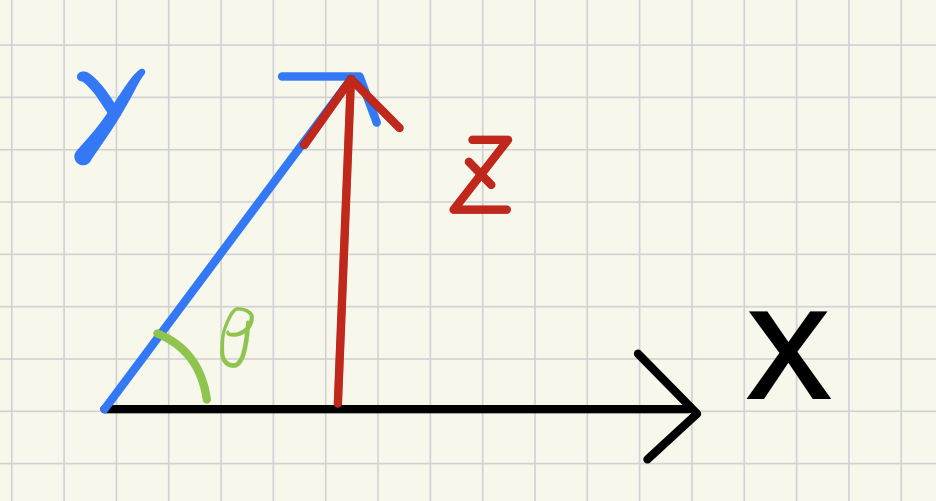
\includegraphics[height=5cm,width=12cm]{CSp.jpeg}
   \end{minipage}
\end{center}
Then all we do rest is just expanding $\abso{y}^2=\abso{z+\tilde{x}}^2$, where $\tilde{x}=y-z=\abso{y}(\cos \theta)\hat{x}$, which give the answer and is easy to compute since $z\cdot \tilde{x}=0$.\\

Now, with Cauchy-Schwarz Inequality, we can check the triangle inequality 
\begin{align*}
  \norm{x+y}^2&=\langle x+y,x+y\rangle \\
&=\langle x,x\rangle +\langle x,y\rangle +\langle y,x\rangle +\langle y,y\rangle \\
&= \langle x,x\rangle + \langle y,y\rangle +2\text{ Re }\langle x,y\rangle \\
&\leq \norm{x}^2 + \norm{y}^2 + 2\abso{\langle x,y\rangle }\\
&\leq \norm{x}^2 + \norm{y}^2 + 2\norm{x}\cdot \norm{y}=\Big(\norm{x}+\norm{y}\Big)^2
\end{align*}
\end{mdframed}
\textbf{(Euclidean Space Abstract Part)} 
\begin{mdframed}
  By a \textbf{concrete Euclidean Space}, we mean some space of $n$-tuple  $(x_1,\dots ,x_n)$ over $\R$, equipped with inner product  $\langle \cdot,\cdot\rangle_E$ defined by 
\begin{align*}
  \langle  (x_1,\dots,x_n)  ,(y_1,\dots ,y_n)\rangle_E= \sqrt{\sum_{k=1}^n (y_k-x_k)^2} 
\end{align*}
By an \textbf{Euclidean Space}, we simply mean a finite dimensional vector space $V$ over $\R$,  equipped with an inner product $\langle \cdot,\cdot\rangle $ such that there exists a concrete Euclidean space $E$ and an isomorphism  $\phi:V\to E$ such that 
\begin{align*}
\hspace{3cm}\langle x,y\rangle= \langle \phi (x),\phi (y)\rangle_E \hspace{1.5cm}(x,y \in V)
\end{align*}
Note that if you define $\langle \cdot,\cdot\rangle $ on the space of $n$-tuples $(x_1,\dots ,x_n)$ over $\R$ by 
\begin{align*}
  \langle  (x_1,\dots,x_n)  ,(y_1,\dots ,y_n)\rangle=2 \sqrt{\sum_{k=1}^n (y_k-x_k)^2} 
\end{align*}
Then, the space of $n$-tuple is clearly not a concrete Euclidean space, and clearly an Euclidean space. 

\end{mdframed}
\textbf{(SVD)}

\chapter{Beauty}
\section{$e^{iz}=\cos (z)+ i \sin (z)$}
\begin{mdframed}
Suppose that we define 
\begin{align*}
  \hspace{2cm}\exp(z)&\triangleq \sum_{n=0}^\infty \frac{z^n}{n!}\hspace{1.5cm}(z\inc)\\
  \hspace{2cm}\sin (z)&\triangleq \sum_{n=0}^\infty \frac{(-1)^n}{(2n+1)!}z^{2n+1}\hspace{1.5cm}(z\inc)\\
  \hspace{2cm}\cos (z)&\triangleq \sum_{n=0}^\infty \frac{(-1)^n}{(2n)!}z^{2n}\hspace{1.5cm}(z\inc)
\end{align*}
Some properties we are familiar with is now easily seen using basic technique we learned in Chapter 3. 
\begin{enumerate}[label=(\alph*)]
  \item $\exp(z),\sin(z),\cos(z)$ are well defined on $\C$ by \myref{Cauchy-Hadamard}{Cauchy-Hadamard}.  
  \item $\begin{cases}
    \exp(x)\\
    \sin(x)\\
    \cos(x)
  \end{cases}\inr$ provided $x\inr$. 
  \item $\begin{cases}
    \exp(0)=1 \\
    \sin(0)=0\\
    \cos (0)=1
  \end{cases}$
  \item $\exp(x)$ is strictly increasing on $\R\hspace{0.5cm}(\because \abso{y^n-x^n}\leq \abso{y^n}+\abso{x^n})$
  \item $\exp(x)\nearrow \infty$ as $x\to \infty\hspace{0.5cm}(x\inr)$ 
  \item $\exp(x)\cdot \exp(y)=\exp(x+y)\hspace{0.5cm}(x\inc)$ by \myref{Merten's Theorem of Cauchy Product}{Merten Cau}
  \item $\exp (x)\searrow 0$ as $x \to -\infty\hspace{0.5cm}(x\inr)$
  \item $\begin{cases}
\frac{d}{dz}\exp(z)=\exp(z)\\
  \frac{d}{dz}\sin (z)=\cos (z)\\
  \frac{d}{dz}\cos (z)=- \sin (z)
  \end{cases}(z\inc)$, using \myref{Term-by-Term Differentiation}{AfaS}. 
  \item $\exp (x)$ is convex on $\R\hspace{0.5cm}(\because (e^x)''=e^x>0)$  
  \item $\exp (nz)=\big(\exp (z) \big)^n\hspace{0.5cm}(z\inc,n\inz)$, by induction and \myref{Merten's Theorem of Cauchy Product}{Merten Cau}. 
\end{enumerate}
In particular, we have \textbf{Euler's Formula}. 
\end{mdframed}
\begin{theorem}
\textbf{(Euler's Formula)}  
\begin{align*}
\hspace{2cm}\exp(iz)=\cos (z) + i \sin (z)\hspace{1.5cm}(z\inc)
\end{align*}
\end{theorem}
\begin{proof}
Define 
\begin{align*}
I(n)\triangleq \begin{cases}
  1& \text{ if $n \equiv 0$ (mod $4$) }\\
  i& \text{ if $n \equiv 1$ (mod $4$) }\\
  -1& \text{ if $n \equiv 2$ (mod $4$) }\\
  -i& \text{ if $n \equiv 3$ (mod $4$) }
\end{cases}
\end{align*}
Compute 
\begin{align}
\label{expiz}
\exp(iz)&=\sum_{n=0}^\infty \frac{(iz)^n}{n!}\notag\\ 
&=\sum_{n=0}^{\infty} \frac{I(n)z^n}{n!}\\
&=\sum_{n=0}^{\infty} \frac{I(2n)}{(2n)!}z^{2n}+\frac{I(2n+1)}{(2n+1)!}z^{2n+1}\hspace{0.5cm}\big(\because \text{ this is a sub-sequence of \myref{(}{expiz})}\big)\notag\\
&= \sum_{n=0}^{\infty} \frac{(-1)^{n}}{(2n)!}z^{2n}+ i\cdot \frac{(-1)^n}{(2n+1)!}z^{2n+1} \notag
\end{align}
Now, we can conclude 
\begin{align*}
\cos (z)+i \sin (z)&= \sum_{n=0}^{\infty}\frac{(-1)^{n}}{(2n)!}z^{2n} + i \cdot \sum_{n=0}^{\infty} \frac{(-1)^{n}}{(2n+1)!}z^{2n+1}\\
&=\sum_{n=0}^{\infty}\frac{(-1)^{n}}{(2n)!}z^{2n} +  \sum_{n=0}^{\infty} i\cdot  \frac{(-1)^{n}}{(2n+1)!}z^{2n+1} \\
&=\sum_{n=0}^{\infty}\frac{(-1)^{n}}{(2n)!}z^{2n} +  i\cdot  \frac{(-1)^{n}}{(2n+1)!}z^{2n+1} =\exp (iz)
\end{align*}
\end{proof}


\section{$e^z$}
\begin{theorem}
\textbf{(First Characterization)} for all $x\inr$, the sequence $\set{(1+\frac{x}{n})^n}_{n\inn}$ has limit 
\begin{align*}
\lim_{n\to \infty} \Big(1+\frac{x}{n}\Big)^n = \sum_{k=0}^\infty \frac{x^k}{k!}
\end{align*}
\end{theorem}
\begin{proof}
The proof is trivial if $x=0$. First suppose  $x\inr^+$. Set 
\begin{align*}
t_n\triangleq \Big(1+\frac{x}{n}\Big)^n\text{ and }s_n\triangleq \sum_{k=0}^n \frac{x^k}{k!}
\end{align*}
We wish to show 
\begin{align*}
\vi{\limsup_{n\to\infty} t_n\leq \lim_{n\to \infty}s_n\leq \liminf_{n\to\infty} t_n}
\end{align*}
We first prove 
\begin{align*}
\blue{\limsup_{n\to\infty} t_n\leq \lim_{n\to \infty}s_n}
\end{align*}
Use Binomial Theorem to compute 
\begin{align*}
t_n=\Big(1+\frac{x}{n} \Big)^n&= \sum_{k=0}^n \binom{n}{k} \Big(\frac{x}{n} \Big)^k\\
&=\sum_{k=0}^n \frac{x^k}{k!} \cdot \frac{n(n-1)\cdots (n-k+1)}{n^k} \leq \sum_{k=0}^n \frac{x^k}{k!}=s_n \bdone
\end{align*}
We now prove 
\begin{align*}
\olive{\lim_{n\to \infty}s_n\leq \liminf_{n\to\infty} t_n}
\end{align*}
Fix $\epsilon $. Because $s_n\nearrow $, we know there exists  $m$ such that 
 \begin{align*}
s_m> \lim_{n\to \infty}s_n -\epsilon 
\end{align*}
Fix such $m$. Observe 
 \begin{align*}
\hspace{1.5cm}t_n=\sum _{k=0}^n \binom{n}{k}\Big(\frac{x}{n} \Big)^k\geq \sum_{k=0}^m \frac{x^k}{k!}\cdot \frac{n(n-1)\cdots (n-k+1)}{n^k}\hspace{1.5cm}(n\geq m)
\end{align*}
Clearly, there exists $N$ such that 
\begin{align*}
  \forall n>N, \abso{\Big( \sum_{k=0}^m \frac{x^k}{k!}\cdot \frac{n(n-1)\cdots (n-k+1)}{n^k}\Big) - s_m }\leq  s_m-(\lim_{n\to \infty}s_n-\epsilon )
\end{align*}
Then, we see for all $n>\max \set{N,m}$
\begin{align*}
  t_n\geq \sum_{k=0}^m \frac{x^k}{k!}\cdot \frac{n(n-1)\cdots (n-k+1)}{n^k} &\geq s_m - (s_m-\lim_{n\to \infty}s_n -\epsilon )\\
  &=\lim_{n\to \infty}s_n -\epsilon \odone \vdone
\end{align*}
For negative real, we only wish to show 
\begin{align*}
\vi{\sum_{n=0}^\infty \frac{(-x)^n}{n!}=\Big(\sum_{n=0}^\infty \frac{x^n}{n!} \Big)^{-1}}\text{ and }\blue{\lim_{n\to \infty}\Big(1-\frac{x}{n} \Big)^{n}=\Bigg(\lim_{n\to\infty    }\Big(1+\frac{x}{n} \Big)^{n} \Bigg)^{-1}}
\end{align*}
Because the convergence is absolute, we can use Merten's Theorem for Cauchy product (\myref{Theorem}{Merten Cau})to compute 
\begin{align*}
\Big( \sum_{n=0}^{\infty} \frac{(-x)^n}{n!}\Big)\cdot \Big( \sum_{n=0}^\infty \frac{x^n}{n!} \Big)&= \sum_{n=0}^\infty \Big(\sum_{k=0}^n \binom{n}{k}(-1)^{n-k} \Big) \frac{x^n}{n!}\\
&=\sum_{n=0}^\infty (1-1)^{n} \frac{x^n}{n!}=1 \vdone
\end{align*}
We first prove 
\begin{align*}
\olive{\lim_{n\to \infty}\Big(1-\frac{x^2}{n^2} \Big)^n=1}
\end{align*}
Computing term by term, it is clear that 
\begin{align*}
\limsup_{n\to\infty} \Big(1-\frac{x^2}{n^2} \Big)^n \leq 1
\end{align*}
Using Bernoulli's Inequality (\myref{Theorem}{Bernoulli's Inequality}), we see that for large enough $n$, we have 
\begin{align*}
  \Big(1-\frac{x^2}{n^2} \Big)^n\geq 1-\frac{x^2}{n} 
\end{align*}
This then implies 
\begin{align*}
\liminf_{n\to\infty} \Big(1-\frac{x^2}{n^2} \Big)^n \geq 1\odone
\end{align*}
Compute
\begin{align*}
\lim_{n\to \infty}\Big(1-\frac{x}{n} \Big)^{n} &= \lim_{n\to \infty}\Bigg(\frac{1-\frac{x^2}{n^2}}{1+\frac{x}{n}}\Bigg)^n \\
&=\frac{\lim_{n \to \infty} (1-\frac{x^2}{n^2})^n}{\lim_{n\to \infty}(1+\frac{x}{n})^n}=\frac{1}{\lim_{n\to \infty}(1+\frac{x}{n})^n}\bdone
\end{align*}





\end{proof}
\begin{mdframed}
\begin{align*}
\ln (x)\triangleq \int_1^x \frac{1}{t}dt
\end{align*}
By FTC (\myref{Theorem}{FTC1}), it is easy to see that 
 \begin{align*}
\hspace{1.5cm}\frac{d}{dx}\ln (x)=\frac{1}{x}\hspace{1.5cm}(x\inr^+)
\end{align*}
To see 
\begin{align*}
\ln (xy)=\ln (x)+ \ln (y)
\end{align*}
Fix $y\inr^+$ and set 
\begin{align*}
f(x)\triangleq \ln (x)\text{ and }g(x)\triangleq \ln(xy)
\end{align*}
Conclude $f'(x)=g'(x)$, and use FTC (\myref{Theorem}{FTC2}) to conclude $f-g$ is some fixed constant $k$. Now, see that 
\begin{align*}
g(1)=f(1)+k \implies k=\ln(y)
\end{align*}
Then, we have 
\begin{align*}
\ln(xy)=g(x)=f(x)+k=\ln (x)+ \ln (y)
\end{align*}
Using induction, it is now easy to see 
\begin{align*}
  \hspace{3cm}\ln (x^n)=n \ln (x)\hspace{2.5cm}(n\inz_0^+)
\end{align*}
\end{mdframed}
\begin{theorem}
\textbf{(Second Characterization)}
\end{theorem}
\section{$\sin$}
\section{Fundamental Theorem of Algebra}
\begin{theorem}
\textbf{(Fundamental Theorem of Algebra)}
\end{theorem}


\chapter{and the Beast}
\section{Weierstrass Function}
\section{Fabius Function}

\section{Cantor Set}
\section{Cantor-Lebesgue Function}
\section{Volterra's Function}
\section{Peano Space-filling Curve}



\end{document}
